%&preformat-disser
\RequirePackage[l2tabu,orthodox]{nag} % Раскомментировав, можно в логе получать рекомендации относительно правильного использования пакетов и предупреждения об устаревших и нерекомендуемых пакетах
% Формат А4, 14pt (ГОСТ Р 7.0.11-2011, 5.3.6)
\documentclass[a4paper,14pt,oneside,openany]{memoir}

%%%%%%%%%%%%%%%%%%%%%%%%%%%%%%%%%%%%%%%%%%%%%%%%%%%%%%%%%%%%%%%%%%%%%%%%%%%%%%%%
%%%% Файл упрощённых настроек шаблона, общих для диссертации и автореферата %%%%
%%%%%%%%%%%%%%%%%%%%%%%%%%%%%%%%%%%%%%%%%%%%%%%%%%%%%%%%%%%%%%%%%%%%%%%%%%%%%%%%

%%% Режим черновика %%%
\makeatletter
\@ifundefined{c@draft}{
  \newcounter{draft}
  \setcounter{draft}{0}  % 0 --- чистовик (максимальное соблюдение ГОСТ)
                         % 1 --- черновик (отклонения от ГОСТ, но быстрая
                         %       сборка итоговых PDF)
}{}
\makeatother

%%% Использование в pdflatex шрифтов не по-умолчанию %%%
\makeatletter
\@ifundefined{c@usealtfont}{
  \newcounter{usealtfont}
  \setcounter{usealtfont}{1}    % 0 --- шрифты на базе Computer Modern
                                % 1 --- использовать пакет pscyr, при его
                                %       наличии
                                % 2 --- использовать пакет XCharter, при наличии
                                %       подходящей версии
}{}
\makeatother

%%% Использование в xelatex и lualatex семейств шрифтов %%%
\makeatletter
\@ifundefined{c@fontfamily}{
  \newcounter{fontfamily}
  \setcounter{fontfamily}{1}  % 0 --- CMU семейство. Используется как fallback;
                              % 1 --- Шрифты от MS (Times New Roman и компания)
                              % 2 --- Семейство Liberation
}{}
\makeatother

%%% Библиография %%%
\makeatletter
\@ifundefined{c@bibliosel}{
  \newcounter{bibliosel}
  \setcounter{bibliosel}{1}   % 0 --- встроенная реализация с загрузкой файла
                              %       через движок bibtex8;
                              % 1 --- реализация пакетом biblatex через движок
                              %       biber
}{}
\makeatother

%%% Предкомпиляция tikz рисунков для ускорения работы %%%
\makeatletter
\@ifundefined{c@imgprecompile}{
  \newcounter{imgprecompile}
  \setcounter{imgprecompile}{0}   % 0 --- без предкомпиляции;
                                  % 1 --- пользоваться предварительно
                                  %       скомпилированными pdf вместо генерации
                                  %       заново из tikz
}{}
\makeatother
            % общие настройки шаблона
%%% Проверка используемого TeX-движка %%%
\RequirePackage{ifxetex, ifluatex}
\newif\ifxetexorluatex   % определяем новый условный оператор (http://tex.stackexchange.com/a/47579)
\ifxetex
    \xetexorluatextrue
\else
    \ifluatex
        \xetexorluatextrue
    \else
        \xetexorluatexfalse
    \fi
\fi

\newif\ifsynopsis           % Условие, проверяющее, что документ --- автореферат

\RequirePackage{etoolbox}[2015/08/02]               % Для продвинутой проверки разных условий
\providebool{presentation}

%%% Поля и разметка страницы %%%
\usepackage{pdflscape}                              % Для включения альбомных страниц
\usepackage{geometry}                               % Для последующего задания полей

%%% Математические пакеты %%%
\usepackage{amsthm,amsmath,amscd}   % Математические дополнения от AMS
\usepackage{amsfonts,amssymb}       % Математические дополнения от AMS
\usepackage{mathtools}              % Добавляет окружение multlined

%%%% Установки для размера шрифта 14 pt %%%%
%% Формирование переменных и констант для сравнения (один раз для всех подключаемых файлов)%%
%% должно располагаться до вызова пакета fontspec или polyglossia, потому что они сбивают его работу
\newlength{\curtextsize}
\newlength{\bigtextsize}
\setlength{\bigtextsize}{13.9pt}

\makeatletter
%\show\f@size                                       % неплохо для отслеживания, но вызывает стопорение процесса, если документ компилируется без команды  -interaction=nonstopmode
\setlength{\curtextsize}{\f@size pt}
\makeatother

%%% Кодировки и шрифты %%%
\ifxetexorluatex
    \usepackage{polyglossia}[2014/05/21]            % Поддержка многоязычности (fontspec подгружается автоматически)
\else
   %%% Решение проблемы копирования текста в буфер кракозябрами
    \ifnumequal{\value{usealtfont}}{0}{}{
        \input glyphtounicode.tex
        \input glyphtounicode-cmr.tex %from pdfx package
        \pdfgentounicode=1
    }
    \usepackage{cmap}                               % Улучшенный поиск русских слов в полученном pdf-файле
    \ifnumequal{\value{usealtfont}}{2}{}{
        \defaulthyphenchar=127                      % Если стоит до fontenc, то переносы не впишутся в выделяемый текст при копировании его в буфер обмена
    }
    \usepackage{textcomp}
    \usepackage[T1,T2A]{fontenc}                    % Поддержка русских букв
    \ifnumequal{\value{usealtfont}}{1}{% Используется pscyr, при наличии
        \IfFileExists{pscyr.sty}{\usepackage{pscyr}}{}  % Подключение pscyr
    }{}
    \usepackage[utf8]{inputenc}[2014/04/30]         % Кодировка utf8
    \usepackage[english, russian]{babel}[2014/03/24]% Языки: русский, английский
    \ifnumequal{\value{usealtfont}}{2}{
        % http://dxdy.ru/post1238763.html#p1238763
        \usepackage[scaled=0.960]{XCharter}[2017/12/19] % Подключение русифицированных шрифтов XCharter
        \usepackage[charter, vvarbb, scaled=1.048]{newtxmath}[2017/12/14]
        \setDisplayskipStretch{-0.078}
    }{}
\fi

%%% Оформление абзацев %%%
\usepackage{indentfirst}                            % Красная строка

%%% Цвета %%%
\ifpresentation
\else
    \usepackage[dvipsnames, table, hyperref]{xcolor} % Совместимо с tikz
\fi

%%% Таблицы %%%
\usepackage{longtable,ltcaption}                    % Длинные таблицы
\usepackage{multirow,makecell}                      % Улучшенное форматирование таблиц

%%% Общее форматирование
\usepackage{soulutf8}                               % Поддержка переносоустойчивых подчёркиваний и зачёркиваний
\usepackage{icomma}                                 % Запятая в десятичных дробях

%%% Оптимизация расстановки переносов и длины последней строки абзаца
\IfFileExists{impnattypo.sty}{% проверка установленности пакета impnattypo
    \ifluatex
        \ifnumequal{\value{draft}}{1}{% Черновик
            \usepackage[hyphenation, lastparline, nosingleletter, homeoarchy,
            rivers, draft]{impnattypo}
        }{% Чистовик
            \usepackage[hyphenation, lastparline, nosingleletter]{impnattypo}
        }
    \else
        \usepackage[hyphenation, lastparline]{impnattypo}
    \fi
}{}

%%% Гиперссылки %%%
\usepackage{hyperref}[2012/11/06]

%%% Изображения %%%
\usepackage{graphicx}[2014/04/25]                   % Подключаем пакет работы с графикой

%%% Счётчики %%%
\usepackage[figure,table]{totalcount}               % Счётчик рисунков и таблиц
\usepackage{totcount}                               % Пакет создания счётчиков на основе последнего номера подсчитываемого элемента (может требовать дважды компилировать документ)
\usepackage{totpages}                               % Счётчик страниц, совместимый с hyperref (ссылается на номер последней страницы). Желательно ставить последним пакетом в преамбуле

%%% Продвинутое управление групповыми ссылками (пока только формулами) %%%
\ifpresentation
\else
    \ifxetexorluatex
        \usepackage{cleveref}                           % cleveref корректно считывает язык из настроек polyglossia
    \else
        \usepackage[russian]{cleveref}                  % cleveref имеет сложности со считыванием языка из babel. Такое решение русификации вывода выбрано вместо определения в documentclass из опасности что-то лишнее передать во все остальные пакеты, включая библиографию.
    \fi
    \creflabelformat{equation}{#2#1#3}                  % Формат по умолчанию ставил круглые скобки вокруг каждого номера ссылки, теперь просто номера ссылок без какого-либо дополнительного оформления
    \crefrangelabelformat{equation}{#3#1#4\cyrdash#5#2#6}   % Интервалы в русском языке принято делать через тире, если иное не оговорено

    % решение проблемы с "и" в \labelcref
    % https://tex.stackexchange.com/a/455124/104425
    \ifxetexorluatex
        \DeclareTextSymbol{\cyri}\UnicodeEncodingName{"0438} % и
    \fi

    % Добавление возможности использования пробелов в \labelcref
    % https://tex.stackexchange.com/a/340502/104425
    \usepackage{kvsetkeys}
    \makeatletter
    \let\org@@cref\@cref
    \renewcommand*{\@cref}[2]{%
        \edef\process@me{%
            \noexpand\org@@cref{#1}{\zap@space#2 \@empty}%
        }\process@me
    }
    \makeatother
\fi

\ifnumequal{\value{draft}}{1}{% Черновик
    \usepackage[firstpage]{draftwatermark}
    \SetWatermarkText{DRAFT}
    \SetWatermarkFontSize{14pt}
    \SetWatermarkScale{15}
    \SetWatermarkAngle{45}
}{}

%%% Исправление положения якорей подписей (под)рисунков %%%
% Без hypcap и патча, при клике по ссылке на подрисунок, просмотрщик pdf прыгает "к подписи" а не "к рисунку".
% Подробнее: https://github.com/AndreyAkinshin/Russian-Phd-LaTeX-Dissertation-Template/issues/238
% (!) Даже с патчем, если мешать в одной фиге разные типы подфиг (subbottom и subcaption) - ссылки всё равно будут работать неправильно  (см. https://www.overleaf.com/read/czmbmmtnqrrg ).
\ifpresentation
\else
    \usepackage[all]{hypcap}

    \makeatletter
    \ltx@ifclasslater{memoir}{2018/12/13}{
        % Предполагается, что в следующей версии класс будет исправлен
        \typeout{Assuming this version of memoir is free from the jumping-to-caption bug.}
    }{
        \RequirePackage{xpatch}

        \newcommand\mem@step@subcounter{\refstepcounter{sub\@captype}\@contkeep}

        \xpatchcmd{\@memsubbody}%
        {\refstepcounter{sub\@captype}\@contkeep}% search pattern
        {}% replacement
        {\typeout{@memsubbody is patched}}%
        {\typeout{@memsubbody is NOT patched}}%

        \xpatchcmd{\@memcontsubbody}%
        {\refstepcounter{sub\@captype}\@contkeep}% pattern
        {}% replacement
        {\typeout{@memcontsubbody is patched}}%
        {\typeout{@memcontsubbody is NOT patched}}%

        \xpatchcmd{\@memsubfloat}%
        {\vbox\bgroup}% search pattern
        {\vbox\bgroup\mem@step@subcounter}% replacement
        {\typeout{@memsubfloat patch is ok}}%
        {\typeout{@memsubfloat patch is NOT ok}}%

        \xpatchcmd{\subcaption}%
        {\refstepcounter{sub\@captype}}% search pattern
        {\H@refstepcounter{sub\@captype}}% replacement
        {\typeout{subcaption second patch is ok}}%
        {\typeout{subcaption second patch is NOT ok}}%
    }
    \makeatother
\fi

%%% Цитата, не приводимая в автореферате:
% возможно, актуальна только для biblatex
%\newcommand{\citeinsynopsis}[1]{\ifsynopsis\else ~\cite{#1} \fi}

%% Векторная графика

\usepackage{tikz}                   % Продвинутый пакет векторной графики
\usetikzlibrary{chains}             % Для примера tikz рисунка
\usetikzlibrary{shapes.geometric}   % Для примера tikz рисунка
\usetikzlibrary{shapes.symbols}     % Для примера tikz рисунка
\usetikzlibrary{arrows}             % Для примера tikz рисунка

% если текущий процесс запущен библиотекой tikz-external, то прекомпиляция должна быть включена
\ifdefined\tikzexternalrealjob
    \setcounter{imgprecompile}{1}
\fi

\ifnumequal{\value{imgprecompile}}{1}{% Только если у нас включена предкомпиляция
    \usetikzlibrary{external}   % подключение возможности предкомпиляции
    \tikzexternalize[prefix=images/cache/] % activate! % здесь можно указать отдельную папку для скомпилированных файлов
    \ifxetex
        \tikzset{external/up to date check={diff}}
    \fi
}{}
         % Пакеты общие для диссертации и автореферата
\synopsisfalse                      % Этот документ --- не автореферат
%%% Прикладные пакеты %%%
%\usepackage{calc}               % Пакет для расчётов параметров, например длины

%%% Для добавления Стр. над номерами страниц в оглавлении
%%% http://tex.stackexchange.com/a/306950
\usepackage{afterpage}

%%% Списки %%%
\usepackage{enumitem}

\usepackage{tikz}                   % Продвинутый пакет векторной графики
\usetikzlibrary{chains}             % Для примера tikz рисунка
\usetikzlibrary{shapes.geometric}   % Для примера tikz рисунка
\usetikzlibrary{shapes.symbols}     % Для примера tikz рисунка
\usetikzlibrary{arrows}             % Для примера tikz рисунка
\ifnumequal{\value{imgprecompile}}{1}{% Только если у нас включена предкомпиляция
    \usetikzlibrary{external}   % подключение возможности предкомпиляции
    \tikzexternalize[prefix=Dissertation/images/] % activate! % здесь можно указать отдельную папку для скомпилированных файлов
    \ifxetex
        \tikzset{external/up to date check={diff}}
    \fi
}{}
    % Пакеты для диссертации
\usepackage{tabu, tabulary}  %таблицы с автоматически подбирающейся шириной столбцов
\usepackage{fr-longtable}    %ради \endlasthead

% Листинги с исходным кодом программ
\usepackage{fancyvrb}
\usepackage{listings}
\lccode`\~=0\relax %Без этого хака из-за особенностей пакета listings перестают работать конструкции с \MakeLowercase и т. п. в (xe|lua)latex

% Русская традиция начертания греческих букв
\usepackage{upgreek} % прямые греческие ради русской традиции

%%% Микротипографика
%\ifnumequal{\value{draft}}{0}{% Только если у нас режим чистовика
%    \usepackage[final, babel, shrink=45]{microtype}[2016/05/14] % улучшает представление букв и слов в строках, может помочь при наличии отдельно висящих слов
%}{}

% Отметка о версии черновика на каждой странице
% Чтобы работало надо в своей локальной копии по инструкции
% https://www.ctan.org/pkg/gitinfo2 создать небходимые файлы в папке
% ./git/hooks
% If you’re familiar with tweaking git, you can probably work it out for
% yourself. If not, I suggest you follow these steps:
% 1. First, you need a git repository and working tree. For this example,
% let’s suppose that the root of the working tree is in ~/compsci
% 2. Copy the file post-xxx-sample.txt (which is in the same folder of
% your TEX distribution as this pdf) into the git hooks directory in your
% working copy. In our example case, you should end up with a file called
% ~/compsci/.git/hooks/post-checkout
% 3. If you’re using a unix-like system, don’t forget to make the file executable.
% Just how you do this is outside the scope of this manual, but one
% possible way is with commands such as this:
% chmod g+x post-checkout.
% 4. Test your setup with “git checkout master” (or another suitable branch
% name). This should generate copies of gitHeadInfo.gin in the directories
% you intended.
% 5. Now make two more copies of this file in the same directory (hooks),
% calling them post-commit and post-merge, and you’re done. As before,
% users of unix-like systems should ensure these files are marked as
% executable.
\ifnumequal{\value{draft}}{1}{% Черновик
   \IfFileExists{.git/gitHeadInfo.gin}{
      \usepackage[mark,pcount]{gitinfo2}
      \renewcommand{\gitMark}{rev.\gitAbbrevHash\quad\gitCommitterEmail\quad\gitAuthorIsoDate}
      \renewcommand{\gitMarkFormat}{\rmfamily\color{Gray}\small\bfseries}
   }{}
}{}   % Пакеты для специфических пользовательских задач

%%%%%%%%%%%%%%%%%%%%%%%%%%%%%%%%%%%%%%%%%%%%%%%%%%%%%%
%%%% Файл упрощённых настроек шаблона диссертации %%%%
%%%%%%%%%%%%%%%%%%%%%%%%%%%%%%%%%%%%%%%%%%%%%%%%%%%%%%

%%% Инициализирование переменных, не трогать!  %%%
\newcounter{intvl}
\newcounter{otstup}
\newcounter{contnumeq}
\newcounter{contnumfig}
\newcounter{contnumtab}
\newcounter{pgnum}
\newcounter{chapstyle}
\newcounter{headingdelim}
\newcounter{headingalign}
\newcounter{headingsize}
\newcounter{tabcap}
\newcounter{tablaba}
\newcounter{tabtita}
%%%%%%%%%%%%%%%%%%%%%%%%%%%%%%%%%%%%%%%%%%%%%%%%%%

%%% Область упрощённого управления оформлением %%%

%% Интервал между заголовками и между заголовком и текстом
% Заголовки отделяют от текста сверху и снизу тремя интервалами (ГОСТ Р 7.0.11-2011, 5.3.5)
\setcounter{intvl}{3}               % Коэффициент кратности к размеру шрифта

%% Отступы у заголовков в тексте
\setcounter{otstup}{0}              % 0 --- без отступа; 1 --- абзацный отступ

%% Нумерация формул, таблиц и рисунков
\setcounter{contnumeq}{0}           % Нумерация формул: 0 --- пораздельно (во введении подряд, без номера раздела); 1 --- сквозная нумерация по всей диссертации
\setcounter{contnumfig}{0}          % Нумерация рисунков: 0 --- пораздельно (во введении подряд, без номера раздела); 1 --- сквозная нумерация по всей диссертации
\setcounter{contnumtab}{1}          % Нумерация таблиц: 0 --- пораздельно (во введении подряд, без номера раздела); 1 --- сквозная нумерация по всей диссертации

%% Оглавление
\setcounter{pgnum}{1}               % 0 --- номера страниц никак не обозначены; 1 --- Стр. над номерами страниц (дважды компилировать после изменения)
\settocdepth{subsection}            % до какого уровня подразделов выносить в оглавление
\setsecnumdepth{subsection}         % до какого уровня нумеровать подразделы


%% Текст и форматирование заголовков
\setcounter{chapstyle}{1}           % 0 --- разделы только под номером; 1 --- разделы с названием "Глава" перед номером
\setcounter{headingdelim}{1}        % 0 --- номер отделен пропуском в 1em или \quad; 1 --- номера разделов и приложений отделены точкой с пробелом, подразделы пропуском без точки; 2 --- номера разделов, подразделов и приложений отделены точкой с пробелом.

%% Выравнивание заголовков в тексте
\setcounter{headingalign}{0}        % 0 --- по центру; 1 --- по левому краю

%% Размеры заголовков в тексте
\setcounter{headingsize}{0}         % 0 --- по ГОСТ, все всегда 14 пт; 1 --- пропорционально изменяющийся размер в зависимости от базового шрифта

%% Подпись таблиц
\setcounter{tabcap}{0}              % 0 --- по ГОСТ, номер таблицы и название разделены тире, выровнены по левому краю, при необходимости на нескольких строках; 1 --- подпись таблицы не по ГОСТ, на двух и более строках, дальнейшие настройки:
%Выравнивание первой строки, с подписью и номером
\setcounter{tablaba}{2}             % 0 --- по левому краю; 1 --- по центру; 2 --- по правому краю
%Выравнивание строк с самим названием таблицы
\setcounter{tabtita}{1}             % 0 --- по левому краю; 1 --- по центру; 2 --- по правому краю
%Разделитель записи «Таблица #» и названия таблицы
\newcommand{\tablabelsep}{ }

%% Подпись рисунков
%Разделитель записи «Рисунок #» и названия рисунка
\newcommand{\figlabelsep}{~\cyrdash\ } % (ГОСТ 2.105, 4.3.1) % "--- здесь не работает

%%% Цвета гиперссылок %%%
% Latex color definitions: http://latexcolor.com/
\definecolor{linkcolor}{rgb}{0.9,0,0}
\definecolor{citecolor}{rgb}{0,0.6,0}
\definecolor{urlcolor}{rgb}{0,0,1}
%\definecolor{linkcolor}{rgb}{0,0,0} %black
%\definecolor{citecolor}{rgb}{0,0,0} %black
%\definecolor{urlcolor}{rgb}{0,0,0} %black
      % Упрощённые настройки шаблона

% Новые переменные, которые могут использоваться во всём проекте
% ГОСТ 7.0.11-2011
% 9.2 Оформление текста автореферата диссертации
% 9.2.1 Общая характеристика работы включает в себя следующие основные структурные
% элементы:
% актуальность темы исследования;
\newcommand{\actualityTXT}{Актуальность темы.}
% степень ее разработанности;
\newcommand{\progressTXT}{Степень разработанности темы.}
% цели и задачи;
\newcommand{\aimTXT}{Цель работы}
\newcommand{\tasksTXT}{задачи}
% научную новизну;
\newcommand{\noveltyTXT}{Научная новизна}
% теоретическую и практическую значимость работы;
%\newcommand{\influenceTXT}{Теоретическая и практическая значимость}
% или чаще используют просто
\newcommand{\influenceTXT}{Практическая значимость}
% методологию и методы исследования;
\newcommand{\methodsTXT}{Методология и методы исследования.}
% положения, выносимые на защиту;
\newcommand{\defpositionsTXT}{Основные положения, выносимые на~защиту}
% степень достоверности и апробацию результатов.
\newcommand{\reliabilityTXT}{Достоверность результатов}
\newcommand{\probationTXT}{Апробация результатов}

\newcommand{\contributionTXT}{Личный вклад}
\newcommand{\publicationsTXT}{Публикации}


%%% Заголовки библиографии:

% для автореферата:
\newcommand{\bibtitleauthor}{Публикации автора по теме диссертации}

% для стиля библиографии `\insertbiblioauthorgrouped`
\newcommand{\bibtitleauthorvak}{В изданиях из списка ВАК РФ}
\newcommand{\bibtitleauthorscopus}{В изданиях, входящих в международную базу цитирования Scopus}
\newcommand{\bibtitleauthorwos}{В изданиях, входящих в международную базу цитирования Web of Science}
\newcommand{\bibtitleauthorother}{В прочих изданиях}
\newcommand{\bibtitleauthorconf}{В сборниках трудов конференций}

% для стиля библиографии `\insertbiblioauthorimportant`:
\newcommand{\bibtitleauthorimportant}{Наиболее значимые \protect\MakeLowercase\bibtitleauthor}

% для списка литературы в диссертации и списка чужих работ в автореферате:
\newcommand{\bibtitlefull}{Список литературы} % (ГОСТ Р 7.0.11-2011, 4)
         % Новые переменные, для всего проекта

%%% Основные сведения %%%
\newcommand{\thesisAuthorLastName}{\todo{Фамилия}}
\newcommand{\thesisAuthorOtherNames}{\todo{Имя Отчество}}
\newcommand{\thesisAuthorInitials}{\todo{И.\,О.}}
\newcommand{\thesisAuthor}             % Диссертация, ФИО автора
{%
    \texorpdfstring{% \texorpdfstring takes two arguments and uses the first for (La)TeX and the second for pdf
        \thesisAuthorLastName~\thesisAuthorOtherNames% так будет отображаться на титульном листе или в тексте, где будет использоваться переменная
    }{%
        \thesisAuthorLastName, \thesisAuthorOtherNames% эта запись для свойств pdf-файла. В таком виде, если pdf будет обработан программами для сбора библиографических сведений, будет правильно представлена фамилия.
    }
}
\newcommand{\thesisAuthorShort}        % Диссертация, ФИО автора инициалами
{\thesisAuthorInitials~\thesisAuthorLastName}
%\newcommand{\thesisUdk}                % Диссертация, УДК
%{\todo{xxx.xxx}}
\newcommand{\thesisTitle}              % Диссертация, название
{\todo{Название диссертационной работы}}
\newcommand{\thesisSpecialtyNumber}    % Диссертация, специальность, номер
{01.03.02}
\newcommand{\thesisSpecialtyTitle}     % Диссертация, специальность, название
{\todo{Название специальности}}
\newcommand{\thesisDegree}             % Диссертация, ученая степень
{\todo{кандидата физико-математических наук}}
\newcommand{\thesisDegreeShort}        % Диссертация, ученая степень, краткая запись
{\todo{канд. физ.-мат. наук}}
\newcommand{\thesisCity}               % Диссертация, город написания диссертации
{\todo{Город}}
\newcommand{\thesisYear}               % Диссертация, год написания диссертации
{\todo{20XX}}
\newcommand{\thesisOrganization}       % Диссертация, организация
{\todo{Название учреждения, в~котором выполнялась данная диссертационная работа}}
\newcommand{\thesisOrganizationShort}  % Диссертация, краткое название организации для доклада
{\todo{НазУчДисРаб}}

\newcommand{\thesisInOrganization}     % Диссертация, организация в предложном падеже: Работа выполнена в ...
{\todo{учреждении, в~котором выполнялась данная диссертационная работа}}

\newcommand{\supervisorFio}            % Научный руководитель, ФИО
{\todo{Фамилия Имя Отчество}}
\newcommand{\supervisorRegalia}        % Научный руководитель, регалии
{\todo{уч. степень, уч. звание}}
\newcommand{\supervisorFioShort}       % Научный руководитель, ФИО
{\todo{И.\,О.~Фамилия}}
\newcommand{\supervisorRegaliaShort}   % Научный руководитель, регалии
{\todo{уч.~ст.,~уч.~зв.}}


\newcommand{\opponentOneFio}           % Оппонент 1, ФИО
{\todo{Фамилия Имя Отчество}}
\newcommand{\opponentOneRegalia}       % Оппонент 1, регалии
{\todo{доктор физико-математических наук, профессор}}
\newcommand{\opponentOneJobPlace}      % Оппонент 1, место работы
{\todo{Не очень длинное название для места работы}}
\newcommand{\opponentOneJobPost}       % Оппонент 1, должность
{\todo{старший научный сотрудник}}

\newcommand{\opponentTwoFio}           % Оппонент 2, ФИО
{\todo{Фамилия Имя Отчество}}
\newcommand{\opponentTwoRegalia}       % Оппонент 2, регалии
{\todo{кандидат физико-математических наук}}
\newcommand{\opponentTwoJobPlace}      % Оппонент 2, место работы
{\todo{Основное место работы c длинным длинным длинным длинным названием}}
\newcommand{\opponentTwoJobPost}       % Оппонент 2, должность
{\todo{старший научный сотрудник}}

\newcommand{\leadingOrganizationTitle} % Ведущая организация, дополнительные строки
{\todo{Федеральное государственное бюджетное образовательное учреждение высшего профессионального образования с~длинным длинным длинным длинным названием}}

\newcommand{\defenseDate}              % Защита, дата
{\todo{DD mmmmmmmm YYYY~г.~в~XX часов}}
\newcommand{\defenseCouncilNumber}     % Защита, номер диссертационного совета
{\todo{Д\,123.456.78}}
\newcommand{\defenseCouncilTitle}      % Защита, учреждение диссертационного совета
{\todo{Название учреждения}}
\newcommand{\defenseCouncilAddress}    % Защита, адрес учреждение диссертационного совета
{\todo{Адрес}}
\newcommand{\defenseCouncilPhone}      % Телефон для справок
{\todo{+7~(0000)~00-00-00}}

\newcommand{\defenseSecretaryFio}      % Секретарь диссертационного совета, ФИО
{\todo{Фамилия Имя Отчество}}
\newcommand{\defenseSecretaryRegalia}  % Секретарь диссертационного совета, регалии
{\todo{д-р~физ.-мат. наук}}            % Для сокращений есть ГОСТы, например: ГОСТ Р 7.0.12-2011 + http://base.garant.ru/179724/#block_30000

\newcommand{\synopsisLibrary}          % Автореферат, название библиотеки
{\todo{Название библиотеки}}
\newcommand{\synopsisDate}             % Автореферат, дата рассылки
{\todo{DD mmmmmmmm YYYY года}}

% To avoid conflict with beamer class use \providecommand
\providecommand{\keywords}%            % Ключевые слова для метаданных PDF диссертации и автореферата
{}
             % Основные сведения
%%% Кодировки и шрифты %%%
\ifxetexorluatex
    % Язык по-умолчанию русский с поддержкой приятных команд пакета babel
    \ifnewpoly
        \setmainlanguage[babelshorthands=true,indentfirst=true]{russian}
    \else
        \setmainlanguage[babelshorthands=true]{russian}
    \fi
    \setotherlanguage{english}                         % Дополнительный язык = английский (в американской вариации по-умолчанию)

    % Проверка существования шрифтов. Недоступна в pdflatex
    \ifnumequal{\value{fontfamily}}{1}{
        \IfFontExistsTF{Times New Roman}{}{\setcounter{fontfamily}{0}}
    }{}
    \ifnumequal{\value{fontfamily}}{2}{
        \IfFontExistsTF{LiberationSerif}{}{\setcounter{fontfamily}{0}}
    }{}

    \ifnumequal{\value{fontfamily}}{0}{                    % Семейство шрифтов CMU. Используется как fallback
        \setmonofont{CMU Typewriter Text}                  % моноширинный шрифт
        \newfontfamily\cyrillicfonttt{CMU Typewriter Text} % моноширинный шрифт для кириллицы
        \defaultfontfeatures{Ligatures=TeX}                % стандартные лигатуры TeX, замены нескольких дефисов на тире и т. п. Настройки моноширинного шрифта должны идти до этой строки, чтобы при врезках кода программ в коде не применялись лигатуры и замены дефисов
        \setmainfont{CMU Serif}                            % Шрифт с засечками
        \newfontfamily\cyrillicfont{CMU Serif}             % Шрифт с засечками для кириллицы
        \setsansfont{CMU Sans Serif}                       % Шрифт без засечек
        \newfontfamily\cyrillicfontsf{CMU Sans Serif}      % Шрифт без засечек для кириллицы
    }

    \ifnumequal{\value{fontfamily}}{1}{                    % Семейство MS шрифтов
        \setmonofont{Courier New}                          % моноширинный шрифт
        \newfontfamily\cyrillicfonttt{Courier New}         % моноширинный шрифт для кириллицы
        \defaultfontfeatures{Ligatures=TeX}                % стандартные лигатуры TeX, замены нескольких дефисов на тире и т. п. Настройки моноширинного шрифта должны идти до этой строки, чтобы при врезках кода программ в коде не применялись лигатуры и замены дефисов
        \setmainfont{Times New Roman}                      % Шрифт с засечками
        \newfontfamily\cyrillicfont{Times New Roman}       % Шрифт с засечками для кириллицы
        \setsansfont{Arial}                                % Шрифт без засечек
        \newfontfamily\cyrillicfontsf{Arial}               % Шрифт без засечек для кириллицы
    }

    \ifnumequal{\value{fontfamily}}{2}{                    % Семейство шрифтов Liberation (https://pagure.io/liberation-fonts)
        \setmonofont{LiberationMono}[Scale=0.87] % моноширинный шрифт
        \newfontfamily\cyrillicfonttt{LiberationMono}[     % моноширинный шрифт для кириллицы
            Scale=0.87]
        \defaultfontfeatures{Ligatures=TeX}                % стандартные лигатуры TeX, замены нескольких дефисов на тире и т. п. Настройки моноширинного шрифта должны идти до этой строки, чтобы при врезках кода программ в коде не применялись лигатуры и замены дефисов
        \setmainfont{LiberationSerif}                      % Шрифт с засечками
        \newfontfamily\cyrillicfont{LiberationSerif}       % Шрифт с засечками для кириллицы
        \setsansfont{LiberationSans}                       % Шрифт без засечек
        \newfontfamily\cyrillicfontsf{LiberationSans}      % Шрифт без засечек для кириллицы
    }

\else
    \ifnumequal{\value{usealtfont}}{1}{% Используется pscyr, при наличии
        \IfFileExists{pscyr.sty}{\renewcommand{\rmdefault}{ftm}}{}
    }{}
\fi
            % Определение шрифтов (частичное)
%%% Шаблон %%%
\DeclareRobustCommand{\fixme}{\textcolor{red}}  % решаем проблему превращения
                                % названия цвета в результате \MakeUppercase,
                                % http://tex.stackexchange.com/a/187930,
                                % \DeclareRobustCommand protects \fixme
                                % from expanding inside \MakeUppercase
\AtBeginDocument{%
    \setlength{\parindent}{2.5em}                   % Абзацный отступ. Должен быть одинаковым по всему тексту и равен пяти знакам (ГОСТ Р 7.0.11-2011, 5.3.7).
}

%%% Таблицы %%%
\DeclareCaptionLabelSeparator{tabsep}{\tablabelsep} % нумерация таблиц
\DeclareCaptionFormat{split}{\splitformatlabel#1\par\splitformattext#3}

\captionsetup[table]{
        format=\tabformat,                % формат подписи (plain|hang)
        font=normal,                      % нормальные размер, цвет, стиль шрифта
        skip=.0pt,                        % отбивка под подписью
        parskip=.0pt,                     % отбивка между параграфами подписи
        position=above,                   % положение подписи
        justification=\tabjust,           % центровка
        indent=\tabindent,                % смещение строк после первой
        labelsep=tabsep,                  % разделитель
        singlelinecheck=\tabsinglecenter, % не выравнивать по центру, если умещается в одну строку
}

%%% Рисунки %%%
\DeclareCaptionLabelSeparator{figsep}{\figlabelsep} % нумерация рисунков

\captionsetup[figure]{
        format=plain,                     % формат подписи (plain|hang)
        font=normal,                      % нормальные размер, цвет, стиль шрифта
        skip=.0pt,                        % отбивка под подписью
        parskip=.0pt,                     % отбивка между параграфами подписи
        position=below,                   % положение подписи
        singlelinecheck=true,             % выравнивание по центру, если умещается в одну строку
        justification=centerlast,         % центровка
        labelsep=figsep,                  % разделитель
}

%%% Подписи подрисунков %%%
\DeclareCaptionSubType{figure}
\renewcommand\thesubfigure{\asbuk{subfigure}} % нумерация подрисунков
\ifsynopsis
\DeclareCaptionFont{norm}{\fontsize{10pt}{11pt}\selectfont}
\newcommand{\subfigureskip}{2.pt}
\else
\DeclareCaptionFont{norm}{\fontsize{14pt}{16pt}\selectfont}
\newcommand{\subfigureskip}{0.pt}
\fi

\captionsetup[subfloat]{
        labelfont=norm,                 % нормальный размер подписей подрисунков
        textfont=norm,                  % нормальный размер подписей подрисунков
        labelsep=space,                 % разделитель
        labelformat=brace,              % одна скобка справа от номера
        justification=centering,        % центровка
        singlelinecheck=true,           % выравнивание по центру, если умещается в одну строку
        skip=\subfigureskip,            % отбивка над подписью
        parskip=.0pt,                   % отбивка между параграфами подписи
        position=below,                 % положение подписи
}

%%% Настройки гиперссылок %%%
\ifluatex
    \hypersetup{
        unicode,                % Unicode encoded PDF strings
    }
\fi

\hypersetup{
    linktocpage=true,           % ссылки с номера страницы в оглавлении, списке таблиц и списке рисунков
%    linktoc=all,                % both the section and page part are links
%    pdfpagelabels=false,        % set PDF page labels (true|false)
    plainpages=false,           % Forces page anchors to be named by the Arabic form  of the page number, rather than the formatted form
    colorlinks,                 % ссылки отображаются раскрашенным текстом, а не раскрашенным прямоугольником, вокруг текста
    linkcolor={linkcolor},      % цвет ссылок типа ref, eqref и подобных
    citecolor={citecolor},      % цвет ссылок-цитат
    urlcolor={urlcolor},        % цвет гиперссылок
%    hidelinks,                  % Hide links (removing color and border)
    pdftitle={\thesisTitle},    % Заголовок
    pdfauthor={\thesisAuthor},  % Автор
    pdfsubject={\thesisSpecialtyNumber\ \thesisSpecialtyTitle},      % Тема
%    pdfcreator={Создатель},     % Создатель, Приложение
%    pdfproducer={Производитель},% Производитель, Производитель PDF
    pdfkeywords={\keywords},    % Ключевые слова
    pdflang={ru},
}
\ifnumequal{\value{draft}}{1}{% Черновик
    \hypersetup{
        draft,
    }
}{}

%%% Списки %%%
% Используем короткое тире (endash) для ненумерованных списков
% (ГОСТ 2.105-95, пункт 4.1.7, требует дефиса, но так лучше смотрится)
\renewcommand{\labelitemi}{\normalfont\bfseries{--}}

% Перечисление строчными буквами латинского алфавита (ГОСТ 2.105-95, 4.1.7)
%\renewcommand{\theenumi}{\alph{enumi}}
%\renewcommand{\labelenumi}{\theenumi)}

% Перечисление строчными буквами русского алфавита (ГОСТ 2.105-95, 4.1.7)
\makeatletter
\AddEnumerateCounter{\asbuk}{\russian@alph}{щ}      % Управляем списками/перечислениями через пакет enumitem, а он 'не знает' про asbuk, потому 'учим' его
\makeatother
%\renewcommand{\theenumi}{\asbuk{enumi}} %первый уровень нумерации
%\renewcommand{\labelenumi}{\theenumi)} %первый уровень нумерации
\renewcommand{\theenumii}{\asbuk{enumii}} %второй уровень нумерации
\renewcommand{\labelenumii}{\theenumii)} %второй уровень нумерации
\renewcommand{\theenumiii}{\arabic{enumiii}} %третий уровень нумерации
\renewcommand{\labelenumiii}{\theenumiii)} %третий уровень нумерации

\setlist{nosep,%                                    % Единый стиль для всех списков (пакет enumitem), без дополнительных интервалов.
    labelindent=\parindent,leftmargin=*%            % Каждый пункт, подпункт и перечисление записывают с абзацного отступа (ГОСТ 2.105-95, 4.1.8)
}

%%% Правильная нумерация приложений, рисунков и формул %%%
%% По ГОСТ 2.105, п. 4.3.8 Приложения обозначают заглавными буквами русского алфавита,
%% начиная с А, за исключением букв Ё, З, Й, О, Ч, Ь, Ы, Ъ.
%% Здесь также переделаны все нумерации русскими буквами.
\ifxetexorluatex
    \makeatletter
    \def\russian@Alph#1{\ifcase#1\or
       А\or Б\or В\or Г\or Д\or Е\or Ж\or
       И\or К\or Л\or М\or Н\or
       П\or Р\or С\or Т\or У\or Ф\or Х\or
       Ц\or Ш\or Щ\or Э\or Ю\or Я\else\xpg@ill@value{#1}{russian@Alph}\fi}
    \def\russian@alph#1{\ifcase#1\or
       а\or б\or в\or г\or д\or е\or ж\or
       и\or к\or л\or м\or н\or
       п\or р\or с\or т\or у\or ф\or х\or
       ц\or ш\or щ\or э\or ю\or я\else\xpg@ill@value{#1}{russian@alph}\fi}
    \def\cyr@Alph#1{\ifcase#1\or
        А\or Б\or В\or Г\or Д\or Е\or Ж\or
        И\or К\or Л\or М\or Н\or
        П\or Р\or С\or Т\or У\or Ф\or Х\or
        Ц\or Ш\or Щ\or Э\or Ю\or Я\else\xpg@ill@value{#1}{cyr@Alph}\fi}
    \def\cyr@alph#1{\ifcase#1\or
        а\or б\or в\or г\or д\or е\or ж\or
        и\or к\or л\or м\or н\or
        п\or р\or с\or т\or у\or ф\or х\or
        ц\or ш\or щ\or э\or ю\or я\else\xpg@ill@value{#1}{cyr@alph}\fi}
    \makeatother
\else
    \makeatletter
    \if@uni@ode
      \def\russian@Alph#1{\ifcase#1\or
        А\or Б\or В\or Г\or Д\or Е\or Ж\or
        И\or К\or Л\or М\or Н\or
        П\or Р\or С\or Т\or У\or Ф\or Х\or
        Ц\or Ш\or Щ\or Э\or Ю\or Я\else\@ctrerr\fi}
    \else
      \def\russian@Alph#1{\ifcase#1\or
        \CYRA\or\CYRB\or\CYRV\or\CYRG\or\CYRD\or\CYRE\or\CYRZH\or
        \CYRI\or\CYRK\or\CYRL\or\CYRM\or\CYRN\or
        \CYRP\or\CYRR\or\CYRS\or\CYRT\or\CYRU\or\CYRF\or\CYRH\or
        \CYRC\or\CYRSH\or\CYRSHCH\or\CYREREV\or\CYRYU\or
        \CYRYA\else\@ctrerr\fi}
    \fi
    \if@uni@ode
      \def\russian@alph#1{\ifcase#1\or
        а\or б\or в\or г\or д\or е\or ж\or
        и\or к\or л\or м\or н\or
        п\or р\or с\or т\or у\or ф\or х\or
        ц\or ш\or щ\or э\or ю\or я\else\@ctrerr\fi}
    \else
      \def\russian@alph#1{\ifcase#1\or
        \cyra\or\cyrb\or\cyrv\or\cyrg\or\cyrd\or\cyre\or\cyrzh\or
        \cyri\or\cyrk\or\cyrl\or\cyrm\or\cyrn\or
        \cyrp\or\cyrr\or\cyrs\or\cyrt\or\cyru\or\cyrf\or\cyrh\or
        \cyrc\or\cyrsh\or\cyrshch\or\cyrerev\or\cyryu\or
        \cyrya\else\@ctrerr\fi}
    \fi
    \makeatother
\fi

%%% Команды рецензирования %%%
\ifboolexpr{ (test {\ifnumequal{\value{draft}}{1}}) or (test {\ifnumequal{\value{showmarkup}}{1}})}{
        \newrobustcmd{\todo}[1]{\textcolor{red}{#1}}
        \newrobustcmd{\note}[2][]{\ifstrempty{#1}{#2}{\textcolor{#1}{#2}}}
        \newenvironment{commentbox}[1][]%
        {\ifstrempty{#1}{}{\color{#1}}}%
        {}
}{
        \newrobustcmd{\todo}[1]{}
        \newrobustcmd{\note}[2][]{}
        \excludecomment{commentbox}
}
           % Стили общие для диссертации и автореферата
%%% Переопределение именований, если иначе не сработает %%%
%\gappto\captionsrussian{
%    \renewcommand{\chaptername}{Глава}
%    \renewcommand{\appendixname}{Приложение} % (ГОСТ Р 7.0.11-2011, 5.7)
%}

%%% Изображения %%%
\graphicspath{{images/}{Dissertation/images/}}         % Пути к изображениям
\pdfsuppresswarningpagegroup=1  % Чтобы не ругался на PDF

%%% Интервалы %%%
%% По ГОСТ Р 7.0.11-2011, пункту 5.3.6 требуется полуторный интервал
%% Реализация средствами класса (на основе setspace) ближе к типографской классике.
%% И правит сразу и в таблицах (если со звёздочкой)
%\DoubleSpacing*     % Двойной интервал
\OnehalfSpacing*    % Полуторный интервал
%\setSpacing{1.42}   % Полуторный интервал, подобный Ворду (возможно, стоит
                     % включать вместе с предыдущей строкой)

%%% Макет страницы %%%
% Выставляем значения полей (ГОСТ 7.0.11-2011, 5.3.7)
\geometry{a4paper, top=2cm, bottom=2cm, left=2.5cm, right=1cm, nofoot, nomarginpar} %, heightrounded, showframe
\setlength{\topskip}{0pt}  % размер дополнительного верхнего поля
\setlength{\footskip}{12.3pt}  % снимет warning, согласно https://tex.stackexchange.com/a/334346

%%% Выравнивание и переносы %%%
%% http://tex.stackexchange.com/questions/241343/what-is-the-meaning-of-fussy-sloppy-emergencystretch-tolerance-hbadness
%% http://www.latex-community.org/forum/viewtopic.php?p=70342#p70342
\tolerance 1414
\hbadness 1414
\emergencystretch 1.5em % В случае проблем регулировать в первую очередь
\hfuzz 0.3pt
\vfuzz \hfuzz
%\raggedbottom
%\sloppy                 % Избавляемся от переполнений
\clubpenalty=10000      % Запрещаем разрыв страницы после первой строки абзаца
\widowpenalty=10000     % Запрещаем разрыв страницы после последней строки абзаца
\brokenpenalty=4991     % Ограничение на разрыв страницы, если строка заканчивается переносом

%%% Блок управления параметрами для выравнивания заголовков в тексте %%%
\newlength{\otstuplen}
\setlength{\otstuplen}{\theotstup\parindent}
\ifnumequal{\value{headingalign}}{0}{% выравнивание заголовков в тексте
    \newcommand{\hdngalign}{\centering}                % по центру
    \newcommand{\hdngaligni}{}% по центру
    \setlength{\otstuplen}{0pt}
}{%
    \newcommand{\hdngalign}{}                 % по левому краю
    \newcommand{\hdngaligni}{\hspace{\otstuplen}}      % по левому краю
} % В обоих случаях вроде бы без переноса, как и надо (ГОСТ Р 7.0.11-2011, 5.3.5)

%%% Оглавление %%%
\renewcommand{\cftchapterdotsep}{\cftdotsep}                % отбивка точками до номера страницы начала главы/раздела

%% Переносить слова в заголовке не допускается (ГОСТ Р 7.0.11-2011, 5.3.5). Заголовки в оглавлении должны точно повторять заголовки в тексте (ГОСТ Р 7.0.11-2011, 5.2.3). Прямого указания на запрет переносов в оглавлении нет, но по той же логике невнесения искажений в смысл, лучше в оглавлении не переносить:
\setrmarg{2.55em plus1fil}                             %To have the (sectional) titles in the ToC, etc., typeset ragged right with no hyphenation
\renewcommand{\cftchapterpagefont}{\normalfont}        % нежирные номера страниц у глав в оглавлении
\renewcommand{\cftchapterleader}{\cftdotfill{\cftchapterdotsep}}% нежирные точки до номеров страниц у глав в оглавлении
%\renewcommand{\cftchapterfont}{}                       % нежирные названия глав в оглавлении

\ifnumgreater{\value{headingdelim}}{0}{%
    \renewcommand\cftchapteraftersnum{.\space}       % добавляет точку с пробелом после номера раздела в оглавлении
}{}
\ifnumgreater{\value{headingdelim}}{1}{%
    \renewcommand\cftsectionaftersnum{.\space}       % добавляет точку с пробелом после номера подраздела в оглавлении
    \renewcommand\cftsubsectionaftersnum{.\space}    % добавляет точку с пробелом после номера подподраздела в оглавлении
    \renewcommand\cftsubsubsectionaftersnum{.\space} % добавляет точку с пробелом после номера подподподраздела в оглавлении
    \AtBeginDocument{% без этого polyglossia сама всё переопределяет
        \setsecnumformat{\csname the#1\endcsname.\space}
    }
}{%
    \AtBeginDocument{% без этого polyglossia сама всё переопределяет
        \setsecnumformat{\csname the#1\endcsname\quad}
    }
}

\renewcommand*{\cftappendixname}{\appendixname\space} % Слово Приложение в оглавлении

%%% Колонтитулы %%%
% Порядковый номер страницы печатают на середине верхнего поля страницы (ГОСТ Р 7.0.11-2011, 5.3.8)
\makeevenhead{plain}{}{\thepage}{}
\makeoddhead{plain}{}{\thepage}{}
\makeevenfoot{plain}{}{}{}
\makeoddfoot{plain}{}{}{}
\pagestyle{plain}

%%% добавить Стр. над номерами страниц в оглавлении
%%% http://tex.stackexchange.com/a/306950
\newif\ifendTOC

\newcommand*{\tocheader}{
\ifnumequal{\value{pgnum}}{1}{%
    \ifendTOC\else\hbox to \linewidth%
      {\noindent{}~\hfill{Стр.}}\par%
      \ifnumless{\value{page}}{3}{}{%
        \vspace{0.5\onelineskip}
      }
      \afterpage{\tocheader}
    \fi%
}{}%
}%

%%% Оформление заголовков глав, разделов, подразделов %%%
%% Работа должна быть выполнена ... размером шрифта 12-14 пунктов (ГОСТ Р 7.0.11-2011, 5.3.8). То есть не должно быть надписей шрифтом более 14. Так и поставим.
%% Эти установки будут давать одинаковый результат независимо от выбора базовым шрифтом 12 пт или 14 пт
\newcommand{\basegostsectionfont}{\fontsize{14pt}{16pt}\selectfont\bfseries}

\makechapterstyle{thesisgost}{%
    \chapterstyle{default}
    \setlength{\beforechapskip}{0pt}
    \setlength{\midchapskip}{0pt}
    \setlength{\afterchapskip}{\theintvl\curtextsize}
    \renewcommand*{\chapnamefont}{\basegostsectionfont}
    \renewcommand*{\chapnumfont}{\basegostsectionfont}
    \renewcommand*{\chaptitlefont}{\basegostsectionfont}
    \renewcommand*{\chapterheadstart}{}
    \ifnumgreater{\value{headingdelim}}{0}{%
        \renewcommand*{\afterchapternum}{.\space}   % добавляет точку с пробелом после номера раздела
    }{%
        \renewcommand*{\afterchapternum}{\quad}     % добавляет \quad после номера раздела
    }
    \renewcommand*{\printchapternum}{\hdngaligni\hdngalign\chapnumfont \thechapter}
    \renewcommand*{\printchaptername}{}
    \renewcommand*{\printchapternonum}{\hdngaligni\hdngalign}
}

\makeatletter
\makechapterstyle{thesisgostchapname}{%
    \chapterstyle{thesisgost}
    \renewcommand*{\printchapternum}{\chapnumfont \thechapter}
    \renewcommand*{\printchaptername}{\hdngaligni\hdngalign\chapnamefont \@chapapp} %
}
\makeatother

\chapterstyle{thesisgost}

\setsecheadstyle{\basegostsectionfont\hdngalign}
\setsecindent{\otstuplen}

\setsubsecheadstyle{\basegostsectionfont\hdngalign}
\setsubsecindent{\otstuplen}

\setsubsubsecheadstyle{\basegostsectionfont\hdngalign}
\setsubsubsecindent{\otstuplen}

\sethangfrom{\noindent #1} %все заголовки подразделов центрируются с учетом номера, как block

\ifnumequal{\value{chapstyle}}{1}{%
    \chapterstyle{thesisgostchapname}
    \renewcommand*{\cftchaptername}{\chaptername\space} % будет вписано слово Глава перед каждым номером раздела в оглавлении
}{}%

%%% Интервалы между заголовками
\setbeforesecskip{\theintvl\curtextsize}% Заголовки отделяют от текста сверху и снизу тремя интервалами (ГОСТ Р 7.0.11-2011, 5.3.5).
\setaftersecskip{\theintvl\curtextsize}
\setbeforesubsecskip{\theintvl\curtextsize}
\setaftersubsecskip{\theintvl\curtextsize}
\setbeforesubsubsecskip{\theintvl\curtextsize}
\setaftersubsubsecskip{\theintvl\curtextsize}

%%% Вертикальные интервалы глав (\chapter) в оглавлении как и у заголовков
% раскомментировать следующие 2
% \setlength{\cftbeforechapterskip}{0pt plus 0pt}   % ИЛИ эти 2 строки из учебника
% \renewcommand*{\insertchapterspace}{}
% или эту
% \renewcommand*{\cftbeforechapterskip}{0em}


%%% Блок дополнительного управления размерами заголовков
\ifnumequal{\value{headingsize}}{1}{% Пропорциональные заголовки и базовый шрифт 14 пт
    \renewcommand{\basegostsectionfont}{\large\bfseries}
    \renewcommand*{\chapnamefont}{\Large\bfseries}
    \renewcommand*{\chapnumfont}{\Large\bfseries}
    \renewcommand*{\chaptitlefont}{\Large\bfseries}
}{}

%%% Счётчики %%%

%% Упрощённые настройки шаблона диссертации: нумерация формул, таблиц, рисунков
\ifnumequal{\value{contnumeq}}{1}{%
    \counterwithout{equation}{chapter} % Убираем связанность номера формулы с номером главы/раздела
}{}
\ifnumequal{\value{contnumfig}}{1}{%
    \counterwithout{figure}{chapter}   % Убираем связанность номера рисунка с номером главы/раздела
}{}
\ifnumequal{\value{contnumtab}}{1}{%
    \counterwithout{table}{chapter}    % Убираем связанность номера таблицы с номером главы/раздела
}{}


%%http://www.linux.org.ru/forum/general/6993203#comment-6994589 (используется totcount)
\makeatletter
\def\formbytotal#1#2#3#4#5{%
    \newcount\@c
    \@c\totvalue{#1}\relax
    \newcount\@last
    \newcount\@pnul
    \@last\@c\relax
    \divide\@last 10
    \@pnul\@last\relax
    \divide\@pnul 10
    \multiply\@pnul-10
    \advance\@pnul\@last
    \multiply\@last-10
    \advance\@last\@c
    \total{#1}~#2%
    \ifnum\@pnul=1#5\else%
    \ifcase\@last#5\or#3\or#4\or#4\or#4\else#5\fi
    \fi
}
\makeatother

\AtBeginDocument{
%% регистрируем счётчики в системе totcounter
    \regtotcounter{totalcount@figure}
    \regtotcounter{totalcount@table}       % Если иным способом поставить в преамбуле то ошибка в числе таблиц
    \regtotcounter{TotPages}               % Если иным способом поставить в преамбуле то ошибка в числе страниц
}
  % Стили для диссертации
% для вертикального центрирования ячеек в tabulary
\def\zz{\ifx\[$\else\aftergroup\zzz\fi}
%$ \] % <-- чиним подсветку синтаксиса в некоторых редакторах
\def\zzz{\setbox0\lastbox
\dimen0\dimexpr\extrarowheight + \ht0-\dp0\relax
\setbox0\hbox{\raise-.5\dimen0\box0}%
\ht0=\dimexpr\ht0+\extrarowheight\relax
\dp0=\dimexpr\dp0+\extrarowheight\relax
\box0
}

\lstdefinelanguage{Renhanced}%
{keywords={abbreviate,abline,abs,acos,acosh,action,add1,add,%
        aggregate,alias,Alias,alist,all,anova,any,aov,aperm,append,apply,%
        approx,approxfun,apropos,Arg,args,array,arrows,as,asin,asinh,%
        atan,atan2,atanh,attach,attr,attributes,autoload,autoloader,ave,%
        axis,backsolve,barplot,basename,besselI,besselJ,besselK,besselY,%
        beta,binomial,body,box,boxplot,break,browser,bug,builtins,bxp,by,%
        c,C,call,Call,case,cat,category,cbind,ceiling,character,char,%
        charmatch,check,chol,chol2inv,choose,chull,class,close,cm,codes,%
        coef,coefficients,co,col,colnames,colors,colours,commandArgs,%
        comment,complete,complex,conflicts,Conj,contents,contour,%
        contrasts,contr,control,helmert,contrib,convolve,cooks,coords,%
        distance,coplot,cor,cos,cosh,count,fields,cov,covratio,wt,CRAN,%
        create,crossprod,cummax,cummin,cumprod,cumsum,curve,cut,cycle,D,%
        data,dataentry,date,dbeta,dbinom,dcauchy,dchisq,de,debug,%
        debugger,Defunct,default,delay,delete,deltat,demo,de,density,%
        deparse,dependencies,Deprecated,deriv,description,detach,%
        dev2bitmap,dev,cur,deviance,off,prev,,dexp,df,dfbetas,dffits,%
        dgamma,dgeom,dget,dhyper,diag,diff,digamma,dim,dimnames,dir,%
        dirname,dlnorm,dlogis,dnbinom,dnchisq,dnorm,do,dotplot,double,%
        download,dpois,dput,drop,drop1,dsignrank,dt,dummy,dump,dunif,%
        duplicated,dweibull,dwilcox,dyn,edit,eff,effects,eigen,else,%
        emacs,end,environment,env,erase,eval,equal,evalq,example,exists,%
        exit,exp,expand,expression,External,extract,extractAIC,factor,%
        fail,family,fft,file,filled,find,fitted,fivenum,fix,floor,for,%
        For,formals,format,formatC,formula,Fortran,forwardsolve,frame,%
        frequency,ftable,ftable2table,function,gamma,Gamma,gammaCody,%
        gaussian,gc,gcinfo,gctorture,get,getenv,geterrmessage,getOption,%
        getwd,gl,glm,globalenv,gnome,GNOME,graphics,gray,grep,grey,grid,%
        gsub,hasTsp,hat,heat,help,hist,home,hsv,httpclient,I,identify,if,%
        ifelse,Im,image,\%in\%,index,influence,measures,inherits,install,%
        installed,integer,interaction,interactive,Internal,intersect,%
        inverse,invisible,IQR,is,jitter,kappa,kronecker,labels,lapply,%
        layout,lbeta,lchoose,lcm,legend,length,levels,lgamma,library,%
        licence,license,lines,list,lm,load,local,locator,log,log10,log1p,%
        log2,logical,loglin,lower,lowess,ls,lsfit,lsf,ls,machine,Machine,%
        mad,mahalanobis,make,link,margin,match,Math,matlines,mat,matplot,%
        matpoints,matrix,max,mean,median,memory,menu,merge,methods,min,%
        missing,Mod,mode,model,response,mosaicplot,mtext,mvfft,na,nan,%
        names,omit,nargs,nchar,ncol,NCOL,new,next,NextMethod,nextn,%
        nlevels,nlm,noquote,NotYetImplemented,NotYetUsed,nrow,NROW,null,%
        numeric,\%o\%,objects,offset,old,on,Ops,optim,optimise,optimize,%
        options,or,order,ordered,outer,package,packages,page,pairlist,%
        pairs,palette,panel,par,parent,parse,paste,path,pbeta,pbinom,%
        pcauchy,pchisq,pentagamma,persp,pexp,pf,pgamma,pgeom,phyper,pico,%
        pictex,piechart,Platform,plnorm,plogis,plot,pmatch,pmax,pmin,%
        pnbinom,pnchisq,pnorm,points,poisson,poly,polygon,polyroot,pos,%
        postscript,power,ppoints,ppois,predict,preplot,pretty,Primitive,%
        print,prmatrix,proc,prod,profile,proj,prompt,prop,provide,%
        psignrank,ps,pt,ptukey,punif,pweibull,pwilcox,q,qbeta,qbinom,%
        qcauchy,qchisq,qexp,qf,qgamma,qgeom,qhyper,qlnorm,qlogis,qnbinom,%
        qnchisq,qnorm,qpois,qqline,qqnorm,qqplot,qr,Q,qty,qy,qsignrank,%
        qt,qtukey,quantile,quasi,quit,qunif,quote,qweibull,qwilcox,%
        rainbow,range,rank,rbeta,rbind,rbinom,rcauchy,rchisq,Re,read,csv,%
        csv2,fwf,readline,socket,real,Recall,rect,reformulate,regexpr,%
        relevel,remove,rep,repeat,replace,replications,report,require,%
        resid,residuals,restart,return,rev,rexp,rf,rgamma,rgb,rgeom,R,%
        rhyper,rle,rlnorm,rlogis,rm,rnbinom,RNGkind,rnorm,round,row,%
        rownames,rowsum,rpois,rsignrank,rstandard,rstudent,rt,rug,runif,%
        rweibull,rwilcox,sample,sapply,save,scale,scan,scan,screen,sd,se,%
        search,searchpaths,segments,seq,sequence,setdiff,setequal,set,%
        setwd,show,sign,signif,sin,single,sinh,sink,solve,sort,source,%
        spline,splinefun,split,sqrt,stars,start,stat,stem,step,stop,%
        storage,strstrheight,stripplot,strsplit,structure,strwidth,sub,%
        subset,substitute,substr,substring,sum,summary,sunflowerplot,svd,%
        sweep,switch,symbol,symbols,symnum,sys,status,system,t,table,%
        tabulate,tan,tanh,tapply,tempfile,terms,terrain,tetragamma,text,%
        time,title,topo,trace,traceback,transform,tri,trigamma,trunc,try,%
        ts,tsp,typeof,unclass,undebug,undoc,union,unique,uniroot,unix,%
        unlink,unlist,unname,untrace,update,upper,url,UseMethod,var,%
        variable,vector,Version,vi,warning,warnings,weighted,weights,%
        which,while,window,write,\%x\%,x11,X11,xedit,xemacs,xinch,xor,%
        xpdrows,xy,xyinch,yinch,zapsmall,zip},%
    otherkeywords={!,!=,~,$,*,\%,\&,\%/\%,\%*\%,\%\%,<-,<<-},%$
    alsoother={._$},%$
    sensitive,%
    morecomment=[l]\#,%
    morestring=[d]",%
    morestring=[d]'% 2001 Robert Denham
}%

%решаем проблему с кириллицей в комментариях (в pdflatex) https://tex.stackexchange.com/a/103712
\lstset{extendedchars=true,keepspaces=true,literate={Ö}{{\"O}}1
    {Ä}{{\"A}}1
    {Ü}{{\"U}}1
    {ß}{{\ss}}1
    {ü}{{\"u}}1
    {ä}{{\"a}}1
    {ö}{{\"o}}1
    {~}{{\textasciitilde}}1
    {а}{{\selectfont\char224}}1
    {б}{{\selectfont\char225}}1
    {в}{{\selectfont\char226}}1
    {г}{{\selectfont\char227}}1
    {д}{{\selectfont\char228}}1
    {е}{{\selectfont\char229}}1
    {ё}{{\"e}}1
    {ж}{{\selectfont\char230}}1
    {з}{{\selectfont\char231}}1
    {и}{{\selectfont\char232}}1
    {й}{{\selectfont\char233}}1
    {к}{{\selectfont\char234}}1
    {л}{{\selectfont\char235}}1
    {м}{{\selectfont\char236}}1
    {н}{{\selectfont\char237}}1
    {о}{{\selectfont\char238}}1
    {п}{{\selectfont\char239}}1
    {р}{{\selectfont\char240}}1
    {с}{{\selectfont\char241}}1
    {т}{{\selectfont\char242}}1
    {у}{{\selectfont\char243}}1
    {ф}{{\selectfont\char244}}1
    {х}{{\selectfont\char245}}1
    {ц}{{\selectfont\char246}}1
    {ч}{{\selectfont\char247}}1
    {ш}{{\selectfont\char248}}1
    {щ}{{\selectfont\char249}}1
    {ъ}{{\selectfont\char250}}1
    {ы}{{\selectfont\char251}}1
    {ь}{{\selectfont\char252}}1
    {э}{{\selectfont\char253}}1
    {ю}{{\selectfont\char254}}1
    {я}{{\selectfont\char255}}1
    {А}{{\selectfont\char192}}1
    {Б}{{\selectfont\char193}}1
    {В}{{\selectfont\char194}}1
    {Г}{{\selectfont\char195}}1
    {Д}{{\selectfont\char196}}1
    {Е}{{\selectfont\char197}}1
    {Ё}{{\"E}}1
    {Ж}{{\selectfont\char198}}1
    {З}{{\selectfont\char199}}1
    {И}{{\selectfont\char200}}1
    {Й}{{\selectfont\char201}}1
    {К}{{\selectfont\char202}}1
    {Л}{{\selectfont\char203}}1
    {М}{{\selectfont\char204}}1
    {Н}{{\selectfont\char205}}1
    {О}{{\selectfont\char206}}1
    {П}{{\selectfont\char207}}1
    {Р}{{\selectfont\char208}}1
    {С}{{\selectfont\char209}}1
    {Т}{{\selectfont\char210}}1
    {У}{{\selectfont\char211}}1
    {Ф}{{\selectfont\char212}}1
    {Х}{{\selectfont\char213}}1
    {Ц}{{\selectfont\char214}}1
    {Ч}{{\selectfont\char215}}1
    {Ш}{{\selectfont\char216}}1
    {Щ}{{\selectfont\char217}}1
    {Ъ}{{\selectfont\char218}}1
    {Ы}{{\selectfont\char219}}1
    {Ь}{{\selectfont\char220}}1
    {Э}{{\selectfont\char221}}1
    {Ю}{{\selectfont\char222}}1
    {Я}{{\selectfont\char223}}1
    {і}{{\selectfont\char105}}1
    {ї}{{\selectfont\char168}}1
    {є}{{\selectfont\char185}}1
    {ґ}{{\selectfont\char160}}1
    {І}{{\selectfont\char73}}1
    {Ї}{{\selectfont\char136}}1
    {Є}{{\selectfont\char153}}1
    {Ґ}{{\selectfont\char128}}1
}

% Ширина текста минус ширина надписи 999
\newlength{\twless}
\newlength{\lmarg}
\setlength{\lmarg}{\widthof{999}}   % ширина надписи 999
\setlength{\twless}{\textwidth-\lmarg}

\lstset{ %
%    language=R,                     %  Язык указать здесь, если во всех листингах преимущественно один язык, в результате часть настроек может пойти только для этого языка
    numbers=left,                   % where to put the line-numbers
    numberstyle=\fontsize{12pt}{14pt}\selectfont\color{Gray},  % the style that is used for the line-numbers
    firstnumber=1,                  % в этой и следующей строках задаётся поведение нумерации 5, 10, 15...
    stepnumber=5,                   % the step between two line-numbers. If it's 1, each line will be numbered
    numbersep=5pt,                  % how far the line-numbers are from the code
    backgroundcolor=\color{white},  % choose the background color. You must add \usepackage{color}
    showspaces=false,               % show spaces adding particular underscores
    showstringspaces=false,         % underline spaces within strings
    showtabs=false,                 % show tabs within strings adding particular underscores
    frame=leftline,                 % adds a frame of different types around the code
    rulecolor=\color{black},        % if not set, the frame-color may be changed on line-breaks within not-black text (e.g. commens (green here))
    tabsize=2,                      % sets default tabsize to 2 spaces
    captionpos=t,                   % sets the caption-position to top
    breaklines=true,                % sets automatic line breaking
    breakatwhitespace=false,        % sets if automatic breaks should only happen at whitespace
%    title=\lstname,                 % show the filename of files included with \lstinputlisting;
    % also try caption instead of title
    basicstyle=\fontsize{12pt}{14pt}\selectfont\ttfamily,% the size of the fonts that are used for the code
%    keywordstyle=\color{blue},      % keyword style
    commentstyle=\color{ForestGreen}\emph,% comment style
    stringstyle=\color{Mahogany},   % string literal style
    escapeinside={\%*}{*)},         % if you want to add a comment within your code
    morekeywords={*,...},           % if you want to add more keywords to the set
    inputencoding=utf8,             % кодировка кода
    xleftmargin={\lmarg},           % Чтобы весь код и полоска с номерами строк была смещена влево, так чтобы цифры не вылезали за пределы текста слева
}

%http://tex.stackexchange.com/questions/26872/smaller-frame-with-listings
% Окружение, чтобы листинг был компактнее обведен рамкой, если она задается, а не на всю ширину текста
\makeatletter
\newenvironment{SmallListing}[1][]
{\lstset{#1}\VerbatimEnvironment\begin{VerbatimOut}{VerbEnv.tmp}}
{\end{VerbatimOut}\settowidth\@tempdima{%
        \lstinputlisting{VerbEnv.tmp}}
    \minipage{\@tempdima}\lstinputlisting{VerbEnv.tmp}\endminipage}
\makeatother

\DefineVerbatimEnvironment% с шрифтом 12 пт
{Verb}{Verbatim}
{fontsize=\fontsize{12pt}{14pt}\selectfont}

\newfloat[chapter]{ListingEnv}{lol}{Листинг}

\renewcommand{\lstlistingname}{Листинг}

%Общие счётчики окружений листингов
%http://tex.stackexchange.com/questions/145546/how-to-make-figure-and-listing-share-their-counter
% Если смешивать плавающие и не плавающие окружения, то могут быть проблемы с нумерацией
\makeatletter
\AtBeginDocument{%
    \let\c@ListingEnv\c@lstlisting
    \let\theListingEnv\thelstlisting
    \let\ftype@lstlisting\ftype@ListingEnv % give the floats the same precedence
}
\makeatother

% значок С++ — используйте команду \cpp
\newcommand{\cpp}{%
    C\nolinebreak\hspace{-.05em}%
    \raisebox{.2ex}{+}\nolinebreak\hspace{-.10em}%
    \raisebox{.2ex}{+}%
}

%%%  Чересстрочное форматирование таблиц
%% http://tex.stackexchange.com/questions/278362/apply-italic-formatting-to-every-other-row
\newcounter{rowcnt}
\newcommand\altshape{\ifnumodd{\value{rowcnt}}{\color{red}}{\vspace*{-1ex}\itshape}}
% \AtBeginEnvironment{tabular}{\setcounter{rowcnt}{1}}
% \AtEndEnvironment{tabular}{\setcounter{rowcnt}{0}}

%%% Ради примера во второй главе
\let\originalepsilon\epsilon
\let\originalphi\phi
\let\originalkappa\kappa
\let\originalle\le
\let\originalleq\leq
\let\originalge\ge
\let\originalgeq\geq
\let\originalemptyset\emptyset
\let\originaltan\tan
\let\originalcot\cot
\let\originalcsc\csc

%%% Русская традиция начертания математических знаков
\renewcommand{\le}{\ensuremath{\leqslant}}
\renewcommand{\leq}{\ensuremath{\leqslant}}
\renewcommand{\ge}{\ensuremath{\geqslant}}
\renewcommand{\geq}{\ensuremath{\geqslant}}
\renewcommand{\emptyset}{\varnothing}

%%% Русская традиция начертания математических функций (на случай копирования из зарубежных источников)
\renewcommand{\tan}{\operatorname{tg}}
\renewcommand{\cot}{\operatorname{ctg}}
\renewcommand{\csc}{\operatorname{cosec}}

%%% Русская традиция начертания греческих букв (греческие буквы вертикальные, через пакет upgreek)
\renewcommand{\epsilon}{\ensuremath{\upvarepsilon}}   %  русская традиция записи
\renewcommand{\phi}{\ensuremath{\upvarphi}}
%\renewcommand{\kappa}{\ensuremath{\varkappa}}
\renewcommand{\alpha}{\upalpha}
\renewcommand{\beta}{\upbeta}
\renewcommand{\gamma}{\upgamma}
\renewcommand{\delta}{\updelta}
\renewcommand{\varepsilon}{\upvarepsilon}
\renewcommand{\zeta}{\upzeta}
\renewcommand{\eta}{\upeta}
\renewcommand{\theta}{\uptheta}
\renewcommand{\vartheta}{\upvartheta}
\renewcommand{\iota}{\upiota}
\renewcommand{\kappa}{\upkappa}
\renewcommand{\lambda}{\uplambda}
\renewcommand{\mu}{\upmu}
\renewcommand{\nu}{\upnu}
\renewcommand{\xi}{\upxi}
\renewcommand{\pi}{\uppi}
\renewcommand{\varpi}{\upvarpi}
\renewcommand{\rho}{\uprho}
%\renewcommand{\varrho}{\upvarrho}
\renewcommand{\sigma}{\upsigma}
%\renewcommand{\varsigma}{\upvarsigma}
\renewcommand{\tau}{\uptau}
\renewcommand{\upsilon}{\upupsilon}
\renewcommand{\varphi}{\upvarphi}
\renewcommand{\chi}{\upchi}
\renewcommand{\psi}{\uppsi}
\renewcommand{\omega}{\upomega}

\def\slantfrac#1#2{ \hspace{3pt}\!^{#1}\!\!\hspace{1pt}/
    \hspace{2pt}\!\!_{#2}\!\hspace{3pt}
} %Макрос для красивых дробей в строчку (например, 1/2)
 % Стили для специфических пользовательских задач

%%% Библиография. Выбор движка для реализации %%%
\ifnumequal{\value{bibliosel}}{0}{%
    %%% Реализация библиографии встроенными средствами посредством движка bibtex8 %%%

%%% Пакеты %%%
\usepackage{cite}                                   % Красивые ссылки на литературу


%%% Стили %%%
\bibliographystyle{BibTeX-Styles/utf8gost71u}    % Оформляем библиографию по ГОСТ 7.1 (ГОСТ Р 7.0.11-2011, 5.6.7)

\makeatletter
\renewcommand{\@biblabel}[1]{#1.}   % Заменяем библиографию с квадратных скобок на точку
\makeatother
%% Управление отступами между записями
%% требует etoolbox
%% http://tex.stackexchange.com/a/105642
%\patchcmd\thebibliography
% {\labelsep}
% {\labelsep\itemsep=5pt\parsep=0pt\relax}
% {}
% {\typeout{Couldn't patch the command}}

%%% Список литературы с красной строки (без висячего отступа) %%%
%\patchcmd{\thebibliography} %может потребовать включения пакета etoolbox
%  {\advance\leftmargin\labelsep}
%  {\leftmargin=0pt%
%   \setlength{\labelsep}{\widthof{\ }}% Управляет длиной отступа после точки
%   \itemindent=\parindent%
%   \addtolength{\itemindent}{\labelwidth}% Сдвигаем правее на величину номера с точкой
%   \advance\itemindent\labelsep%
%  }
%  {}{}

%%% Цитирование %%%
\renewcommand\citepunct{;\penalty\citepunctpenalty%
    \hskip.13emplus.1emminus.1em\relax}                % Разделение ; при перечислении ссылок (ГОСТ Р 7.0.5-2008)

\newcommand*{\autocite}[1]{}  % Чтобы примеры цитирования, рассчитанные на biblatex, не вызывали ошибок при компиляции в bibtex

%%% Создание команд для вывода списка литературы %%%
\newcommand*{\insertbibliofull}{
\bibliography{biblio/external,biblio/author}         % Подключаем BibTeX-базы % После запятых не должно быть лишних пробелов — он "думает", что это тоже имя пути
}

\newcommand*{\insertbiblioauthor}{
\bibliography{biblio/author}         % Подключаем BibTeX-базы % После запятых не должно быть лишних пробелов — он "думает", что это тоже имя пути
}

\newcommand*{\insertbiblioexternal}{
\bibliography{biblio/external}         % Подключаем BibTeX-базы
}


%% Счётчик использованных ссылок на литературу, обрабатывающий с учётом неоднократных ссылок
%% Требуется дважды компилировать, поскольку ему нужно считать актуальный внешний файл со списком литературы
\newtotcounter{citenum}
\def\oldcite{}
\let\oldcite=\bibcite
\def\bibcite{\stepcounter{citenum}\oldcite}
   % Встроенная реализация с загрузкой файла через движок bibtex8
}{
    %%% Реализация библиографии пакетами biblatex и biblatex-gost с использованием движка biber %%%

\usepackage{csquotes} % biblatex рекомендует его подключать. Пакет для оформления сложных блоков цитирования.
%%% Загрузка пакета с основными настройками %%%
\makeatletter
\ifnumequal{\value{draft}}{0}{% Чистовик
\usepackage[%
backend=biber,% движок
bibencoding=utf8,% кодировка bib файла
sorting=none,% настройка сортировки списка литературы
style=gost-numeric,% стиль цитирования и библиографии (по ГОСТ)
language=autobib,% получение языка из babel/polyglossia, default: autobib % если ставить autocite или auto, то цитаты в тексте с указанием страницы, получат указание страницы на языке оригинала
autolang=other,% многоязычная библиография
clearlang=true,% внутренний сброс поля language, если он совпадает с языком из babel/polyglossia
defernumbers=true,% нумерация проставляется после двух компиляций, зато позволяет выцеплять библиографию по ключевым словам и нумеровать не из большего списка
sortcites=true,% сортировать номера затекстовых ссылок при цитировании (если в квадратных скобках несколько ссылок, то отображаться будут отсортированно, а не абы как)
doi=false,% Показывать или нет ссылки на DOI
isbn=false,% Показывать или нет ISBN, ISSN, ISRN
]{biblatex}[2016/09/17]
\ltx@iffilelater{biblatex-gost.def}{2017/05/03}%
{\toggletrue{bbx:gostbibliography}%
\renewcommand*{\revsdnamepunct}{\addcomma}}{}
}{%Черновик
\usepackage[%
backend=biber,% движок
bibencoding=utf8,% кодировка bib файла
sorting=none,% настройка сортировки списка литературы
]{biblatex}[2016/09/17]%
}
\makeatother

\ifsynopsis
\ifnumgreater{\value{usefootcite}}{0}{
    \ExecuteBibliographyOptions{autocite=footnote}
    \newbibmacro*{cite:full}{%
        \printtext[bibhypertarget]{%
            \usedriver{%
                \DeclareNameAlias{sortname}{default}%
            }{%
                \thefield{entrytype}%
            }%
        }%
        \usebibmacro{shorthandintro}%
    }
    \DeclareCiteCommand{\smartcite}[\mkbibfootnote]{%
        \usebibmacro{prenote}%
    }{%
        \usebibmacro{citeindex}%
        \usebibmacro{cite:full}%
    }{%
        \multicitedelim%
    }{%
        \usebibmacro{postnote}%
    }
}{}
\fi


% Short Journal names
\def\aj{AJ}%          % Astronomical Journal
\def\apj{ApJ}%        % Astrophysical Journal
\def\araa{ARA\&A}%    % Annual Review of Astron and Astrophys
\def\aap{A\&A}%       % Astronomy and Astrophysics
\def\aapr{A\&A~Rev.}% % Astronomy and Astrophysics Reviews
\def\aaps{A\&AS}%     % Astronomy and Astrophysics, Supplement
\def\mnras{MNRAS}%    % Monthly Notices of the Royal Astronomical Society


%%% Подключение файлов bib %%%
\addbibresource[label=bl-external]{biblio/external.bib}
\addbibresource[label=bl-author]{biblio/author.bib}

%http://tex.stackexchange.com/a/141831/79756
%There is a way to automatically map the language field to the langid field. The following lines in the preamble should be enough to do that.
%This command will copy the language field into the langid field and will then delete the contents of the language field. The language field will only be deleted if it was successfully copied into the langid field.
\DeclareSourcemap{ %модификация bib файла перед тем, как им займётся biblatex
    \maps{
        \map{% перекидываем значения полей language в поля langid, которыми пользуется biblatex
            \step[fieldsource=language, fieldset=langid, origfieldval, final]
            \step[fieldset=language, null]
        }
        \map{% перекидываем значения полей numpages в поля pagetotal, которыми пользуется biblatex
            \step[fieldsource=numpages, fieldset=pagetotal, origfieldval, final]
            \step[fieldset=numpages, null]
        }
        \map{% перекидываем значения полей pagestotal в поля pagetotal, которыми пользуется biblatex
            \step[fieldsource=pagestotal, fieldset=pagetotal, origfieldval, final]
            \step[fieldset=pagestotal, null]
        }
        \map[overwrite]{% перекидываем значения полей shortjournal, если они есть, в поля journal, которыми пользуется biblatex
            \step[fieldsource=shortjournal, final]
            \step[fieldset=journal, origfieldval]
            \step[fieldset=shortjournal, null]
        }
        \map[overwrite]{% перекидываем значения полей shortbooktitle, если они есть, в поля booktitle, которыми пользуется biblatex
            \step[fieldsource=shortbooktitle, final]
            \step[fieldset=booktitle, origfieldval]
            \step[fieldset=shortbooktitle, null]
        }
        \map{% если в поле medium написано "Электронный ресурс", то устанавливаем поле media, которым пользуется biblatex, в значение eresource.
            \step[fieldsource=medium,
            match=\regexp{Электронный\s+ресурс},
            final]
            \step[fieldset=media, fieldvalue=eresource]
            \step[fieldset=medium, null]
        }
        \map{% использование media=text по умолчанию
            \step[fieldset=media, fieldvalue=text]
        }
        \map[overwrite]{% стираем значения всех полей issn
            \step[fieldset=issn, null]
        }
        \map[overwrite]{% стираем значения всех полей abstract, поскольку ими не пользуемся, а там бывают "неприятные" латеху символы
            \step[fieldsource=abstract]
            \step[fieldset=abstract,null]
        }
        \map[overwrite]{ % переделка формата записи даты
            \step[fieldsource=urldate,
            match=\regexp{([0-9]{2})\.([0-9]{2})\.([0-9]{4})},
            replace={$3-$2-$1$4}, % $4 вставлен исключительно ради нормальной работы программ подсветки синтаксиса, которые некорректно обрабатывают $ в таких конструкциях
            final]
        }
        \map[overwrite]{ % стираем ключевые слова
            \step[fieldsource=keywords]
            \step[fieldset=keywords,null]
        }
        % реализация foreach различается для biblatex v3.12 и v3.13.
        % Для версии v3.13 эта конструкция заменяет последующие 5 структур map
        % \map[overwrite,foreach={authorvak,authorscopus,authorwos,authorconf,authorother}]{ % записываем информацию о типе публикации в ключевые слова
        %     \step[fieldsource=$MAPLOOP,final=true]
        %     \step[fieldset=keywords,fieldvalue={,biblio$MAPLOOP},append=true]
        % }
        \map[overwrite]{ % записываем информацию о типе публикации в ключевые слова
            \step[fieldsource=authorvak,final=true]
            \step[fieldset=keywords,fieldvalue={,biblioauthorvak},append=true]
        }
        \map[overwrite]{ % записываем информацию о типе публикации в ключевые слова
            \step[fieldsource=authorscopus,final=true]
            \step[fieldset=keywords,fieldvalue={,biblioauthorscopus},append=true]
        }
        \map[overwrite]{ % записываем информацию о типе публикации в ключевые слова
            \step[fieldsource=authorwos,final=true]
            \step[fieldset=keywords,fieldvalue={,biblioauthorwos},append=true]
        }
        \map[overwrite]{ % записываем информацию о типе публикации в ключевые слова
            \step[fieldsource=authorconf,final=true]
            \step[fieldset=keywords,fieldvalue={,biblioauthorconf},append=true]
        }
        \map[overwrite]{ % записываем информацию о типе публикации в ключевые слова
            \step[fieldsource=authorother,final=true]
            \step[fieldset=keywords,fieldvalue={,biblioauthorother},append=true]
        }
        \map[overwrite]{ % добавляем ключевые слова, чтобы различать источники
            \perdatasource{biblio/external.bib}
            \step[fieldset=keywords, fieldvalue={,biblioexternal},append=true]
        }
        \map[overwrite]{ % добавляем ключевые слова, чтобы различать источники
            \perdatasource{biblio/author.bib}
            \step[fieldset=keywords, fieldvalue={,biblioauthor},append=true]
        }
        \map[overwrite]{ % добавляем ключевые слова, чтобы различать источники
            \step[fieldset=keywords, fieldvalue={,bibliofull},append=true]
        }
%        \map[overwrite]{% стираем значения всех полей series
%            \step[fieldset=series, null]
%        }
        \map[overwrite]{% перекидываем значения полей howpublished в поля organization для типа online
            \step[typesource=online, typetarget=online, final]
            \step[fieldsource=howpublished, fieldset=organization, origfieldval]
            \step[fieldset=howpublished, null]
        }
        % Так отключаем [Электронный ресурс]
%        \map[overwrite]{% стираем значения всех полей media=eresource
%            \step[fieldsource=media,
%            match={eresource},
%            final]
%            \step[fieldset=media, null]
%        }
        % временный костыль для biber версии 2.13
        \map[overwrite]{ % добавляем ключевые слова, чтобы различать источники
            \perdatasource{external.bib}
            \step[fieldset=keywords, fieldvalue={,biblioexternal},append=true]
        }
        \map[overwrite]{ % добавляем ключевые слова, чтобы различать источники
            \perdatasource{author.bib}
            \step[fieldset=keywords, fieldvalue={,biblioauthor},append=true]
        }
    }
}

\ifsynopsis
\else
\DeclareSourcemap{ %модификация bib файла перед тем, как им займётся biblatex
    \maps{
        \map[overwrite]{% стираем значения всех полей addendum
            \perdatasource{biblio/author.bib}
            \step[fieldset=addendum, null] %чтобы избавиться от информации об объёме авторских статей, в отличие от автореферата
        }
         % временный костыль для biber версии 2.13
        \map[overwrite]{% стираем значения всех полей addendum
            \perdatasource{author.bib}
            \step[fieldset=addendum, null] %чтобы избавиться от информации об объёме авторских статей, в отличие от автореферата
        }
    }
}
\fi

\defbibfilter{vakscopuswos}{%
    keyword=biblioauthorvak or keyword=biblioauthorscopus or keyword=biblioauthorwos
}

\defbibfilter{scopuswos}{%
    keyword=biblioauthorscopus or keyword=biblioauthorwos
}

%%% Убираем неразрывные пробелы перед двоеточием и точкой с запятой %%%
%\makeatletter
%\ifnumequal{\value{draft}}{0}{% Чистовик
%    \renewcommand*{\addcolondelim}{%
%      \begingroup%
%      \def\abx@colon{%
%        \ifdim\lastkern>\z@\unkern\fi%
%        \abx@puncthook{:}\space}%
%      \addcolon%
%      \endgroup}
%
%    \renewcommand*{\addsemicolondelim}{%
%      \begingroup%
%      \def\abx@semicolon{%
%        \ifdim\lastkern>\z@\unkern\fi%
%        \abx@puncthook{;}\space}%
%      \addsemicolon%
%      \endgroup}
%}{}
%\makeatother

%%% Правка записей типа thesis, чтобы дважды не писался автор
%\ifnumequal{\value{draft}}{0}{% Чистовик
%\DeclareBibliographyDriver{thesis}{%
%  \usebibmacro{bibindex}%
%  \usebibmacro{begentry}%
%  \usebibmacro{heading}%
%  \newunit
%  \usebibmacro{author}%
%  \setunit*{\labelnamepunct}%
%  \usebibmacro{thesistitle}%
%  \setunit{\respdelim}%
%  %\printnames[last-first:full]{author}%Вот эту строчку нужно убрать, чтобы автор диссертации не дублировался
%  \newunit\newblock
%  \printlist[semicolondelim]{specdata}%
%  \newunit
%  \usebibmacro{institution+location+date}%
%  \newunit\newblock
%  \usebibmacro{chapter+pages}%
%  \newunit
%  \printfield{pagetotal}%
%  \newunit\newblock
%  \usebibmacro{doi+eprint+url+note}%
%  \newunit\newblock
%  \usebibmacro{addendum+pubstate}%
%  \setunit{\bibpagerefpunct}\newblock
%  \usebibmacro{pageref}%
%  \newunit\newblock
%  \usebibmacro{related:init}%
%  \usebibmacro{related}%
%  \usebibmacro{finentry}}
%}{}

%\newbibmacro{string+doi}[1]{% новая макрокоманда на простановку ссылки на doi
%    \iffieldundef{doi}{#1}{\href{http://dx.doi.org/\thefield{doi}}{#1}}}

%\ifnumequal{\value{draft}}{0}{% Чистовик
%\renewcommand*{\mkgostheading}[1]{\usebibmacro{string+doi}{#1}} % ссылка на doi с авторов. стоящих впереди записи
%\renewcommand*{\mkgostheading}[1]{#1} % только лишь убираем курсив с авторов
%}{}
%\DeclareFieldFormat{title}{\usebibmacro{string+doi}{#1}} % ссылка на doi с названия работы
%\DeclareFieldFormat{journaltitle}{\usebibmacro{string+doi}{#1}} % ссылка на doi с названия журнала
%%% Тире как разделитель в библиографии традиционной руской длины:
\renewcommand*{\newblockpunct}{\addperiod\addnbspace\cyrdash\space\bibsentence}
%%% Убрать тире из разделителей элементов в библиографии:
%\renewcommand*{\newblockpunct}{%
%    \addperiod\space\bibsentence}%block punct.,\bibsentence is for vol,etc.

%%% Возвращаем запись «Режим доступа» %%%
%\DefineBibliographyStrings{english}{%
%    urlfrom = {Mode of access}
%}
%\DeclareFieldFormat{url}{\bibstring{urlfrom}\addcolon\space\url{#1}}

%%% В списке литературы обозначение одной буквой диапазона страниц англоязычного источника %%%
\DefineBibliographyStrings{english}{%
    pages = {p\adddot} %заглавность буквы затем по месту определяется работой самого biblatex
}

%%% В ссылке на источник в основном тексте с указанием конкретной страницы обозначение одной большой буквой %%%
%\DefineBibliographyStrings{russian}{%
%    page = {C\adddot}
%}

%%% Исправление длины тире в диапазонах %%%
% \cyrdash --- тире «русской» длины, \textendash --- en-dash
\DefineBibliographyExtras{russian}{%
  \protected\def\bibrangedash{%
    \cyrdash\penalty\value{abbrvpenalty}}% almost unbreakable dash
  \protected\def\bibdaterangesep{\bibrangedash}%тире для дат
}
\DefineBibliographyExtras{english}{%
  \protected\def\bibrangedash{%
    \cyrdash\penalty\value{abbrvpenalty}}% almost unbreakable dash
  \protected\def\bibdaterangesep{\bibrangedash}%тире для дат
}

%Set higher penalty for breaking in number, dates and pages ranges
\setcounter{abbrvpenalty}{10000} % default is \hyphenpenalty which is 12

%Set higher penalty for breaking in names
\setcounter{highnamepenalty}{10000} % If you prefer the traditional BibTeX behavior (no linebreaks at highnamepenalty breakpoints), set it to ‘infinite’ (10 000 or higher).
\setcounter{lownamepenalty}{10000}

%%% Set low penalties for breaks at uppercase letters and lowercase letters
%\setcounter{biburllcpenalty}{500} %управляет разрывами ссылок после маленьких букв RTFM biburllcpenalty
%\setcounter{biburlucpenalty}{3000} %управляет разрывами ссылок после больших букв, RTFM biburlucpenalty

%%% Список литературы с красной строки (без висячего отступа) %%%
%\defbibenvironment{bibliography} % переопределяем окружение библиографии из gost-numeric.bbx пакета biblatex-gost
%  {\list
%     {\printtext[labelnumberwidth]{%
%       \printfield{prefixnumber}%
%       \printfield{labelnumber}}}
%     {%
%      \setlength{\labelwidth}{\labelnumberwidth}%
%      \setlength{\leftmargin}{0pt}% default is \labelwidth
%      \setlength{\labelsep}{\widthof{\ }}% Управляет длиной отступа после точки % default is \biblabelsep
%      \setlength{\itemsep}{\bibitemsep}% Управление дополнительным вертикальным разрывом между записями. \bibitemsep по умолчанию соответствует \itemsep списков в документе.
%      \setlength{\itemindent}{\bibhang}% Пользуемся тем, что \bibhang по умолчанию принимает значение \parindent (абзацного отступа), который переназначен в styles.tex
%      \addtolength{\itemindent}{\labelwidth}% Сдвигаем правее на величину номера с точкой
%      \addtolength{\itemindent}{\labelsep}% Сдвигаем ещё правее на отступ после точки
%      \setlength{\parsep}{\bibparsep}%
%     }%
%      \renewcommand*{\makelabel}[1]{\hss##1}%
%  }
%  {\endlist}
%  {\item}

%%% Макросы автоматического подсчёта количества авторских публикаций.
% Печатают невидимую (пустую) библиографию, считая количество источников.
% http://tex.stackexchange.com/a/66851/79756
%
\makeatletter
        \newtotcounter{citenum}
        \defbibenvironment{counter}
            {\setcounter{citenum}{0}\renewcommand{\blx@driver}[1]{}} % begin code: убирает весь выводимый текст
            {} % end code
            {\stepcounter{citenum}} % item code: cчитает "печатаемые в библиографию" источники

        \newtotcounter{citeauthorvak}
        \defbibenvironment{countauthorvak}
            {\setcounter{citeauthorvak}{0}\renewcommand{\blx@driver}[1]{}}
            {}
            {\stepcounter{citeauthorvak}}

        \newtotcounter{citeauthorscopus}
        \defbibenvironment{countauthorscopus}
                {\setcounter{citeauthorscopus}{0}\renewcommand{\blx@driver}[1]{}}
                {}
                {\stepcounter{citeauthorscopus}}

        \newtotcounter{citeauthorwos}
        \defbibenvironment{countauthorwos}
                {\setcounter{citeauthorwos}{0}\renewcommand{\blx@driver}[1]{}}
                {}
                {\stepcounter{citeauthorwos}}

        \newtotcounter{citeauthorother}
        \defbibenvironment{countauthorother}
                {\setcounter{citeauthorother}{0}\renewcommand{\blx@driver}[1]{}}
                {}
                {\stepcounter{citeauthorother}}

        \newtotcounter{citeauthorconf}
        \defbibenvironment{countauthorconf}
                {\setcounter{citeauthorconf}{0}\renewcommand{\blx@driver}[1]{}}
                {}
                {\stepcounter{citeauthorconf}}

        \newtotcounter{citeauthor}
        \defbibenvironment{countauthor}
                {\setcounter{citeauthor}{0}\renewcommand{\blx@driver}[1]{}}
                {}
                {\stepcounter{citeauthor}}

        \newtotcounter{citeauthorvakscopuswos}
        \defbibenvironment{countauthorvakscopuswos}
                {\setcounter{citeauthorvakscopuswos}{0}\renewcommand{\blx@driver}[1]{}}
                {}
                {\stepcounter{citeauthorvakscopuswos}}

        \newtotcounter{citeauthorscopuswos}
        \defbibenvironment{countauthorscopuswos}
                {\setcounter{citeauthorscopuswos}{0}\renewcommand{\blx@driver}[1]{}}
                {}
                {\stepcounter{citeauthorscopuswos}}

        \newtotcounter{citeexternal}
        \defbibenvironment{countexternal}
                {\setcounter{citeexternal}{0}\renewcommand{\blx@driver}[1]{}}
                {}
                {\stepcounter{citeexternal}}
\makeatother

\defbibheading{nobibheading}{} % пустой заголовок, для подсчёта публикаций с помощью невидимой библиографии
\defbibheading{pubgroup}{\section*{#1}} % обычный стиль, заголовок-секция
\defbibheading{pubsubgroup}{\noindent\textbf{#1}} % для подразделов "по типу источника"


%%% Создание команд для вывода списка литературы %%%
\newcommand*{\insertbibliofull}{
    \printbibliography[keyword=bibliofull,section=0,title=\bibtitlefull]
    \ifnumequal{\value{draft}}{0}{
      \printbibliography[heading=nobibheading,env=counter,keyword=bibliofull,section=0]
    }{}
}
\newcommand*{\insertbiblioauthor}{
    \begin{refcontext}[labelprefix=A]
    \printbibliography[heading=nobibheading, section=0, keyword=biblioauthor]
    \end{refcontext}
}
% \newcommand*{\insertbiblioauthorimportant}{
%     \printbibliography[heading=pubgroup, section=2, keyword=biblioauthor, title=\bibtitleauthorimportant]
% }

% Вариант вывода печатных работ автора, с группировкой по типу источника.
% Порядок команд `\printbibliography` должен соответствовать порядку в файле common/characteristic.tex
% \newcommand*{\insertbiblioauthorgrouped}{
%     \section*{\bibtitleauthor}
%     \ifsynopsis
%     \printbibliography[heading=pubsubgroup, section=0, keyword=biblioauthorvak,    title=\bibtitleauthorvak,resetnumbers=true]
%     \else
%     \printbibliography[heading=pubsubgroup, section=0, keyword=biblioauthorvak,    title=\bibtitleauthorvak,resetnumbers=false]
%     \fi
%     \printbibliography[heading=pubsubgroup, section=0, keyword=biblioauthorwos,    title=\bibtitleauthorwos,resetnumbers=false]%
%     \printbibliography[heading=pubsubgroup, section=0, keyword=biblioauthorscopus, title=\bibtitleauthorscopus,resetnumbers=false]%
%     \printbibliography[heading=pubsubgroup, section=0, keyword=biblioauthorconf,   title=\bibtitleauthorconf,resetnumbers=false]%
%     \printbibliography[heading=pubsubgroup, section=0, keyword=biblioauthorother,  title=\bibtitleauthorother,resetnumbers=false]%
% }

\newcommand*{\insertbiblioexternal}{
    \begin{refcontext}
    \printbibliography[resetnumbers=true,heading=pubgroup,section=0,keyword=biblioexternal,title=\bibtitlefull]
    \end{refcontext}
}
     % Реализация пакетом biblatex через движок biber
}

% Вывести информацию о выбранных опциях в лог сборки
\typeout{Selected options:}
\typeout{Draft mode: \arabic{draft}}
\typeout{Font: \arabic{fontfamily}}
\typeout{AltFont: \arabic{usealtfont}}
\typeout{Bibliography backend: \arabic{bibliosel}}
\typeout{Precompile images: \arabic{imgprecompile}}

%%% Управление компиляцией отдельных частей диссертации %%%
% Необходимо сначала иметь полностью скомпилированный документ, чтобы все
% промежуточные файлы были в наличии
% Затем, для вывода отдельных частей можно воспользоваться командой \includeonly
% Ниже примеры использования команды:
%
%\includeonly{Dissertation/part2}
%\includeonly{Dissertation/contents,Dissertation/appendix,Dissertation/conclusion}
%
% Если все команды закомментированы, то документ будет выведен в PDF файл полностью

\begin{document}

%%% Переопределение именований %%%
\renewcommand{\contentsname}{Оглавление} % (ГОСТ Р 7.0.11-2011, 4)
\renewcommand{\figurename}{Рисунок} % (ГОСТ Р 7.0.11-2011, 5.3.9)
\renewcommand{\tablename}{Таблица} % (ГОСТ Р 7.0.11-2011, 5.3.10)
\renewcommand{\listfigurename}{Список рисунков}
\renewcommand{\listtablename}{Список таблиц}
\renewcommand{\bibname}{\bibtitlefull}
                 % Переопределение именований

%%% Структура диссертации (ГОСТ Р 7.0.11-2011, 4)
% Титульный лист (ГОСТ Р 7.0.11-2001, 5.1)
\thispagestyle{empty}
\begin{center}
\thesisOrganization
\end{center}
%
\vspace{0pt plus4fill} %число перед fill = кратность относительно некоторого расстояния fill, кусками которого заполнены пустые места
\IfFileExists{images/logo.pdf}{
  \begin{minipage}[b]{0.5\linewidth}
    \begin{flushleft}
      \includegraphics[height=3.5cm]{logo}
    \end{flushleft}
  \end{minipage}%
  \begin{minipage}[b]{0.5\linewidth}
    \begin{flushright}
      На правах рукописи\\
%      \textsl {УДК \thesisUdk}
    \end{flushright}
  \end{minipage}
}{
\begin{flushright}
На правах рукописи

%\textsl {УДК \thesisUdk}
\end{flushright}
}
%
\vspace{0pt plus6fill} %число перед fill = кратность относительно некоторого расстояния fill, кусками которого заполнены пустые места
\begin{center}
{\large \thesisAuthor}
\end{center}
%
\vspace{0pt plus1fill} %число перед fill = кратность относительно некоторого расстояния fill, кусками которого заполнены пустые места
\begin{center}
\textbf {\large %\MakeUppercase
\thesisTitle}

\vspace{0pt plus2fill} %число перед fill = кратность относительно некоторого расстояния fill, кусками которого заполнены пустые места
{%\small
Специальность \thesisSpecialtyNumber\ "---

<<\thesisSpecialtyTitle>>
}

\ifdefined\thesisSpecialtyTwoNumber
{%\small
Специальность \thesisSpecialtyTwoNumber\ "---

<<\thesisSpecialtyTwoTitle>>
}
\fi

\vspace{0pt plus2fill} %число перед fill = кратность относительно некоторого расстояния fill, кусками которого заполнены пустые места
Диссертация на соискание учёной степени

\thesisDegree
\end{center}
%
\vspace{0pt plus4fill} %число перед fill = кратность относительно некоторого расстояния fill, кусками которого заполнены пустые места
\begin{flushright}
\ifdefined\supervisorTwoFio
Научные руководители:

\supervisorRegalia

\ifdefined\supervisorDead
\framebox{\supervisorFio}
\else
\supervisorFio
\fi

\supervisorTwoRegalia

\ifdefined\supervisorTwoDead
\framebox{\supervisorTwoFio}
\else
\supervisorFio
\fi
\else
Научный руководитель:

\supervisorRegalia

\ifdefined\supervisorDead
\framebox{\supervisorFio}
\else
\supervisorFio
\fi
\fi

\end{flushright}
%
\vspace{0pt plus4fill} %число перед fill = кратность относительно некоторого расстояния fill, кусками которого заполнены пустые места
{\centering\thesisCity\ "--- \thesisYear\par}
           % Титульный лист
\include{Dissertation/contents}        % Оглавление
\chapter*{Введение}                         % Заголовок
\addcontentsline{toc}{chapter}{Введение}    % Добавляем его в оглавление

\newcommand{\actuality}{}
\newcommand{\progress}{}
\newcommand{\aim}{{\textbf\aimTXT}}
\newcommand{\tasks}{\textbf{\tasksTXT}}
\newcommand{\novelty}{\textbf{\noveltyTXT}}
\newcommand{\influence}{\textbf{\influenceTXT}}
\newcommand{\methods}{\textbf{\methodsTXT}}
\newcommand{\defpositions}{\textbf{\defpositionsTXT}}
\newcommand{\reliability}{\textbf{\reliabilityTXT}}
\newcommand{\probation}{\textbf{\probationTXT}}
\newcommand{\contribution}{\textbf{\contributionTXT}}
\newcommand{\publications}{\textbf{\publicationsTXT}}


{\actuality}

Активные ядра галактик ...

% \ifsynopsis
% Этот абзац появляется только в~автореферате.
% Для формирования блоков, которые будут обрабатываться только в~автореферате,
% заведена проверка условия \verb!\!\verb!ifsynopsis!.
% Значение условия задаётся в~основном файле документа (\verb!synopsis.tex! для
% автореферата).
% \else
% Этот абзац появляется только в~диссертации.
% Через проверку условия \verb!\!\verb!ifsynopsis!, задаваемого в~основном файле
% документа (\verb!dissertation.tex! для диссертации), можно сделать новую
% команду, обеспечивающую появление цитаты в~диссертации, но~не~в~автореферате.
% \fi

% {\progress} 
% Этот раздел должен быть отдельным структурным элементом по
% ГОСТ, но он, как правило, включается в описание актуальности
% темы. Нужен он отдельным структурынм элемементом или нет ---
% смотрите другие диссертации вашего совета, скорее всего не нужен.

{\aim}

Целью данной работы является \ldots

{\novelty}
% \begin{enumerate}
%   \item Впервые \ldots
%   \item Впервые \ldots
%   \item Было выполнено оригинальное исследование \ldots
% \end{enumerate}

% {\influence} \ldots

% {\methods} \ldots

{\defpositions}
\begin{enumerate}
  \item
  \item
  \item
\end{enumerate}
% В папке Documents можно ознакомиться в решением совета из Томского ГУ
% в~файле \verb+Def_positions.pdf+, где обоснованно даются рекомендации
% по~формулировкам защищаемых положений.

{\reliability}

{\probation}


%\publications\ Основные результаты по теме диссертации изложены в ХХ печатных изданиях~\cite{Sokolov,Gaidaenko,Lermontov,Management},
%Х из которых изданы в журналах, рекомендованных ВАК~\cite{Sokolov,Gaidaenko}, 
%ХХ --- в тезисах докладов~\cite{Lermontov,Management}.

% \ifnumequal{\value{bibliosel}}{0}{% Встроенная реализация с загрузкой файла через движок bibtex8
%     \publications\
%
% %     Основные результаты по теме диссертации изложены в XX печатных изданиях,
% %     X из которых изданы в журналах, рекомендованных ВАК,
% %     X "--- в тезисах докладов.%
% }{% Реализация пакетом biblatex через движок biber
% %Сделана отдельная секция, чтобы не отображались в списке цитированных материалов
%     \begin{refsection}% Подсчет и нумерация авторских работ. Засчитываются только те, которые были прописаны внутри \nocite{}.
%         %Чтобы сменить порядок разделов в сгрупированном списке литературы необходимо перетасовать следующие три строчки, а также команды в разделе \newcommand*{\insertbiblioauthorgrouped} в файле biblio/biblatex.tex
%         \printbibliography[heading=countauthorvak, env=countauthorvak, keyword=biblioauthorvak, section=1]%
% %         \printbibliography[heading=countauthorconf, env=countauthorconf, keyword=biblioauthorconf, section=1]%
% %         \printbibliography[heading=countauthornotvak, env=countauthornotvak, keyword=biblioauthornotvak, section=1]%
% %         \printbibliography[heading=countauthor, env=countauthor, keyword=biblioauthor, section=1]%
%         \nocite{Voitsik_2018, Kutkin_2018}
%
%
%     \end{refsection}
% %     \begin{refsection}[vak,papers,conf]%Блок, позволяющий отобрать из всех работ автора наиболее значимые, и только их вывести в автореферате, но считать в блоке выше общее число работ
% %         \printbibliography[heading=countauthorvak, env=countauthorvak, keyword=biblioauthorvak, section=2]%
% %         \printbibliography[heading=countauthornotvak, env=countauthornotvak, keyword=biblioauthornotvak, section=2]%
% %         \printbibliography[heading=countauthorconf, env=countauthorconf, keyword=biblioauthorconf, section=2]%
% %         \printbibliography[heading=countauthor, env=countauthor, keyword=biblioauthor, section=2]%
% %         \nocite{vakbib2}%vak
% %         \nocite{bib1}%notvak
% %         \nocite{confbib1}%conf
% %     \end{refsection}
% }
% При использовании пакета \verb!biblatex! для автоматического подсчёта
% количества публикаций автора по теме диссертации, необходимо
% их~здесь перечислить с использованием команды \verb!\nocite!.


{\contribution}
Основные результаты по теме диссертации изложены в~\arabic{citeauthorvak}~научных статьях \cite{Voitsik_2018, Kardashev_2013, Kutkin_2018}, в рецензируемых журналах и изданиях, рекомендованных ВАК.

% \section*{Объем и структура диссертации}
%
% Диссертация состоит из введения, трёх глав, заключения и списка литературы.
% Полный объём диссертации составляет
% \formbytotal{TotPages}{страниц}{у}{ы}{}, включая
% \formbytotal{totalcount@figure}{рисун}{ок}{ка}{ков} и
% \formbytotal{totalcount@table}{таблиц}{у}{ы}{}.   Список литературы содержит
% \formbytotal{citenum}{наименован}{ие}{ия}{ий}.
%
 % Характеристика работы по структуре во введении и в автореферате не
% отличается (ГОСТ Р 7.0.11, пункты 5.3.1 и 9.2.1), потому её загружаем из одного и того же
% внешнего файла, предварительно задав форму выделения некоторым параметрам


% \section*{Объем и структура работы}
%
% Диссертация состоит из введения, трёх глав, заключения и списка литературы.
% Полный объём диссертации составляет
% \formbytotal{TotPages}{страниц}{у}{ы}{}, включая
% \formbytotal{totalcount@figure}{рисун}{ок}{ка}{ков} и
% \formbytotal{totalcount@table}{таблиц}{у}{ы}{}.   Список литературы содержит
% \formbytotal{citenum}{наименован}{ие}{ия}{ий}.
    % Введение
\chapter{Оформление различных элементов}\label{ch:ch1}

\section{Форматирование текста}\label{sec:ch1/sec1}

Мы можем сделать \textbf{жирный текст} и \textit{курсив}.

\section{Ссылки}\label{sec:ch1/sec2}

Сошлёмся на библиографию.
Одна ссылка: \cite[с.~54]{Sokolov}\cite[с.~36]{Gaidaenko}.
Две ссылки: \cite{Sokolov,Gaidaenko}.
Ссылка на собственные работы: \cite{vakbib1, confbib2}.
Много ссылок: %\cite[с.~54]{Lermontov,Management,Borozda} % такой «фокус»
%вызывает biblatex warning относительно опции sortcites, потому что неясно, к
%какому источнику относится уточнение о страницах, а bibtex об этой проблеме
%даже не предупреждает
\cite{Lermontov, Management, Borozda, Marketing, Constitution, FamilyCode,
Gost.7.0.53, Razumovski, Lagkueva, Pokrovski, Methodology, Nasirova, Berestova,
Kriger}%
\ifnumequal{\value{bibliosel}}{0}{% Примеры для bibtex8
    \cite{Sirotko, Lukina, Encyclopedia}%
}{% Примеры для biblatex через движок biber
    \cite{Sirotko2, Lukina2, Encyclopedia2}%
}%
.
И~ещё немного ссылок:~\cite{Article,Book,Booklet,Conference,Inbook,Incollection,Manual,Mastersthesis,
Misc,Phdthesis,Proceedings,Techreport,Unpublished}
% Следует обратить внимание, что пробел после запятой внутри \cite{}
% обрабатывается ожидаемо, а пробел перед запятой, может вызывать проблемы при
% обработке ссылок.
\cite{medvedev2006jelektronnye, CEAT:CEAT581, doi:10.1080/01932691.2010.513279,
Gosele1999161,Li2007StressAnalysis, Shoji199895, test:eisner-sample,
test:eisner-sample-shorted, AB_patent_Pomerantz_1968, iofis_patent1960}
\ifnumequal{\value{bibliosel}}{0}{% Примеры для bibtex8
}{% Примеры для biblatex через движок biber
    \cite{patent2h, patent3h, patent2}%
}%
.

\ifnumequal{\value{bibliosel}}{0}{% Примеры для bibtex8
Попытка реализовать несколько ссылок на конкретные страницы
для \texttt{bibtex} реализации библиографии:
[\citenum{Sokolov}, с.~54; \citenum{Gaidaenko}, с.~36].
}{% Примеры для biblatex через движок biber
Несколько источников (мультицитата):
% Тут специально написано по-разному тире, для демонстрации, что
% применение специальных тире в настоящий момент в biblatex приводит к непоказу
% "с.".
\cites[vii--x, 5, 7]{Sokolov}[v"--~x, 25, 526]{Gaidaenko}[vii--x, 5, 7]{Techreport},
работает только в \texttt{biblatex} реализации библиографии.
}%

Ссылки на собственные работы:~\cite{vakbib1, confbib1}

Сошлёмся на приложения: Приложение~\ref{app:A}, Приложение~\ref{app:B2}.

Сошлёмся на формулу: формула~\eqref{eq:equation1}.

Сошлёмся на изображение: рисунок~\ref{fig:knuth}.

Стандартной практикой является добавление к ссылкам префикса, характеризующего тип элемента.
Это не является строгим требованием, но~позволяет лучше ориентироваться в документах большого размера.
Например, для ссылок на рисунки используется префикс \textit{fig},
для ссылки на~таблицу "--- \textit{tab}.

В таблице~\ref{tab:tab_pref} приложения~\ref{app:B4} приведён список рекомендуемых
к использованию стандартных префиксов.

\section{Формулы}\label{sec:ch1/sec3}

Благодаря пакету \textit{icomma}, \LaTeX~одинаково хорошо воспринимает
в~качестве десятичного разделителя и запятую (\(3,1415\)), и точку (\(3.1415\)).

\subsection{Ненумерованные одиночные формулы}\label{subsec:ch1/sec3/sub1}

Вот так может выглядеть формула, которую необходимо вставить в~строку
по~тексту: \(x \approx \sin x\) при \(x \to 0\).

А вот так выглядит ненумерованная отдельностоящая формула c подстрочными
и надстрочными индексами:
\[
(x_1+x_2)^2 = x_1^2 + 2 x_1 x_2 + x_2^2
\]

Формула с неопределенным интегралом:
\[
\int f(\alpha+x)=\sum\beta
\]

При использовании дробей формулы могут получаться очень высокие:
\[
  \frac{1}{\sqrt{2}+
  \displaystyle\frac{1}{\sqrt{2}+
  \displaystyle\frac{1}{\sqrt{2}+\cdots}}}
\]

В формулах можно использовать греческие буквы:
%Все \original... команды заранее, ради этого примера, определены в Dissertation\userstyles.tex
\[
\alpha\beta\gamma\delta\originalepsilon\epsilon\zeta\eta\theta%
\vartheta\iota\kappa\varkappa\lambda\mu\nu\xi\pi\varpi\rho\varrho%
\sigma\varsigma\tau\upsilon\originalphi\phi\chi\psi\omega\Gamma\Delta%
\Theta\Lambda\Xi\Pi\Sigma\Upsilon\Phi\Psi\Omega
\]
\[%https://texfaq.org/FAQ-boldgreek
\boldsymbol{\alpha\beta\gamma\delta\originalepsilon\epsilon\zeta\eta%
\theta\vartheta\iota\kappa\varkappa\lambda\mu\nu\xi\pi\varpi\rho%
\varrho\sigma\varsigma\tau\upsilon\originalphi\phi\chi\psi\omega\Gamma%
\Delta\Theta\Lambda\Xi\Pi\Sigma\Upsilon\Phi\Psi\Omega}
\]

Для красивых дробей (например, в индексах) в
\verb+userstyles.tex+ диссертации добавлен макрос
\verb+\slantfrac+, благодаря которому можно
писать \(\slantfrac{1}{2}\) вместо \(1/2\).

Для добавления формул можно использовать пары \verb+$+\dots\verb+$+ и \verb+$$+\dots\verb+$$+,
но~они считаются устаревшими.
Лучше использовать их функциональные аналоги \verb+\(+\dots\verb+\)+ и \verb+\[+\dots\verb+\]+.

\subsection{Ненумерованные многострочные формулы}\label{subsec:ch1/sec3/sub2}

Вот так можно написать две формулы, не нумеруя их, чтобы знаки <<равно>> были
строго друг под другом:
\begin{align}
  f_W & =  \min \left( 1, \max \left( 0, \frac{W_{soil} / W_{max}}{W_{crit}} \right)  \right), \nonumber \\
  f_T & =  \min \left( 1, \max \left( 0, \frac{T_s / T_{melt}}{T_{crit}} \right)  \right), \nonumber
\end{align}

Выровнять систему ещё и по переменной \( x \) можно, используя окружение
\verb|alignedat| из пакета \verb|amsmath|. Вот так:
\[
    |x| = \left\{
    \begin{alignedat}{2}
        &&x, \quad &\text{eсли } x\geqslant 0 \\
        &-&x, \quad & \text{eсли } x<0
    \end{alignedat}
    \right.
\]
Здесь первый амперсанд (в исходном \LaTeX\ описании формулы) означает
выравнивание по~левому краю, второй "--- по~\( x \), а~третий "--- по~слову
<<если>>. Команда \verb|\quad| делает большой горизонтальный пробел.

Ещё вариант:
\[
    |x|=
    \begin{cases}
    \phantom{-}x, \text{если } x \geqslant 0 \\
    -x, \text{если } x<0
    \end{cases}
\]

Кроме того, для  нумерованных формул \verb|alignedat| делает вертикальное
выравнивание номера формулы по центру формулы. Например, выравнивание
компонент вектора:
\begin{equation}
\label{eq:2p3}
\begin{alignedat}{2}
{\mathbf{N}}_{o1n}^{(j)} = \,{\sin} \phi\,n\!\left(n+1\right)
         {\sin}\theta\,
         \pi_n\!\left({\cos} \theta\right)
         \frac{
               z_n^{(j)}\!\left( \rho \right)
              }{\rho}\,
           &{\boldsymbol{\hat{\mathrm e}}}_{r}\,+   \\
+\,
{\sin} \phi\,
         \tau_n\!\left({\cos} \theta\right)
         \frac{
            \left[\rho z_n^{(j)}\!\left( \rho \right)\right]^{\prime}
              }{\rho}\,
            &{\boldsymbol{\hat{\mathrm e}}}_{\theta}\,+   \\
+\,
{\cos} \phi\,
         \pi_n\!\left({\cos} \theta\right)
         \frac{
            \left[\rho z_n^{(j)}\!\left( \rho \right)\right]^{\prime}
              }{\rho}\,
            &{\boldsymbol{\hat{\mathrm e}}}_{\phi}\:.
\end{alignedat}
\end{equation}

Ещё об отступах. Иногда для лучшей <<читаемости>> формул полезно
немного исправить стандартные интервалы \LaTeX\ с учётом логической
структуры самой формулы. Например в формуле~\ref{eq:2p3} добавлен
небольшой отступ \verb+\,+ между основными сомножителями, ниже
результат применения всех вариантов отступа:
\begin{align*}
\backslash! &\quad f(x) = x^2\! +3x\! +2 \\
  \mbox{по-умолчанию} &\quad f(x) = x^2+3x+2 \\
\backslash, &\quad f(x) = x^2\, +3x\, +2 \\
\backslash{:} &\quad f(x) = x^2\: +3x\: +2 \\
\backslash; &\quad f(x) = x^2\; +3x\; +2 \\
\backslash \mbox{space} &\quad f(x) = x^2\ +3x\ +2 \\
\backslash \mbox{quad} &\quad f(x) = x^2\quad +3x\quad +2 \\
\backslash \mbox{qquad} &\quad f(x) = x^2\qquad +3x\qquad +2
\end{align*}

Можно использовать разные математические алфавиты:
\begin{align}
\mathcal{ABCDEFGHIJKLMNOPQRSTUVWXYZ} \nonumber \\
\mathfrak{ABCDEFGHIJKLMNOPQRSTUVWXYZ} \nonumber \\
\mathbb{ABCDEFGHIJKLMNOPQRSTUVWXYZ} \nonumber
\end{align}

Посмотрим на систему уравнений на примере аттрактора Лоренца:

\[
\left\{
  \begin{array}{rl}
    \dot x = & \sigma (y-x) \\
    \dot y = & x (r - z) - y \\
    \dot z = & xy - bz
  \end{array}
\right.
\]

А для вёрстки матриц удобно использовать многоточия:
\[
\left(
  \begin{array}{ccc}
    a_{11} & \ldots & a_{1n} \\
    \vdots & \ddots & \vdots \\
    a_{n1} & \ldots & a_{nn} \\
  \end{array}
\right)
\]

\subsection{Нумерованные формулы}\label{subsec:ch1/sec3/sub3}

А вот так пишется нумерованная формула:
\begin{equation}
  \label{eq:equation1}
  e = \lim_{n \to \infty} \left( 1+\frac{1}{n} \right) ^n
\end{equation}

Нумерованных формул может быть несколько:
\begin{equation}
  \label{eq:equation2}
  \lim_{n \to \infty} \sum_{k=1}^n \frac{1}{k^2} = \frac{\pi^2}{6}
\end{equation}

Впоследствии на формулы~\eqref{eq:equation1} и~\eqref{eq:equation2} можно ссылаться.

Сделать так, чтобы номер формулы стоял напротив средней строки, можно,
используя окружение \verb|multlined| (пакет \verb|mathtools|) вместо
\verb|multline| внутри окружения \verb|equation|. Вот так:
\begin{equation} % \tag{S} % tag - вписывает свой текст
  \label{eq:equation3}
    \begin{multlined}
        1+ 2+3+4+5+6+7+\dots + \\
        + 50+51+52+53+54+55+56+57 + \dots + \\
        + 96+97+98+99+100=5050
    \end{multlined}
\end{equation}

Используя команду \verb|\labelcref| из пакета \verb|cleveref|, можно
красиво ссылаться сразу на несколько формул
(\labelcref{eq:equation1, eq:equation3, eq:equation2}), даже перепутав
порядок ссылок \verb|(\labelcref{eq:equation1, eq:equation3, eq:equation2})|.
           % Глава 1
\graphicspath{{Dissertation/images/chapt2/}}

\chapter{Наземно-космический интерферометр <<РадиоАстрон>>} \label{chapt2}

% TODO: ужасный язык -- переписать
Автоматический космический аппарат <<Спектр-Р>> предназначен для установки на нем космического
радиотелескопа, используемого в качестве орбитального плеча наземно-космического
радиоинтерферометра со сверхдлинными базами (РСДБ). В его состав входят базовый служебный модуль
<<Навигатор>> (головная организация~"--- НПО им. С.А. Лавочкина) [21] и научный комплекс, состоящий
из научной аппаратуры космического радиотелескопа международного проекта <<РадиоАстрон>> (головная
организация~"--- АКЦ ФИАН) и параболической антенны диаметром 10 м (совместная разработка НПО им.
С.А. Лавочкина и АКЦ ФИАН) [22, 23]. Помимо этого, здесь же размещена научная аппаратура проекта
<<Плазма-Ф>> (головная организация~"--- Институт космических исследований РАН), предназначенная для
исследований космической плазмы в пределах орбиты аппарата <<Спектр-Р>> (эта аппаратура и
эксперимент описаны в публикациях [26, 27]).



\section{Измерение чувствительности КРТ по астрономическим источникам}

Статьи: \cite{Kardashev_2013_rus, Kovalev_2014_rus}

\subsection{Приемная система КРТ}

% Kardashev_2013_rus
Приемная система радиотелескопа состоит из 8 приемников на 4 диапазона: 1.35, 6.2, 18 и
\SI{92}{\cm}, по два приемника на диапазон~"--- для левой и правой круговой поляризации излучения.
На
входы каждой такой пары приемников поступают сигналы от формирователей круговых поляризаций
соответствующего диапазона, которые конструктивно объединены с облучателями антенны в общий
четырехдиапазонный соосный блок антенных облучателей (БАО).

% Kovalev_2014_rus
Бортовой научный комплекс включает в себя 4 радиоастрономических супергетеродинных приемника~"--- на
диапазоны 92, 18, 6.2 и \SI{1.35}{\cm}. Приемник диапазона \SI{1.35}{\cm} обеспечивает также прием
сигнала в 8 переключаемых поддиапазонах от 1.7 до 1.2 см с помощью выбора одного из поддиапазонов
соответствующими командами. Блоки входных малошумящих усилителей (МШУ) приемников всех диапазонов,
кроме \SI{92}{\cm}, вынесены в открытый космос и размещены на <<холодной плите>>, охлаждаемой до
температуры \SI{130}{\kelvin} радиационным способом. Каждый приемник состоит из 2-х идентичных
каналов, на входы которых от антенны через блок антенных облучателей (БАО) с разделителями
поляризаций поступает излучение в левой и правой круговых поляризациях. Каждый канал имеет два
параллельных выхода: 1) радиометрический выход~"--- с продетектированным сигналом, который поступает
на телеметрическую систему космического аппарата и используется в антенных измерениях, 2)
интерферометрический выход~"--- с сигналом на промежуточной частоте, который после дальнейших
преобразований используется в работе наземно-космического интерферометра.

% Kardashev_2013_rus (5.1)
Облучатель в диапазоне \SI{1.35}{\cm} представляет собой круглый волновод, переходящий в волноводный
формирователь-разделитель круговых поляризаций с двумя прямоугольными волноводами на выходе.
Облучатели в остальных диапазонах~"--- кольцевые щелевые, радиус колец которых увеличивается с
ростом
длины волны. Кольцевые щели облучателей соосны друг с другом и с круглым волноводом.
Формирователи-разделители поляризаций в диапазонах 6.2, 18 и \SI{92}{\cm} --- полосковые с
коаксиальными выходами. Восемь выходов формирователей поляризаций БАО соединены с блоками входных
малошумящих усилителей (МШУ) приемников соответствующих диапазонов отрезками линий~"--- волноводных
в
диапазоне \SI{1.35}{\cm} и коаксиальных в остальных диапазонах. Для повышения чувствительности БАО и
МШУ всех диапазонов, кроме диапазона \SI{92}{\cm}, охлаждаются радиационным способом до температур
около \SI{150}{\kelvin} (БАО) и \SI{130}{\kelvin} (МШУ). Для этого МШУ диапазонов 1.35, 6.2 и
\SI{18}{\cm} вынесены из приемников, размещенных в герметичном фокальном контейнере, и установлены
на отдельной <<холодной плите>> в открытом космосе в тени конструкции КРТ. Неохлаждаемый МШУ
диапазона \SI{92}{\cm} находится внутри термостатируемого приемника в фокальном контейнере при
температуре около \SI{30}{\degreeCelsius}. Калибровочные сигналы от внутренних генераторов шума (ГШ)
поступают на входы МШУ из приемников по отдельным коаксиальным линиям.

На выходе каждого приемника, после усиления и гетеродинного преобразования сигналов с входных полос
частот в те же полосы на промежуточной частоте (ПЧ) вблизи \SI{512}{\MHz}, формируются два вида
сигналов: высокочастотный интерферометрический на ПЧ и низкочастотный радиометрический сигнал.
Последний образуется в радиометрическом тракте приемника из сигнала на промежуточной частоте после
его квадратичного детектирования, усиления и усреднения на интервалах времени около секунды.
Радиометрический сигнал дает возможность быстрого и эффективного контроля функционирования КРТ и
проведения антенных измерений в режиме одиночного телескопа.

Высокочастотный сигнал на ПЧ с выхода приемника поступает на селектор ПЧ, в котором из 8 ПЧ-выходов
от всех приемников выбираются два для их последующего гетеродинного преобразования к более низким
частотам и формирования непрерывного цифрового потока интерферометрических видеоданных для передачи
на Землю. Фазовая стабильность всех преобразований обеспечивается бортовым водородным стандартом
частоты или, в альтернативном штатном режиме, замкнутой фазовой петлей связи с наземным водородным
стандартом частоты. Низкочастотные радиометрические сигналы с выходов всех приемников сразу
поступают в бортовую телеметрическую систему (ТМС) космического аппарата. ТМС собирает
радиометрические и другие низкочастотные данные со всей научной и служебной аппаратуры и формирует
другой непрерывный поток данных с КРТ~"--- поток телеметрической информации.

Телеметрические данные передаются на Землю через телеметрический канал (в режимах реального времени
или с разделением времени, если данные помещаются в бортовое запоминающее устройство для временного
хранения), который использует малонаправленные антенны на борту и штатные измерительные пункты на
Земле. Поток данных в режиме интерферометра передается на Землю в реальном времени через специальный
высокоскоростой радиоканал передачи научных данных на частоте \SI{15}{\GHz} (канал ВИРК). Передающая
1.5-м параболическая антенна ВИРК размещена с тыльной стороны КРТ на днище космического аппарата и,
в ограниченном интервале углов, может наводиться на приемную 22-м параболическую антенну наземной
станции слежения в Пущинской радиоастрономической обсерватории Астрокосмического центра ФИАН или на
другую станцию слежения. Эти антенны используются также как приемопередающие антенны на частотах
\num{8.4}/\SI{7.2}{\GHz} для работы в режиме замкнутой фазовой петли связи.

\subsection{Чувствительность радиотелескопа}

Чувствительность по антенной температуре $\sigma_T$
и спектральной плотности потока $\sigma_F$ КРТ как одиночного телескопа с приемником
супергетеродинного типа в радиометрическом режиме, который в основном и используется в антенных
измерениях, определяется известными соотношениями через
эквивалентную температуру шумов системы $T_{sys}$ и
эффективную площадь $A_{eff}$ радиотелескопа [??]:

\begin{equation}
 \sigma_T = T_{sys} \sqrt{\frac{2}{\Delta\nu \tau} + \left(\frac{\sigma_G}{G}\right)^2}\,,
\end{equation}

\begin{equation}
 \sigma_F = \frac{2 k_B \sigma_T}{A_{eff}}
\end{equation}

Здесь $\sigma_G/G$~"--- относительная нестабильность коэффициента усиления $G$ приемного тракта,
$\Delta \nu$~"--- ширина полосы частот по ПЧ (в нашем случае
равная ширине полосы входных частот, но вблизи
промежуточной частоты 512 МГц) и $\tau$~"--- время интегрирования сигнала после квадратичного
детектирования (все эти величины относятся к радиометрическому тракту), $k_B$~"--- постоянная
Больцмана.

Чувствительность $\sigma_{VLBI}$ двухантенного интерферометра
удобно выразить через $T_{sys}$ и $A_{eff}$, которые определяются для каждого телескопа
\cite{VLBIbook}:

\begin{equation}
 \sigma_{VLBI} = b \sqrt{\frac{F_{sys,1}F_{sys,2}}{2 \Delta \nu_{IF} \Delta t_c}}\,,
\end{equation}

\begin{equation}
 F_{sys,i} = \frac{2 k_B T_{sys,i}}{A_{eff,i}} \,.
\end{equation}

Здесь коэффициент $b$ зависит от количества уровней квантования при оцифровке сигнала, $\Delta
\nu_{IF}$~"--- ширина полосы регистрируемого сигнала, $\Delta t_c$~"--- время усреднения данных при
посткорреляционном анализе, а произведение $2 \Delta \nu_{IF} \Delta t_c$ равно количеству
независимых отсчетов за время усреднения. Величина $F_{sys}$~"--- это эквивалентная спектральная
плотность потока системы или, как ее часто обозначают, SEFD~"--- <<System Equivalence Flux
Density>>.
Она численно равна спектральной плотности потока такого точечного источника, который дает
на выходе приемника мощность шума в два раза больше, чем в случае отсутствия источника. Удобство
использования величины $F_{sys}$ связано с простотой ее прямого измерения с помощью квазиточечного
источника c известной спектральной плотностью потока излучения $F_s$:

\begin{equation}
 F_{sys}  = F_s \frac{U_{sys}}{U_s g} \,,
\end{equation}
где $U_{sys}/U_s = T_{sys}/T_s$~"--- непосредственно измеряемое на радиометрическом выходе
приемника отношение продетектированных откликов на шумы
системы $T_{sys}$ и на прохождение источника c антенной температурой $T_s$ через диаграмму
направленности радиотелескопа. $g \geqslant 1$~"--- коэффициент частичного разрешения источника,
который может быть рассчитан численно при известной диаграмме направленности радиотелескопа
и известном распределении яркостной температуры по объекту, для точечного источника $g = 1$.

\subsection{Измерения}

Цель автономных антенных измерений состоит
в получении основных параметров космического радиотелескопа в полете. Эти параметры используются в
работе наземно-космического радиоинтерферометра, а также для контроля состояния КРТ.
В данной работе решались следующие задачи:

\begin{itemize}
 \item Измерение шумовых характеристик радиотелескопа в рабочих диапазонах длин волн 92, 18,
6.2 и \SI{1.35}{\cm}: эквивалентную шумовую температуру системы $T_{sys}$ и эквивалентную плотность
потока излучения системы $F_{sys}$.
 \item Измерение эффективной площади $A_{eff}$ на
рабочих длинах волн с помощью наблюдений астрономических калибровочных источников радиоизлучения в
непрерывном спектре, используя при этом значения шумовой температуры калибровочного сигнала от
внутреннего ГШ, определенные по результатам наземных испытаний.
\end{itemize}

Представленные ниже радиоастрономические
измерения основных параметров орбитального телескопа (<<антенные измерения>>) были частью программы
летных испытаний космического аппарата
и КРТ, выполнявшейся в первые полгода после
запуска. К началу проведения антенных
измерений в середине сентября 2011 г. были
выполнены следующие технические операции.

\begin{itemize}
 \item Проверена работоспособность антенны и
приемников в радиометрическом режиме для каждого из двух поляризационных каналов приемников
(левой и правой круговых поляризаций) в рабочих диапазонах длин волн 92, 18, 6.2 и \SI{1.35}{\cm}.
 \item Проверена реализуемость управления и проектных режимов движения КРТ в инерциальной
прямоугольной системе координат XYZ, жестко связанной с центром масс космического аппарата,
по заданиям с Земли и с бортового запоминающего устройства.
 \item  Проверена возможность представления заданий и получения результатов в астрономической
экваториальной системе координат прямое восхождение--склонение на эпоху J2000.
\end{itemize}

Ось X космического аппарата выбрана совпадающей с
геометрической осью зеркала КРТ, ось Y~"--- параллельно оси поворота солнечных батарей. Режимы
движения КРТ аналогичны режимам наземных радиотелескопов: <<Наведение>>, <<Сопровождение>>,
<<Сканирование>>. Режим <<Сопровождение>> для КРТ эквивалентен поддержанию постоянной
ориентации телескопа в пространстве и, как и два других режима, осуществляется с помощью
исполнительных органов системы управления ориентацией космического аппарата с контролем по
звездным датчикам, без использования реактивных двигателей при наблюдениях.
Наведение на источник и сканирование источника выполняется в прямоугольной системе координат
космического аппарата поворотами аппарата вокруг осей Y или Z. Пересчет в астрономическую
экваториальную систему координат осуществляется по телеметрическим данным от служебной системы
координатного обеспечения. В общем случае сканы источника в картинной плоскости представляют собой
практически прямые отрезки траекторий, отражающие сечение небесной сферы осью X
в системе экваториальных координат.

Методика проведения радиоастрономических антенных измерений унифицирована и идентична для каждой
длины волны. В каждом сеансе (обычно в течение около 2 ч) проводились измерения в одном из выбранных
режимов сканирования одновременно по всем задействованным диапазонам и поляризационным каналам (как
правило, по 2 поляризационных канала в 2 диапазонах). В зависимости от программы формирования кадров
и скорости опроса датчиков, задаваемых командами на телеметрическую систему, в серии из нескольких
последовательных кадров регистрируются все телеметрируемые параметры задействованной научной и
служебной аппаратуры, включая сигналы радиометрических аналоговых и цифровых выходов приемников,
коды бортовой шкалы времени и координатного обеспечения.


\begin{table}
 \centering
 \caption{Результаты измерений чувствительности КРТ.}
 \begin{tabular}{cc|S|c|S}
 \toprule
 \multicolumn{2}{c|}{Диапазон} & {$T_{sys}$, \si{\kelvin}} & $A_{eff}$, \si{\m^2} &
                                                                {$F_{sys}$, \si{\kilo\jansky}} \\
 \midrule
 \multirow{2}*{\SI{92}{\cm}} & RCP  & 147+-15   & \multirow{2}*{30} & 13.5+-1.4  \\
                             & LCP  & 145+-15   &                   & 13.3+-1.4  \\
 \multirow{2}*{\SI{18}{\cm}} & RCP  & 43.5+-4.0 & \multirow{2}*{41} & 2.93+-0.27 \\
                             & LCP  & 41.0+-1.0 &                   & 2.76+-0.27 \\
 \multirow{2}*{\SI{6}{\cm}}  & RCP  & {--}      & \multirow{2}*{35} & {--}       \\
                             & LCP  & 147+-8    &                   & 11.6+-0.6  \\
 \multirow{2}*{\SI{1.35}{\cm}} & RCP & 100+-10  & \multirow{2}*{7.5}& 36.8+-3.7  \\
                             & LCP  & 127+-8    &                   & 46.7+-3.0  \\
 \bottomrule
 \end{tabular}
\end{table}


\section{Первые лепестки}

Статьи: \cite{Kardashev_2013_rus}



\section{Оценки точности восстановления орбиты КРТ по интерферометрическим наблюдениям}

Статьи: \cite{Lobanov_2015,Zakhvatkin_2020}


\section{Картографирование квазара 0716+714}

Статьи: \cite{Kardashev_2013_rus}

Для активной галактики 0716+714~"--- одного из самых быстропеременных внегалактических объектов~"---
успешное детектирование интерференционных лепестков в том же диапазоне было выполнено для многих
проекций баз, от примерно 1.5 до более 5 диаметров Земли. Международной рабочей группе по Ранней
научной программе проекта <<РадиоАстрон>> удалось по этим данным восстановить изображение объекта
(рис. ??) и измерить параметры видимого ядра. Ширина у основания струи в ядре объекта оказалась
равной примерно \SI{70}{\uas} или \SI{0.3}{\parsec}, а яркостная температура~"---
\SI{2e12}{\kelvin}.
Заметим, что эти параметры измерены в момент минимума активности этого объекта.

\section{Выводы}

\begin{enumerate}
 \item
\end{enumerate}


\begin{verbatim}
%%%%%%%%%%%%%%%%%%%%%%%%%%%%%%%%%%%%%%
\end{verbatim}


\section{<<РадиоАстрон>> --- телескоп размером 300 000 км}

\subsection{ИЗМЕРЕНИЕ ОСНОВНЫХ ПАРАМЕТРОВ КРТ
         ПО АСТРОНОМИЧЕСКИМ ИСТОЧНИКАМ}

\subsubsection{Приемники и чувствительность космического радиотелескопа}

Описание космического аппарата <<Спектр-Р>>, на котором установлен радиотелескоп проекта
<<РадиоАстрон>>, и космического радиотелескопа с бортовым комплексом научной аппаратуры, а также
наземного сегмента наземно-космического радиоинтерферометра даны в предыдущих разделах и статьях
\cite{Khartov_2011,Alexandrov_2011a,Alexandrov_2011b}. Суммируем сказанное, выделив элементы,
которыми определяются чувствительность КРТ в автономных антенных измерениях и чувствительность
интерферометра при измерениях в системе <<КРТ--наземный телескоп>>.

Положение радиотелескопа относительно космического аппарата
жестко фиксировано. Наведение КРТ на объект и сканирование
осуществляются движениями аппарата с помощью
исполнительных органов системы управления ориентацией КА
(без включения реактивных двигателей).
Ориентация в пространстве контролируется по звездным датчикам.
Радиоизлучение астрономического источника, собираемое 10-м
параболическим зеркалом,
%через 4-диапазонный блок соосных
через блок антенных облучателей поступает на входы всех радиоастрономических
приемников одновременно. После частотных преобразований входного сигнала
в приемнике и следующих за ним научных приборах
выходные низкочастотные и
высокочастотные данные двумя потоками по двум радиоканалам
передаются на Землю, архивируются и обрабатываются.
Чувствительность, в основном, определяется эффективной площадью
антенны и эквивалентной шумовой температурой КРТ, равной сумме
вкладов от приемника, антенно-фидерного тракта телескопа и фона неба.

Приемная система радиотелескопа состоит из 8 приемников
на 4 диапазона: 1.35, 6.2, 18 и 92 см, по два приемника на
диапазон --- для левой и правой круговой поляризации излучения.
На входы каждой такой пары приемников поступают сигналы от формирователей круговых
поляризаций соответствующего диапазона, которые конструктивно объединены с
облучателями антенны в общий четырехдиапазонный соосный блок антенных облучателей
(БАО).

Облучатель в диапазоне 1.35 см представляет собой двухмодовый круглый волновод,
переходящий в волноводный формирователь-разделитель круговых поляризаций
с двумя прямоугольными волноводами на выходе.
Облучатели в остальных диапазонах --- кольцевые щелевые, радиус колец которых
увеличивается с ростом длины волны. Кольцевые щели облучателей соосны друг с другом и с
круглым волноводом. Формирователи-разделители поляризаций в диапазонах
6.2, 18 и 92 см --- полосковые с коаксиальными выходами.
Восемь выходов формирователей поляризаций БАО соединены с блоками
входных малошумящих усилителей (МШУ) приемников соответствующих диапазонов
отрезками линий --- волноводных в диапазоне 1.35 см и коаксиальных в остальных
диапазонах. Для повышения чувствительности БАО и МШУ всех диапазонов,
кроме диапазона 92 см, охлаждаются радиационным способом до температур
около 150 К (БАО) и 130 К (МШУ). Для этого МШУ диапазонов 1.35, 6.2
и 18 см вынесены из приемников, размещенных в герметичном фокальном
контейнере, и установлены на отдельной <<холодной плите>> в открытом космосе
в тени конструкции КРТ. Неохлаждаемый МШУ диапазона 92 см
находится внутри термостатируемого приемника в фокальном контейнере при
температуре около $30^\circ$ C. Калибровочные сигналы от внутренних
генераторов шума (ГШ) поступают на входы МШУ из приемников по отдельным
коаксиальным линиям.

На выходе каждого приемника, после усиления и гетеродинного преобразования
сигналов с входных полос частот в те же полосы на промежуточной частоте
(ПЧ) вблизи 512 МГц, формируются два вида сигналов:
высокочастотный интерферометрический на ПЧ и низкочастотный
радиометрический сигнал. Последний образуется в радиометрическом тракте
приемника из сигнала на промежуточной частоте после его квадратичного
детектирования, усиления и усреднения на интервалах времени около секунды.
Радиометрический сигнал дает возможность быстрого и эффективного
контроля функционирования КРТ  и проведения антенных измерений в режиме
одиночного телескопа.

Высокочастотный сигнал на ПЧ с выхода приемника поступает на селектор ПЧ,
в котором из 8 ПЧ-выходов от всех приемников выбираются два для их
последующего гетеродинного преобразования к более низким частотам и
формирования непрерывного цифрового потока интерферометрических видеоданных
для передачи на Землю. Фазовая стабильность всех преобразований
обеспечивается бортовым водородным стандартом частоты или,
в альтернативном штатном режиме, замкнутой фазовой петлей связи с
наземным водородным стандартом частоты.
Низкочастотные радиометрические сигналы с выходов всех приемников сразу
поступают в бортовую телеметрическую систему (ТМС) космического аппарата.
ТМС собирает радиометрические и другие низкочастотные данные со всей
научной и служебной аппаратуры и формирует другой непрерывный поток данных
с КРТ --- поток телеметрической информации.


Телеметрические данные передаются на Землю через
телеметрический канал
(в режимах реального времени или с разделением времени, если данные
помещаются в бортовое запоминающее устройство для временного хранения),
который использует малонаправленные антенны на борту и штатные измерительные
пункты на Земле\footnote
{
При включенных научных приемниках служебные передатчики выключены,
информация ТМС в
реальном времени через служебный канал не передается,
а записывается в бортовое запоминающее устройство --- для временного хранения и
последующей передачи в удобное время.
Но при работе КРТ в интерферометрическом режиме
(который при необходимости используется также в антенных измерениях,
в режиме одиночного телескопа)
оба потока данных могут объединяться и передаваться в
реальном времени через канал ВИРК, что обычно и делается.
В этом случае поток телеметрической информации размещается в
заголовках кадров высокоскоростного интерферометрического потока данных.
}.
Поток данных в режиме интерферометра передается на Землю в реальном
времени через специальный высокоскоростой радиоканал передачи
научных данных на частоте 15 ГГц (канал ВИРК).
Передающая 1.5-м параболическая антенна ВИРК размещена с
тыльной стороны КРТ и КА на днище КА и, в ограниченном интервале углов,
может наводиться на приемную 22-м
параболическую антенну наземной станции слежения в Пущинской
радиоастрономической обсерватории Астрокосмического центра
ФИАН или на другую станцию слежения.
Эти антенны используются также как приемо-передающие антенны на
частотах 8.4/7.2 ГГц для работы в режиме замкнутой фазовой петли связи.

Чувствительность по антенной температуре $\sigma_T$ и
спектральной плотности потока $\sigma_F$ КРТ как одиночного телескопа
с приемником супергетеродинного типа в радиометрическом режиме
(который, в основном, и используется в антенных измерениях)
определяется известными соотношениями через эквивалентную температуру
шумов системы $T_{sys}$ и эффективную площадь $A_{eff}$ радиотелескопа
 \cite{Esepkina_1973}:
$$
\sigma_T =  T_{sys}\,\, \sqrt{\frac{2}{\Delta \nu \Delta t}  +
\left(\frac{\sigma_G}{G} \right)^2}\, , \eqno{(5.1)}
$$
$$
\sigma_F = \frac{2\, k_B\, \sigma_T}{A_{eff}}\, .                 \eqno{(5.2)}
$$

\noindent
Здесь $\sigma_G/G$ -- относительная нестабильность коэффициента усиления $G$
приемного тракта, $\Delta \nu$ и $\Delta t$ -- ширина полосы частот по ПЧ
(в нашем случае равная ширине полосы входных частот, но вблизи промежуточной
частоты 512 МГц) и время интегрирования сигнала после
квадратичного детектирования  (все эти величины относятся к радиометрическому
тракту), $k_B$ -- постоянная Больцмана.

Чувствительность $\sigma_{SVLBI}$ двухантенного интерферометра
<<КРТ--наземный радиотелескоп>> удобно выразить через $T_{sys}$  и $A_{eff}$,
определяемые для КРТ ($i = srt$) и наземного радиотелескопа ($i = rt$)
  \cite{VLBIbook}:
$$
\sigma_{SVLBI} = b\,\,\, \sqrt{ \frac{F_{sys,srt}
F_{sys,rt}}{2\,\Delta \nu_{IF}\, \Delta t_c}}\, ,   \eqno{(5.3)}
$$
$$
F_{sys,i} = \frac{2\, k_B\, T_{sys,i}}{A_{eff,i}}\,. \eqno{(5.4)}
$$

\noindent
Здесь для двухуровневой регистрации $b = 1 / 0.637$,
$\Delta \nu_{IF}$ --- полоса регистрации для каждой поляризации,
$\Delta t_c$ --- время усреднения данных в корреляторе,
а произведение $2\, \Delta \nu_{IF}\, \Delta t_c$ равно количеству
независимых отсчетов за время усреднения $\Delta t_c$.
Удобство использования величины $F_{sys}$  (<<эквивалентной
спектральной плотности потока для системы>>) или, как ее часто обозначают,
SEFD (System Equivalence Flux Density) связано с простотой ее прямого
измерения с помощью квазиточечного  источника c известной
спектральной плотностью потока излучения $F_s$:
$$
F_{sys} = F_s \,\,\, \frac{U_{sys}}{U_s\, g}\, , \eqno{(5.5)}
$$
$$
g = \frac{\int_{4 \pi}^{}{T_b (\vartheta, \varphi)\, d\Omega}}
{\int_{4 \pi}^{}{T_b (\vartheta, \varphi)\, D(\vartheta, \varphi)\, d\Omega}},\,\,\, \eqno{(5.6)}
$$


\noindent
где $ U_{sys} / U_s = T_{sys} / T_s$ --- непосредственно измеряемое на
радиометрическом выходе приемника отношение продетектированных
откликов на шумы системы $T_{sys}$ и на прохождение источника c
антенной температурой $T_s$ через диаграмму направленности КРТ,
а $g \ge 1$ -- коэффициент частичного разрешения источника,
который может быть рассчитан численно при известной диаграмме
направленности $D(\vartheta, \varphi)$ радиотелескопа и
известном распределении яркостной температуры
$T_b (\vartheta, \varphi)$
по объекту ($g = 1$ для точечного источника).
Интегрирование в (5.6) проводится по телесному углу $\Omega$.
Для дополнительного контроля
стабильности системы удобно использовать также
аналогичные (5.4) и (5.5) соотношения для амплитуды $F_{NS}$
ГШ в единицах эквивалентной спектральной плотности потока
$F_{NS} = 2\ k_B\, T_{NS} / A_{eff}$ и
$F_{NS} = F_s\, U_{NS} / (U_s\, g)$  \cite{Kovalev_1999},
так как $F_{sys}$, в отличие от $F_{NS}$, в общем случае зависит от
направления на источник через антенную $T_{sky}$ и яркостную
$T_{b,sky}\, (\vartheta, \varphi)$ температуры неба (см. ниже
соотношения (5.7) и (5.7а)).

Ожидаемые значения эквивалентной температуры собственных шумов радиотелескопа
$T_{sys}$ и внутреннего калибровочного генератора шума $T_{NS}$,
приведенные (<<пересчитанные>>) к раскрыву антенны от известных паспортных
значений эквивалентных шумовых температур $T_{LNA}$ приемника и $T_{NS,LNA}$ ГШ
на входе блока МШУ приемника, с учетом антенной температуры
неба, рассчитывались по известным формулам (сp. c \cite{RAUH}):
$$
T_{sys} = T_{sky} + T_1 + \frac{T_2}{K_1} +
\frac{T_3}{K_1\, K_2} + \frac{T_{LNA}}{K_1\, K_2\, K_3}\,,
$$
$$
T_{sky} = \frac{\int_{4 \pi}^{}{T_{b,sky} (\vartheta, \varphi)\, D(\vartheta, \varphi)\, d\Omega}}
{\int_{4 \pi}^{}{D(\vartheta, \varphi)\, d \Omega}} \,,
$$
$$
T_i = t_i (L_{i,a} -1)\, , \,\,\,
K_i = 1/ L_i = 1 / (L_{i,a}\, L_{i,r})\, , \,\,\, i = 1, 2, 3,
$$
$$
T_{NS} = \frac{T_{NS,LNA}}{K_1\, K_2\, K_3}\,.
$$

\noindent
Здесь обозначены: антенная $T_{sky}$ и яркостная  $T_{b,sky} (\vartheta, \varphi)$
температуры неба, эквивалентная температура $T_i$ собственных шумов,
приведенная ко входу $i$-того элемента,
физическая температура $t_i$, коэффициент передачи $K_i$ по мощности
и коэффициенты активных $L_{i,a}$ и реактивных $L_{i,r}$ потерь
для $i$-того элемента антенно-фидерного тракта радиотелескопа,
$i = 1$ --- для зеркала (<<dish>>), $i = 2$ -- для БАО (<<feed>>),
$i = 3$ -- для волноводной или коаксиальной линия связи БАО с МШУ (<<cbl>>).
Для удобства в скобках указаны нижние индексы, соответствующие обозначениям
аналогичных параметров в \cite{RAUH}.
Обозначения в (5.7a) для неба аналогичны обозначениям в (5.6) для источника,
интегрирование проводится по телесному углу.

%\newpage
%\vspace{1cm}
%{\it 5.2. Цель и задачи антенных измерений}\\
\subsubsection{Цель и задачи антенных измерений}


Цель автономных антенных измерений состоит в получении основных
параметров КРТ в полете, а также в текущем и дальнейшем обеспечении работ
с наземно-космическим радиоинтерферометром.
Это достигается решением следующих задач.

1. Измерить шумовые характеристики радиотелескопа в рабочих диапазонах
длин волн 92, 18, 6.2 и 1.35 см: эквивалентную шумовую температуру системы
$T_{sys}$ и эквивалентную плотность потока излучения системы $F_{sys}$.
Под системой понимается радиотелескоп, состоящий из антенны, антенно-фидерного тракта и
приемника, с поступающим на его вход шумовым сигналом от интегрального фона неба,
а шумовая температура системы приводится ко входу радиотелескопа, т.е. к плоскости
раскрыва зеркала. Таким образом, в температуру шума системы <<автоматически>>
включается температура шума неба (ср. с формулой (5.7)).

2. Измерить эффективную площадь $A_{eff}$ на рабочих длинах волн с помощью
наблюдений астрономических калибровочных объектов радиоизлучения в непрерывном
спектре, используя при этом значения шумовой температуры
калибровочного сигнала от внутреннего ГШ,
определенные по результатам наземных испытаний.

3. Измерить ширину и форму главного лепестка диаграммы направленности
во всех рабочих диапазонах длин волн.

4. Измерить радиоастрономические поправки наведения КРТ по отношению к
системе координат по звездным датчикам.


%\vspace{1cm}
%{\it 5.3. Подготовка и проведение измерений}\\
\subsubsection{Подготовка и проведение измерений}


Представленные ниже радиоастрономические измерения основных параметров
орбитального телескопа (<<антенные измерения>>) были частью
программы летных испытаний космического аппарата и КРТ,
выполнявшейся в первые полгода после запуска.
Такие измерения планируется регулярно осуществлять на протяжении всего
периода работы с КРТ в полете. К началу проведения антенных измерений
в середине сентября 2011 г. были выполнены следующие технические
операции.

1. Проверена работоспособность антенны и
приемников в радиометрическом режиме для каждого
из двух поляризационных каналов приемников (левой и правой круговых поляризаций)
в рабочих диапазонах длин волн 92, 18, 6.2 и 1.35 см.

2. Проверена реализуемость управления и проектных режимов движения КРТ в
инерциальной прямоугольной системе координат $XYZ$, жестко связанной с центром масс
космического аппарата, по заданиям с Земли и с бортового запоминающего
устройства. Проверена возможность представления заданий и получения
результатов в астрономической экваториальной системе координат
<<прямое восхождение--склонение>> на эпоху J2000.0. Ось $X$
 космического
аппарата выбрана совпадающей с геометрической осью зеркала КРТ,
ось $Y$ --- параллельно оси поворота солнечных батарей.
Режимы движения КРТ аналогичны режимам наземных радиотелескопов:
<<Наведение>>, <<Сопровождение>>, <<Сканирование>>.
Режим <<Сопровождение>> для КРТ эквивалентен поддержанию постоянной ориентации
телескопа в пространстве и, как и два других режима, осуществляется
с помощью исполнительных органов системы управления ориентацией
космического аппарата с контролем по звездным датчикам,
без использования реактивных двигателей при наблюдениях (см. раздел 4).
Наведение на источник и сканирование источника выполняется в прямоугольной
системе координат космического аппарата поворотами аппарата вокруг осей $Y$ или $Z$.
Пересчет в астрономическую экваториальную систему координат
осуществляется по телеметрическим данным от служебной
системы координатного обеспечения.
В общем случае сканы источника в картинной плоскости представляют
собой практически прямые отрезки траекторий, отражающие сечение
небесной сферы осью $X$
в системе экваториальных координат
(см. пример далее в разделе 5.5 на рис.   7б на цветной вкладке и рис. 8в с соответствующими
откликами радиотелескопа и
траекториями сканирования).

Методика проведения радиоастрономических антенных измерений унифицирована и
идентична для каждой длины волны. В каждом сеансе (обычно в течение около 2~ч)
проводились измерения в одном из выбранных режимов сканирования
одновременно по всем задействованным диапазонам и поляризационным каналам
(как правило, по 2 поляризационных канала в 2 диапазонах,
см. типичные примеры далее на рис. 7a, 7б на цветной вкладке и   рис. 8a, 8б).
В зависимости от программы формирования кадров и скорости
опроса датчиков, задаваемых командами на телеметрическую систему,
в серии из нескольких последовательных кадров регистрируются все
телеметрируемые параметры задействованной научной и служебной аппаратуры,
включая сигналы радиометрических аналоговых и цифровых выходов приемников,
коды бортовой шкалы
времени и координатного обеспечения. При этом период кадров может
варьироваться от долей до нескольких секунд.
Использование процедуры <<автоматических>> антенных измерений
в <<щадящем>> режиме\footnote
{
Т.е. при выполнении следующих условий:
1) заранее согласованная на сеанс циклограмма полетного задания;
2) без вмешательства оператора в процесс выполнения задания;
3) при выключенном передатчике и с записью телеметрии в бортовое
запоминающее устройство (вместо передачи телеметрии в реальном
времени на Землю через служебный канал связи).
}
работы научных приемников, который стал штатным,
позволило избежать как опасности выхода из строя
высокочувствительных транзисторных усилителей приемников,
так и влияния возможных помех от внеполосного воздействия
сигнала штатного передатчика через слабонаправленные служебные антенны.
Приятной неожиданностью стало практически полное отсутствие помех
антенным измерениям КРТ в полете во всех диапазонах, в отличие от
наземных испытаний.


%\newpage
%\vspace{1cm}
%{\it 5.4. Телеметрические данные и их обработка}
%\vspace{0.5cm}
\subsubsection{Телеметрические данные и обработка}


Исходная телеметрическая информация с данными антенных измерений по
каждому сеансу поступает для дальнейшей обработки и анализа в
Центр обработки научной информации (ЦОНИ) АКЦ ФИАН. Эта информация
включает в себя:

а) пользовательские текстовые формуляры обмена
для каждого прибора, передаваемые через специализированную базу данных
ЦИТРУС НПО им. С.А. Лавочкина;

б) исходный двоичный файл с расширением tmi, в который записан
весь поток кадров телеметрической информации с упакованными бинарными
данными по всем приборам, переданный из бортового запоминающего
устройства через штатный телеметрический канал;
этот файл формируется в НПО им. С.А. Лавочкина и
Институте космических исследований (ИКИ) РАН и
размещается на ftp-сервере ЦОНИ АКЦ ФИАН;

в) исходный двоичный файл с расширением tmi, в который записан
такой же поток кадров телеметрической информации, как и описанный в
предыдущем пункте, но переданный в реальном времени в потоке видеоданных
через научный канал --- высокоинформативный канал ВИРК;
файл формируется в АКЦ ФИАН и тоже размещается на ftp-сервере
ЦОНИ АКЦ ФИАН\footnote
{
Программными средствами ТМКРТ АКЦ ФИАН телеметрическая информация
для этого файла выделяется из заголовков кадров, передаваемых
через канал ВИРК и наземную станцию слежения, и используется для формирования
бинарного файла телеметрии с расширением tmi, который полностью аналогичен
по своей структуре и формату tmi-файлу, поступающему через телеметрический
радиоканал. Это упрощает его обработку программами обработки
<<штатного tmi-файла>>, протестированными ранее в приемо-сдаточных
испытаниях КРТ.
}.

Обработка бинарного tmi-файла дает шесть табличных файлов в текстовом формате со значениями всех 600
научных телеметрируемых параметров КРТ, включая радиометрические, и осуществляется специально
разработанной в АКЦ ФИАН Автоматизированной системой обработки и визуализации сеансов телеметрии
(АСОВИСТ)  \cite{KovalevVAK_2010}. В каждом файле с текстовой таблицей индивидуальные
телеметрируемые параметры распределены по столбцам, а их поведение во времени отражено
последовательностью кадров по строкам, что упрощает последующий графический анализ данных.

Обычно при дальнейшей обработке антенных измерений, для надежности и взаимного контроля,
использовались файлы с результатами в текстовом формате, полученные из исходной двоичной
телеметрической информации с помощью двух специализированных систем --- ЦИТРУС НПО им. С.А.
Лавочкина и АСОВИСТ АКЦ ФИАН. При получении зависимости текущих координат траектории движения оси
космического радиотелескопа от бортового времени всегда использовались данные штатного координатного
обеспечения в системе ЦИТРУС. При необходимости выполнялась интерполяция координат и
контролировалась равномерность движения космического аппарата. Далее текстовые данные
преобразовывались в графический вид и обрабатывались различными способами.

Визуализация текстовых результатов (для их печати или последующей обработки) осуществлялась системой
АСОВИСТ с использованием пакета общего назначения Gnuplot в операционной системе Linux. В ОС Windows
использовались пакеты типа Excel и разработанная в ИКИ РАН специализированная программа TMI\_VIEWER.
Для экспресс-контроля наблюдений с помощью одновременной визуализации до 14 радиометрических
выходных сигналов (8 цифровых и 6 аналоговых), поступающих в бинарном потоке по каналу ВИРК (или  в
альтернативном варианте  --- из tmi-файла), был разработан специализированный комплекс программ
KRTVIZ. Он позволяет в локальной сети АКЦ ФИАН контролировать процесс регистрации бортовых
наблюдений в реальном времени.

Несмотря на ряд специфических особенностей, методика обработки антенных измерений КРТ практически не
отличалась от известной методики, используемой в антенных измерениях на наземных радиотелескопах
\cite{Kovalev_1999}. Результаты, полученные различными способами, сравнивались, и при обнаружении
заметных отличий их причины выяснялись и устранялись.


\begin{figure}
 \centerfloat{
    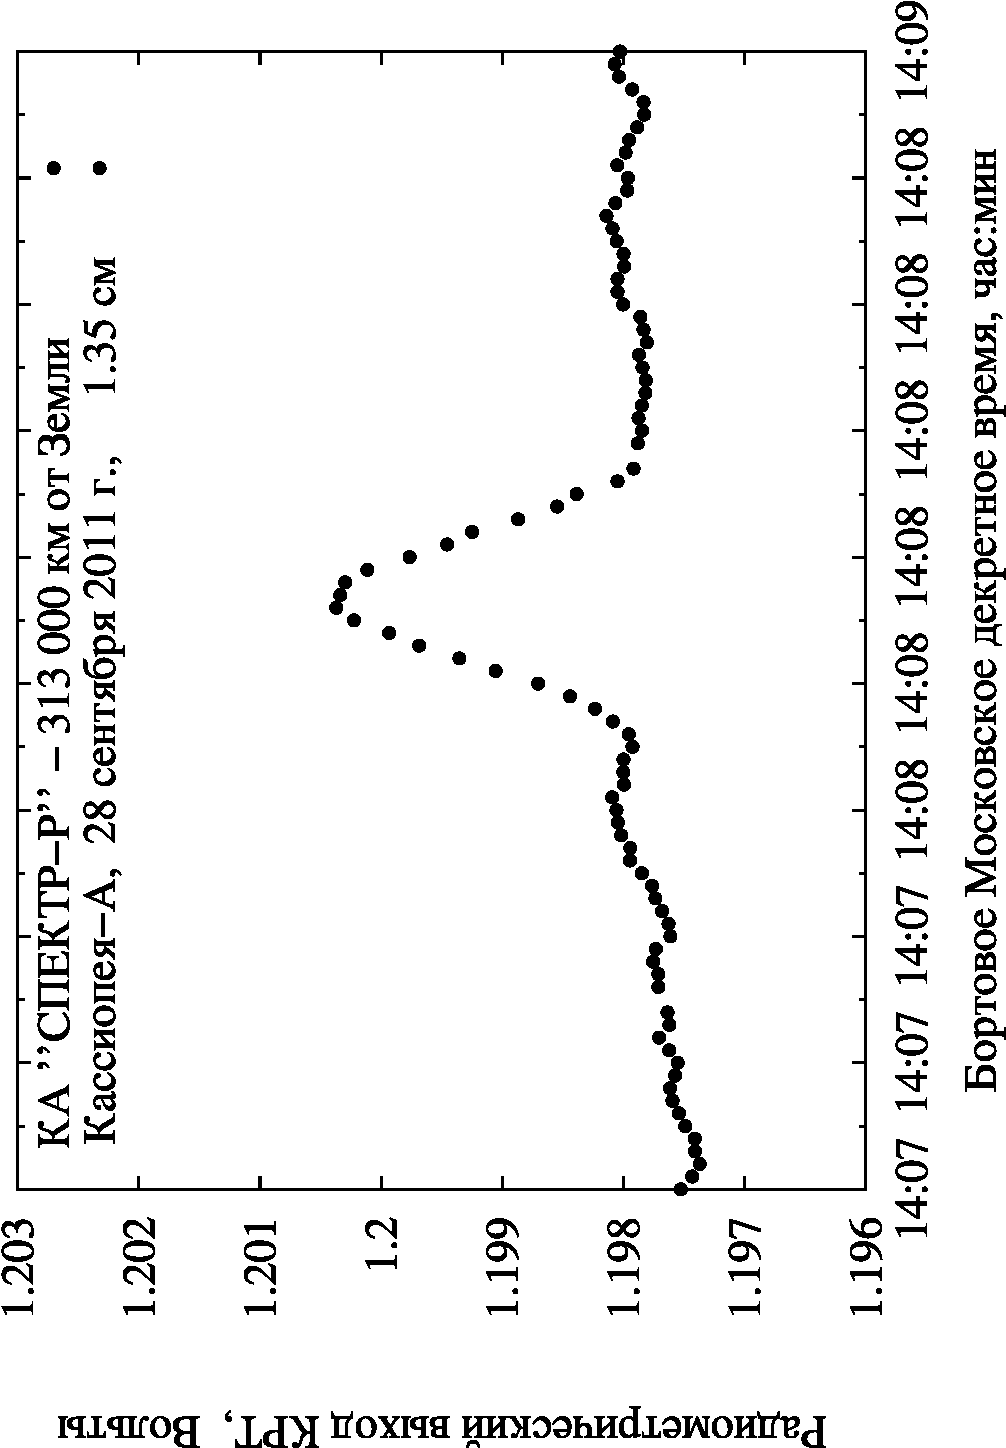
\includegraphics[width=0.3\textwidth,origin=c,angle=-90]{Fig8a_ru.pdf} \\
    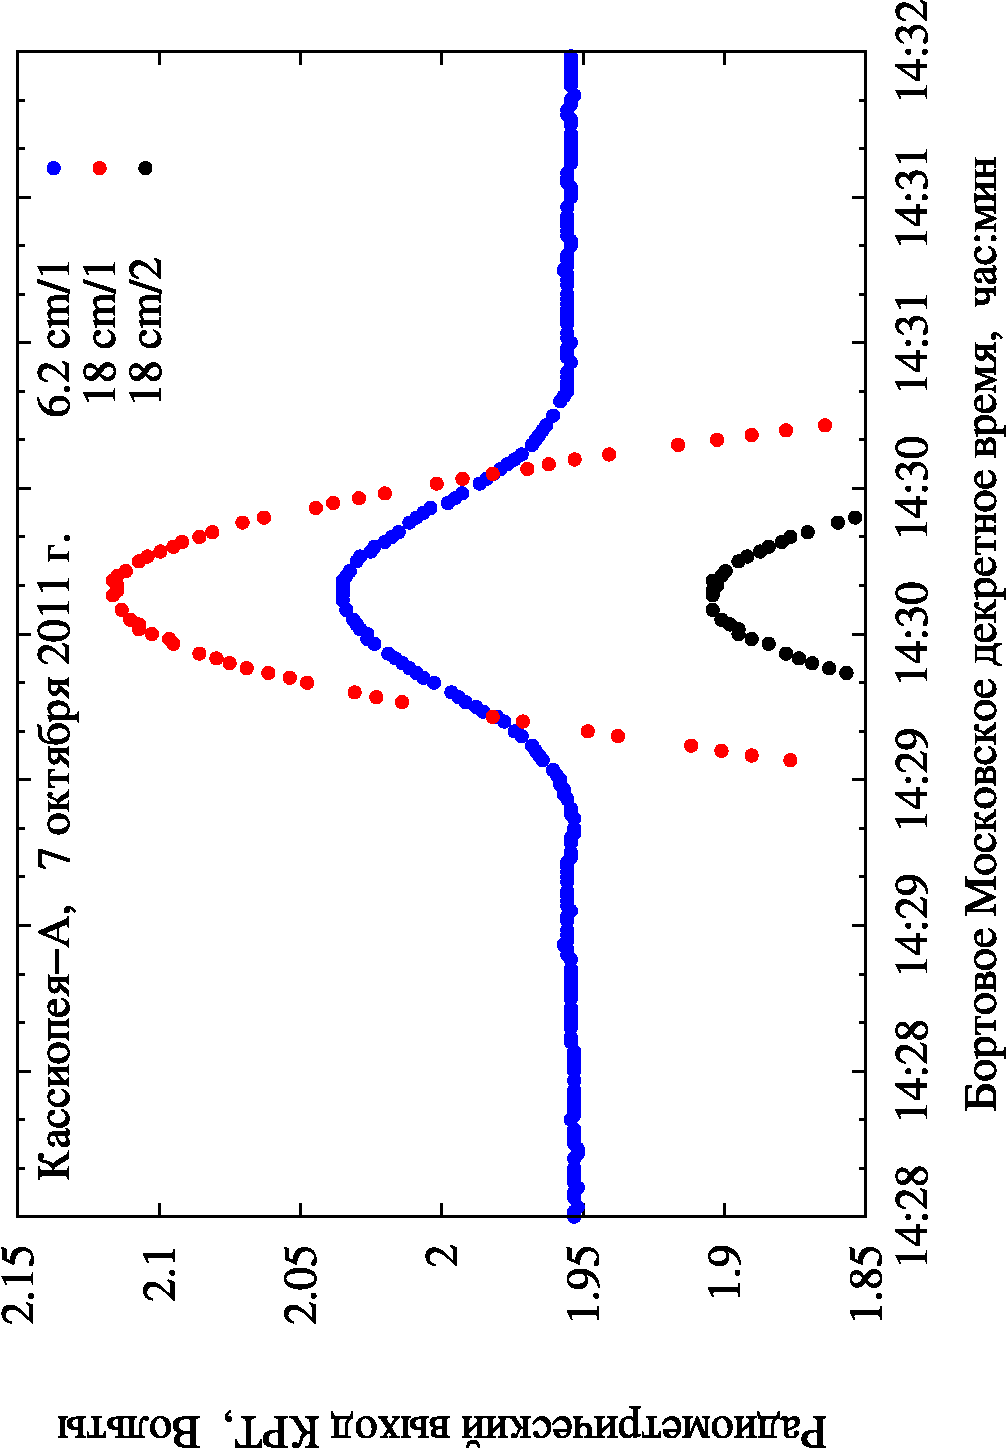
\includegraphics[width=0.3\textwidth,origin=c,angle=-90]{Fig8b_ru.pdf} \\
    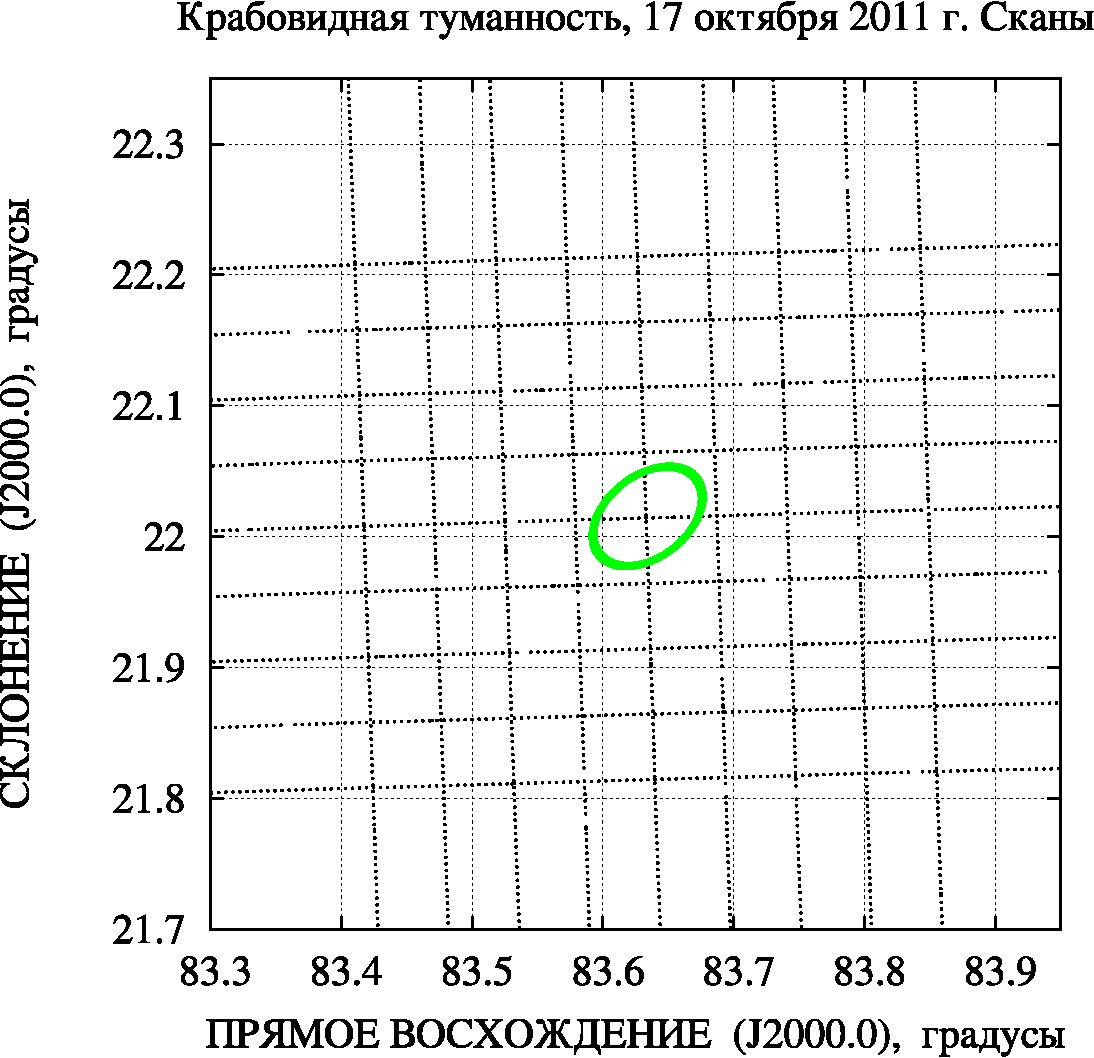
\includegraphics[width=0.3\textwidth,origin=c,angle=0]{Fig8c_ru.pdf}
 }
 \caption{Первый радиометрический отклик КРТ по наблюдениям Кассиопеи-А
в диапазоне 1.35 см 28 сентября 2011 г. (а)
и в диапазоне 6.2 см 7 октября 2011 г.
на фоне одновременных откликов в ортогональных поляризациях
на длине волны 18 см  (б).
Траектории сканирования участка неба с Крабовидной туманностью
17 октября 2011 г. (в), которым соответствуют отклики
сигналов в диапазонах 1.35 и 6.2 см, приведенные на графике 7б цветной вкладки.
Условный контур в центре характеризует угловые размеры
радиоисточника.}
\end{figure}

\begin{figure}
 \centerfloat{
    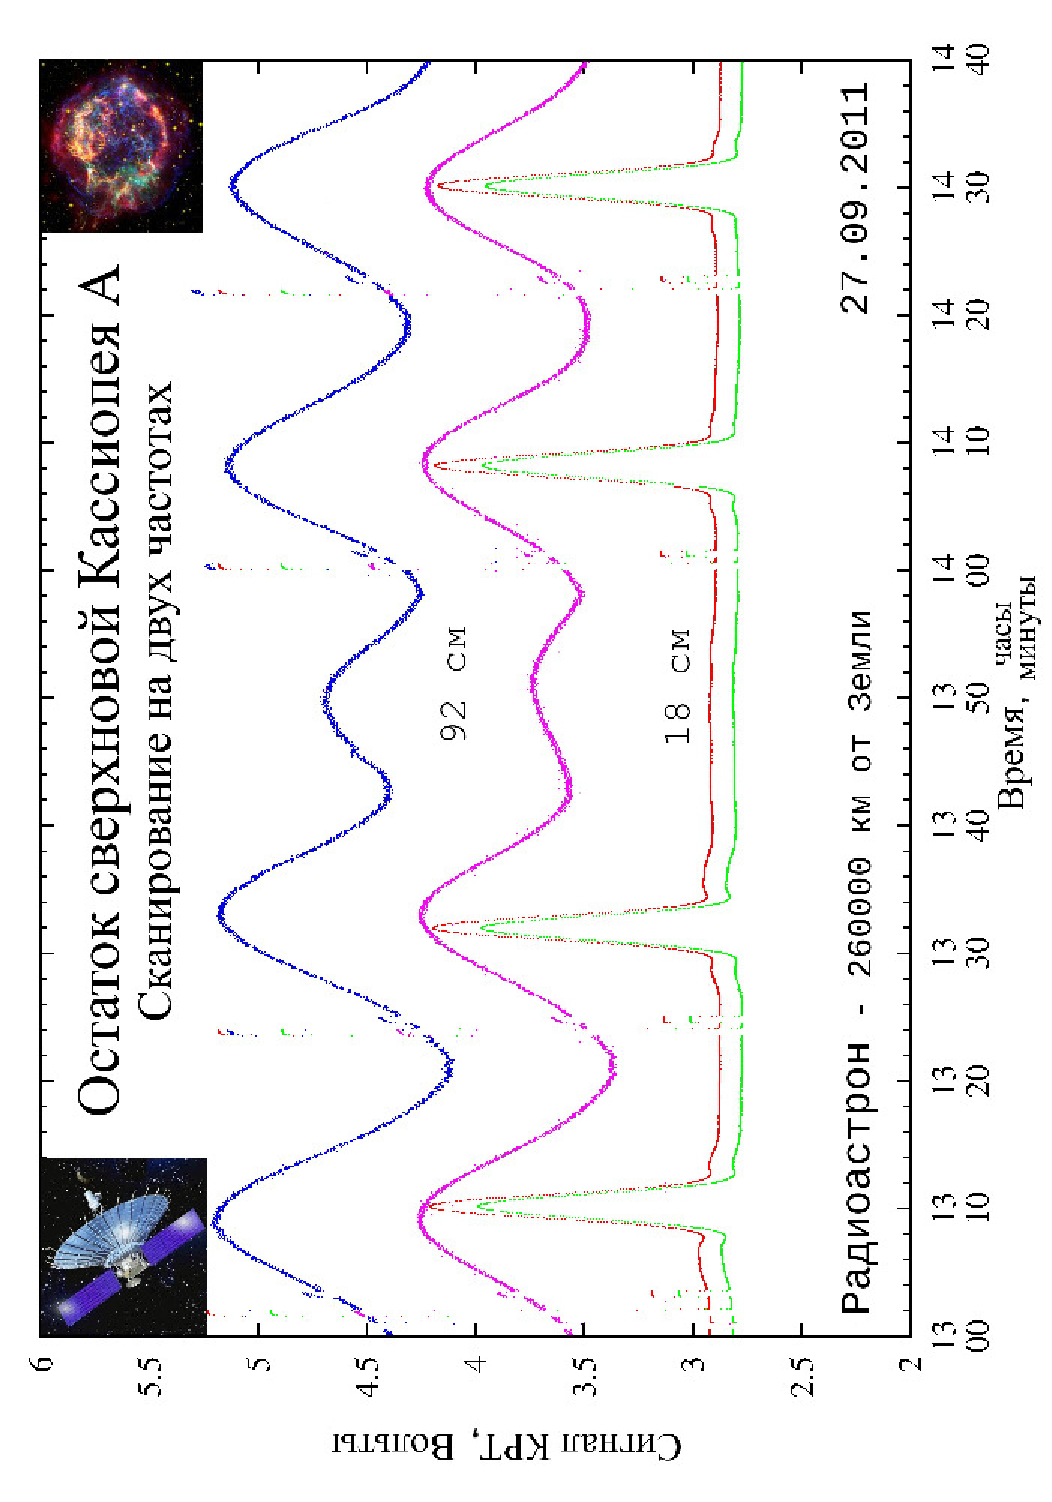
\includegraphics[width=0.3\textwidth,origin=c,angle=-90]{Fig7a_ru.pdf}
    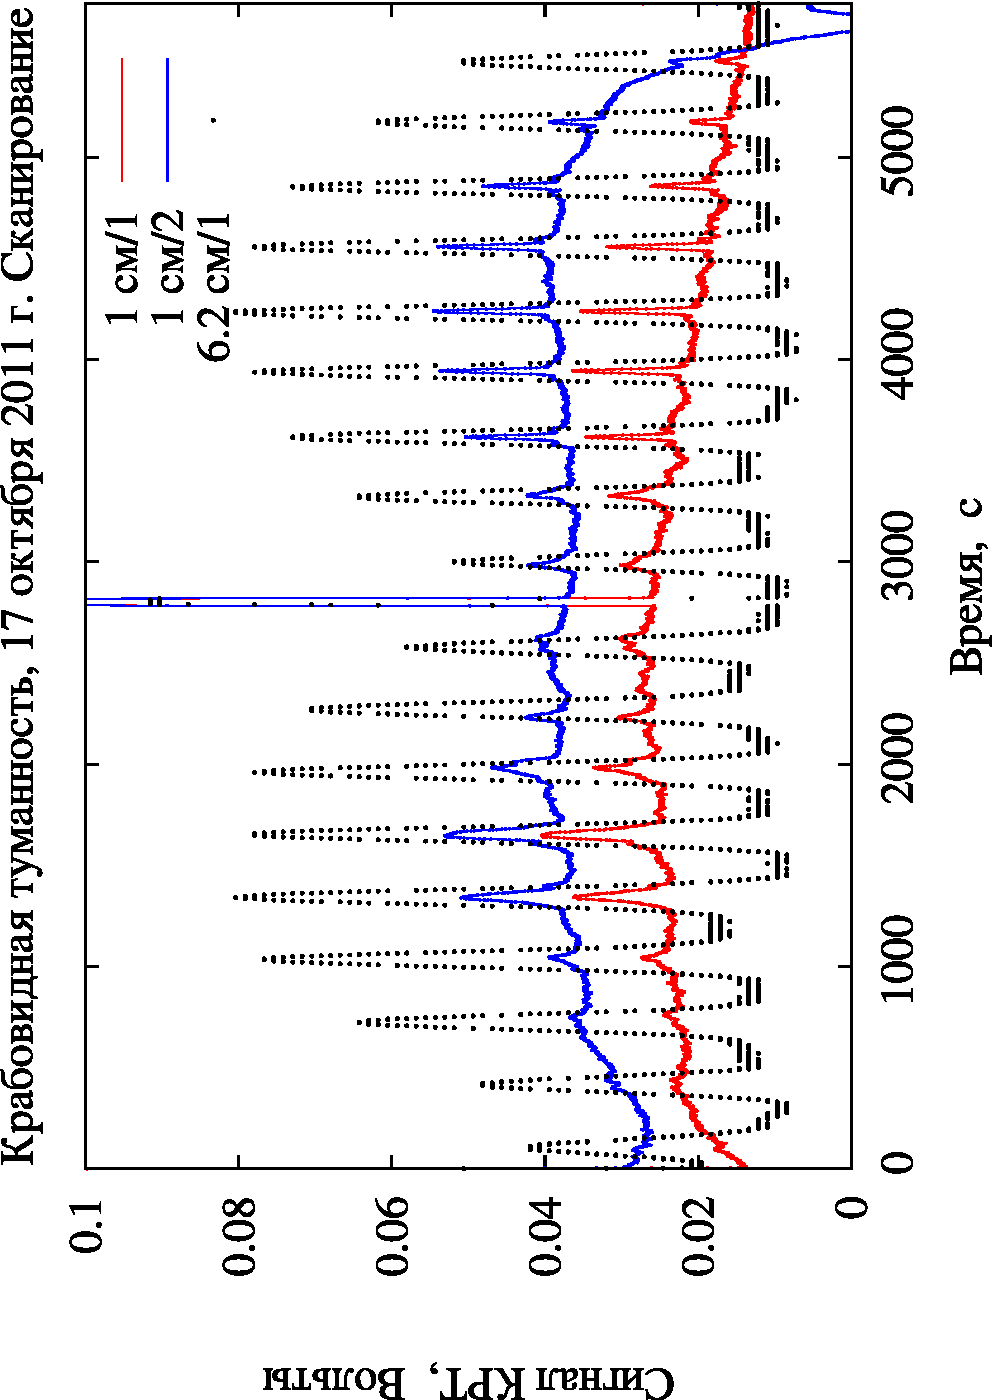
\includegraphics[width=0.3\textwidth,origin=c,angle=-90]{Fig7b_ru.pdf}
 }
 \caption{}
\end{figure}

\begin{figure}
 \centerfloat{
    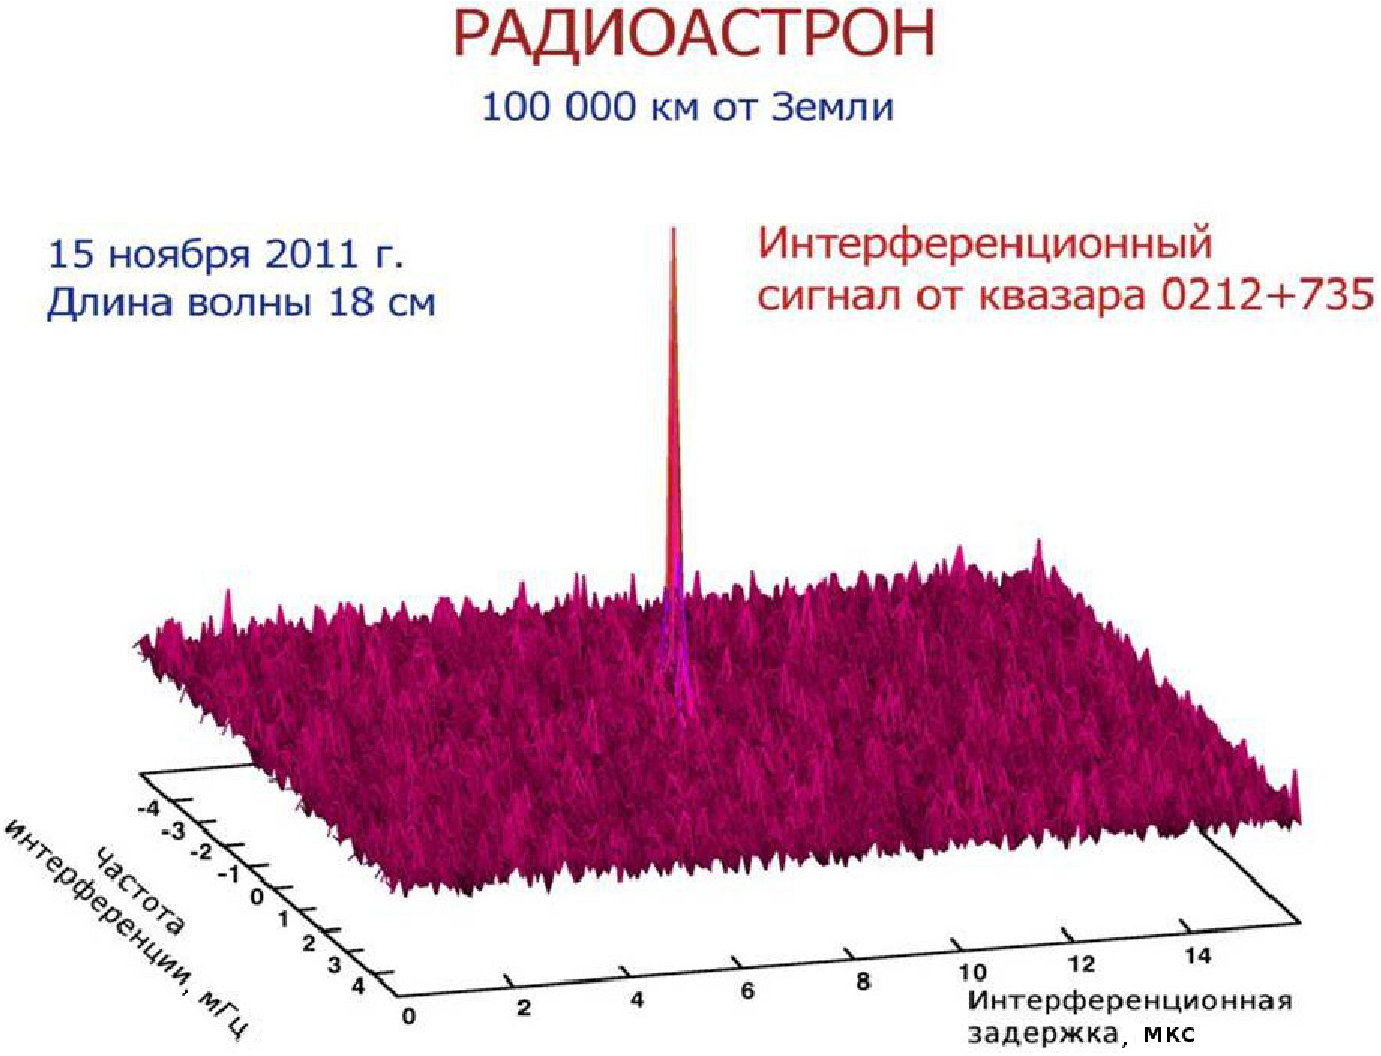
\includegraphics[width=0.4\textwidth]{Fig7c_ru.pdf} \hfill
    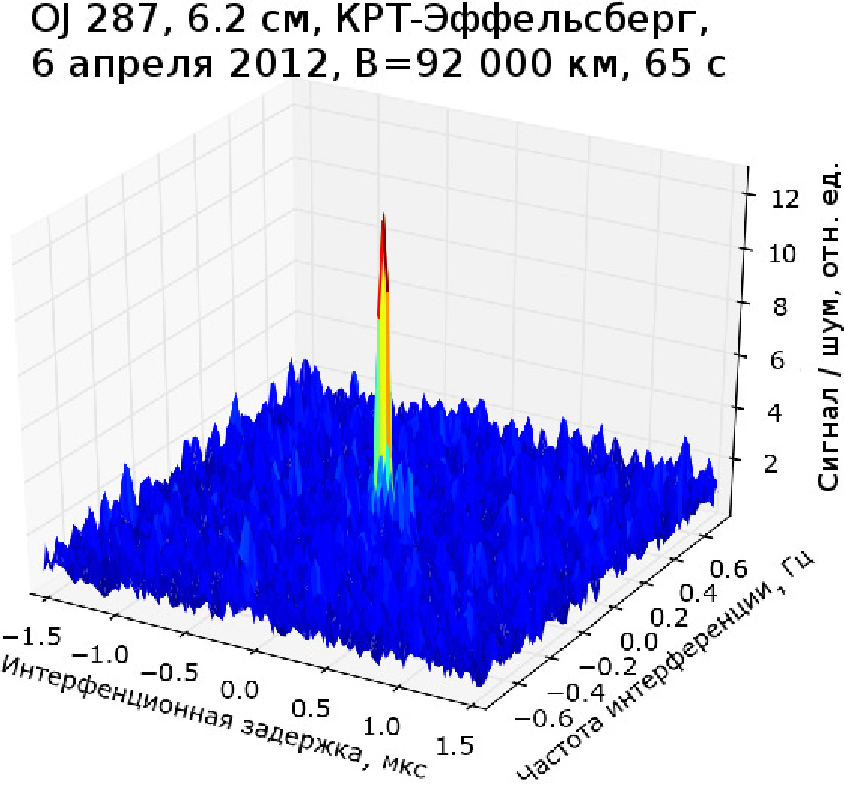
\includegraphics[width=0.4\textwidth]{Fig7d_ru.pdf}
 }
 \caption{}
\end{figure}

\begin{table}
\caption{Основные ожидаемые (1.1--1.10) и измеренные
(2.1--2.10) параметры КРТ в диапазонах длин волн K, C, L, P:
ширина главного лепестка диаграммы направленности по уровню
половинной мощности $\vartheta_{0.5}$ и $\varphi_{0.5}$,
эффективная площадь $A_{eff}$,
коэффициент использования площади КИП,
эффективная температура шума системы $T_{sys}$ и приемника
$T_{rec}$,
эффективная плотность потока излучения системы $F_{sys} \equiv$ SEFD,
систематическая ошибка при сканировании  $\Delta \vartheta_s$
по оси $\vartheta$ и $\Delta \varphi_s$ по оси $\varphi$
после ввода постоянной поправки $\delta \vartheta_p$ в
наведение телескопа,
чувствительность интерферометра $\sigma_{SVLBI}$,
отношение $\alpha_{D}$
измеренной ширины главного лепестка диаграммы направленности к его
идеальной ширине $\lambda / D$, где $D = 10$ м --- диаметр зеркала}
\bigskip
\label{tab:srt_params1}
\centering
    \begin{SingleSpace}
        \begin{tabular}{l|r|r|r|r}
        % \hline
        \toprule
        Параметр              &K($1.35$ см)&C($6.2$ см)&L($18$ см)&P($92$ см)\\
        \midrule
1.\quad  КРТ в Пущино, 2003--2004:& & & &\\
                                  & & & &\\
1.1\quad $\vartheta_{0.5} \pm 5\%$, \,\,\,\,\,\,\,\,\,
&  $5.6^\prime$ & $25.5^\prime$  & $74.5^\prime$ & $6.2^\circ$ \\
1.2\quad  $A_{eff} \pm 10\%$, \,\,\,\,  м$^2$     &   27 &   40 &   40 &  24\\
1.3\quad  КИП = $A_{eff}/A_{geom} \pm 10\%$ & 0.34 & 0.51 & 0.51 & 0.31\\
1.4\quad  $T_{sys}/T_{rec}$, \,\,\, K                                   &80/45 & 70/30 & 50/15
&140/30\\
1.5\quad  $T_{sys}^{(opt)}$, \,\,\, K                                    &70    & 66    &  33  &
164\\
1.6\quad  $SEFD_{srt}^{(opt)}$, \,\,\, Ян                                        &7200    &4600
&2300  &19000\\
1.7\quad  $SEFD_{GB}$, \,\,\, Ян                                         & 23     & 8     & 10   &
55\\
1.8\quad  $\Delta \nu_{IF}$, \,\,\, МГц                                   & 16     & 16    & 16   &
4\\
1.9\quad  $\sigma_{SVLBI}^{(opt)}$ (при $\Delta t = 5$ мин), \,\,\, мЯн  & 7   & 3   & 3   & 33\\
1.10\quad  $\alpha_D = \vartheta_{0.5} \cdot D / \lambda$\,\,\,                     & 1.21   & 1.20
& 1.20 & 1.18\\
%[4pt]
\hline
%[-6pt]
2.\quad  КРТ в полете, 2011--2012: & & & &\\
                       & & & &\\
2.1\quad  $(\vartheta_{0.5} \pm 5 \%)$ x $(\varphi_{0.5} \pm 5 \%)$,\,
& $6.0^\prime$ x $13^\prime$ & $25^\prime$    & $72^\prime$   & $6.1^\circ$ \\
2.2\quad  $A_{eff} \pm 13\%$, \,\,\, м$^2$;                            & 7.5       & 35    & 41   &
30\\
2.3\quad  КИП = $A_{eff}/A_{geom} \pm 13\%$                            & 0.1       & 0.45  & 0.52 &
0.38\\
2.4\quad  $T_{sys} \pm 13\%$, \,\,\,\,\, K                             & 77        & 130   & 45   &
200\\
2.5\quad  $F_{sys} \pm 10\%$\,\,(SEFD$_{srt})$, \,\,\, Ян              & 30000 & 10500 & 3400 &
19000\\
2.6\quad  $\vert \Delta \vartheta_s \vert$, \,\,\,\, &$1.2^\prime \pm 0.2^\prime$            & & &
\\
2.7\quad  $\vert \Delta \varphi_s \vert$, \,\,\,\,\, &$< 1.5^\prime$            & & & \\
2.8\quad  $\delta \vartheta_p$, \,\,\,\,\,           &$2.5^\prime$              & & & \\
2.9\quad  $\sigma_{SVLBI}$ (при $\Delta t = 5$ мин), \,\,\, мЯн        & 13        & 5     & 3    &
33\\
2.10\quad  $\alpha_D = (\vartheta_{0.5}\times \varphi_{0.5}) \cdot D / \lambda$ &$1.29 \times 2.80$
&1.17 &1.16 &1.16\\
        \bottomrule
        \end{tabular}
    \end{SingleSpace}
\end{table}


%\vspace{1cm}
%{\it 5.5. Результаты}
%\vspace{0.5cm}
\subsubsection{Результаты}


Основные результаты суммированы в табл.~2 (измерения), а также в табл.~3 (анализ измерений) в
Приложении. В табл.~2 включены также основные результаты наземных радиоастрономических испытаний
технологической модели КРТ на полигоне в Пущинской обсерватории АКЦ ФИАН, полученные в 2003--2004
гг. \cite{SRT_report_2004}. Типичные радиометрические отклики на примерах первых сканирований
показаны на рис. 7a (цветная вкладка), 8a и 8б для диапазонов 92, 18, 1.35 и 6.2 см по наблюдениям
Кассиопеи-А (первого из астрономических объектов, наблюдавшихся с космическим радиотелескопом с 27
сентября 2011 г.) и на рис. 7б (цветная вкладка) по наблюдениям Крабовидной туманности в диапазонах
1.35 и 6.2 см. Пример сканирования площадки неба дан на рис. 8в. Приведенным на нем траекториям
соответствуют радиометрические отклики на рис. 7б. Для антенных измерений использовались также
Юпитер, Луна и Дева-A (протяженные объекты) и квазиточечные внегалактические радиоисточники 3С\,84,
3С\,273 и 3С\,279.

Характеристики  стандартных калибраторов (потоки, распределение яркости, угловые размеры,
поляризация) брались из литературы \cite{Baars_1977}, а потоки сильных квазиточечных радиоисточников
3С\,84, 3С\,273 и 3С\,279, являющихся переменными, --- по измерениям на 600-м кольцевом
радиотелескопе РАТАН-600 САО РАН (Нижний Архыз, Россия) и на 100-м параболоиде в Эффельсберге
Института радиоастрономии им. Макса Планка (Бонн, ФРГ) \cite{FGAMMA} в близкие к бортовым
измерениям даты. Процедуру наземных измерений см. в \cite{Kovalev_1999}.


%{\it 5.6. Обсуждение результатов}
%\vspace{0.5cm}
\subsubsection{Обсуждение результатов}

Как известно, при отсутствии фазовых погрешностей, ширина $\vartheta_{0.5}$ главного лепестка
диаграммы направленности по половинной мощности и коэффициент использования площади $\eta$ (КИП),
равный отношению эффективной площади к геометрической, зависят от закона распределения амплитуды и
фазы электрического поля по раскрыву зеркала антенны и от уровня облучения края зеркала. Для
идеального параболического рефлектора с диаметром $D$ круглого раскрыва, при некоторых типовых
теоретических законах амплитудного распределения синфазного поля, ожидаемые ширина диаграммы
$\vartheta_{0.5}$ и КИП $\eta_0$ на длине волны $\lambda$ для синфазного случая могут быть оценены с
помощью соотношений \cite{Hansen_1966,Ajzenberg_1977,Christiansen_1972} $\vartheta_{0.5} = \alpha_D
\cdot \lambda / D$, где $\alpha_D \approx 1.0 \div 1.5$, и $\eta_0 \approx 1.0 \div 0.55$ в
зависимости от конкретого закона распределения поля. При этом, чем меньше уровень облучения края
зеркала, тем меньше $\eta_0$ (КИП) и больше $\alpha_D$ (шире диаграмма направленности), и они близки
к единице только при одинаковой амплитуде поля по раскрыву. Фазовые искажения синфазного поля в
раскрыве дополнительно увеличивают коэффициент $\alpha_D$ и уменьшают $\eta_0$, т.е. расширяют
главный лепесток диаграммы направленности и уменьшают эффективную площадь.

Сравнивая эти значения $\alpha_D$ с полученными $\alpha_D \approx 1.2$ по измерениям КРТ (см.
параметры 1.10 и 2.10 в табл. 2), видим, что для диапазонов 92, 18 и 6.2 см измеренная ширина
главного лепестка диаграммы направленности соответствует значениям, близким к теоретически
ожидаемым. Наиболее существенные отличия результатов измерений параметров КРТ в полете от параметров
проектных или ожидаемых, полученных ранее по испытаниям КРТ в Пущино \cite{SRT_report_2004},
относятся к эффективной площади и к форме главного лепестка диаграммы направленности в диапазоне
1.35 см, а также к температуре шумов КРТ в диапазоне 6.2 см (табл.~2). Для работы в режиме синтеза
широкой полосы частот в диапазоне 1.35 см предусмотрен выбор любой из 8 входных полос. Приведенные
результаты относятся к центральной полосе $F_0$ (см. раздел 2.2.2).

%\vspace{0.5cm}
%{\it 5.6.1. Диапазон 1.35 см (центральная полоса F0)}
%\vspace{0.5cm}
\paragraph{Диапазон 1.35 см (центральная полоса $F_0$)}

Измеренное в этом диапазоне поперечное сечение главного лепестка диаграммы направленности по уровню
половинной мощности представляет собой примерно эллипс с осями $\vartheta_{0.5}\times \varphi_{0.5}$
= $6.0^\prime\times 13^\prime$ при относительной ошибке 5\%, вместо ожидаемого круга диаметром
$(5.6^\prime \pm 10\%)$. Наглядно эта особенность хорошо видна по откликам на сканирование площадки
неба с источником (рис. 7б на цветной вкладке и рис. 8в). Измеренная эффективная площадь оказалась
равной $(7.5 \pm 13\%)$ м$^2$ вместо ожидаемого значения $(27 \pm 10\%)$ м$^2$ или хотя бы
проектного значения $(23 \pm 15\%)$ м$^2$. Эти ожидаемые значения для диаграммы и площади были
получены при наземных испытаниях КРТ в Пущино в 2004 г. Отличие полученной в наземных испытаниях
эффективной площади от эффективной площади идеальной параболической поверхности ($40 \div 45$ м$^2$)
естественно объяснялось влиянием случайной погрешности реализации поверхности зеркала, выполненной
со среднеквадратичным отклонением не хуже проектного значения $\sigma = 0.77$ мм, которое было
задано в проекте допуском $d = \pm 2$ мм ($\vert d \vert = 2.6 \sigma$ \cite{Esepkina_1973}). Этой
же причиной, но при $\sigma \approx 1.4$ мм, или другой типичной причиной (систематической
квадратичной фазовой погрешностью в раскрыве антенны, --- с максимальным значением $\sim 1.5\,\pi$;
см. Приложение) могло бы быть формально объяснено и уменьшение эффективной площади до 7.5 м$^2$,
если бы не наблюдаемое при этом существенное искажение формы главного лепестка диаграммы
направленности.

Искажения диаграммы направленности в параболических антеннах вызываются, в основном, тремя видами
систематических фазовых искажений амплитудно-фазового распределения поля в раскрыве зеркала
\cite{Hansen_1966,Ajzenberg_1977,Christiansen_1972,Galimov_2010}: квадратичными, кубическими (комой)
и астигматизмом зеркала и/или облучателя. За квадратичные и кубические искажения могут быть
ответственны как зеркало или облучатель, так и смещение облучателя из фокуса зеркала --- в
продольном (для квадратичных искажений) или поперечном (для комы) направлениях к оси параболоида.
Астигматизм является следствием того факта, что точки наилучшей фокусировки в двух главных
взаимно-ортогональных плоскостях, перпендикулярных раскрыву, не совпадают \cite{Hansen_1966}. Это
означает, что оптимальная точка фокусировки для облучателя, установленного в положение с
минимальными аберрациями (и соответственно --- с минимальной шириной главного лепестка диаграммы
направленности), различна в этих плоскостях --- в каждой из них своя точка, и единый фазовый центр
отсутствует. При этом обычно существует некоторый общий <<эквивалентный центр оптимальной
фокусировки>> или <<эквивалентный фазовый центр>> вблизи середины этих положений, при установке в
который фазовые аберрации и искажения диаграммы направленности удается минимизировать
\cite{Hansen_1966,Galimov_2010}. Фазовые погрешности в раскрыве есть сумма всех погрешностей,
обусловленных зеркалом, облучателем и смещением облучателя из фокуса зеркала
\cite{Shubarin_1960,Cejtlin_1976}. Поэтому однозначно установить реальную причину фазовых искажений
в раскрыве антенны только по результатам летных испытаний, без дополнительных данных или
предположений, не представляется возможным.

Как свидетельствует подробный анализ проблемы (см. Приложение), наблюдаемую эллиптичность главного
лепестка диаграммы направленности, как и измеренное значение эффективной площади, в диапазоне 1.35
см проще всего объяснить, предположив систематическую квадратичную погрешность в распределении фазы
по оси $\varphi$ порядка $1.5 \pi$ в раскрыве антенны и астигматизм, обусловленные облучателем,
дополнительно к случайной погрешности реализации параболической поверхности зеркала КРТ с проектным
значением среднеквадратичного отклонения $\sigma = 0.77$ мм, использованным выше. Такая
систематическая фазовая погрешность по одной оси в раскрыве могла бы, например, возникать при
астигматизме облучателя с квадратичной фазовой погрешностью и одновременном смещении центра
оптимальной фокусировки облучателя относительно фокуса зеркала на величину порядка 0.3 см вдоль оси
параболоида, при расстоянии $b \sim 2$ см между двумя такими центрами фокусировки облучателя. В
пользу этого предположения свидетельствуют результаты оценок в одной из моделей фазовых искажений в
Приложении, использующей результаты численного расчета \cite{}  амплитудно-фазовой диаграммы
направленности БАО. Расчет \cite{} указывает на возможность астигматизма и квадратичных аберраций
облучения зеркала со значениями, близкими к необходимым для объяснения результатов измерений в
диапазоне 1.35 см.

Предпринятые попытки (см. Приложение) дать согласованное аргументированное объяснение всей
совокупности антенных измерений без астигматизма облучателя в этом диапазоне успеха не имели. Но это
только одно из возможных объяснений. Формально можно также предположить, что полученные
систематические фазовые погрешности в раскрыве вызваны не облучателем, а зеркалом антенны. Однако
для такого вывода в настоящий момент нет достаточных оснований и данных для количественного анализа.
Простой близкий вариант для объяснения асимметрии диаграммы направленности --- гипотеза о
соответствующей сильной асимметричной деформации зеркала --- так, чтобы размер раскрыва антенны в
одной из плоскостей уменьшился примерно вдвое (до 5 м), должен был бы сказаться на результатах во
всех диапазонах. А это противоречит <<хорошим>> результатам антенных измерений в диапазонах 6.2, 18
и 92 см, которые близки к проектным.

%\vspace{0.5cm}
%{\it 5.6.2. Диапазоны 6 см, 18 см и 92 см}
%\vspace{0.5cm}
\paragraph{Диапазоны 6.2, 18 и 92 см}

В отличие от других диапазонов все измерения в диапазоне 6.2 см проведены при раздельной работе с
поляризационными каналами. Одновременное их включение сразу приводило к зашкалу выходных сигналов,
которое не устранялось аттенюаторами. Зарегистрированы также искажения автоспектра выходных
видеополос для канала с правой поляризацией в интерферометрическом режиме. Эти факты позволяют
предположить, что на участке <<вход БАО--вход МШУ>> антенно-фидерного тракта в диапазоне 6.2 см
ухудшилось согласование поляризационных каналов БАО со свободным пространством и/или с МШУ и
ухудшилась развязка между каналами. Это привело к увеличению реактивных и активных потерь на этом
участке при раздельном включении каналов и, как следствие, к увеличению шумовой температуры системы
согласно (5.7), а также к самовозбуждению МШУ при одновременной работе каналов. Исследование
продолжается.

Во всех антенных измерениях использовались предварительные значения антенной температуры $T_{NS}$
ГШ, полученные по результатам предполетных наземных измерений и <<пересчета>> $T_{NS}$ ко входу КРТ
согласно формуле (5.7в) по измеренным или рассчитанным потерям  \cite{RAUH} в антенно-фидерном
тракте. Планировалась их коррекция по результатам летных испытаний. Коррекция для диапазонов 92, 18
и 1.35 см не проводилась. Коррекция $T_{NS}$ ГШ для диапазона 6.2 см проведена: 1) в предположении
соответствующего увеличения потерь в БАО (т.е. уменьшения $K_2$ в соотношениях (5.7б), (5.7в)) и 2)
в пренебрежении искажениями от диаграммы направленности облучателя, уменьшающими эффективную
площадь, что не противоречит результатам расчета  \cite{} и оценкам параметров 4.2 и 5.2 в табл.~3
для этого диапазона\footnote {Так как в блоке антенных облучателей (БАО) конструктивно объединены
облучатели с полосковыми или волноводными формирователями левой и правой круговых поляризаций для
каждого дипапазона (см. разделы 5.1 и  2), то потери в БАО характеризуют не только потери в самих
облучателях (в основном, на высшие типы волн), но и в следующих за ними поляризаторах. }. Эта
коррекция привела к соответствующему увеличению полученных значений эффективной площади $A_{eff}$ и
эквивалентной шумовой температуры системы $T_{sys}$ в диапазоне 6.2 см (т.е. к <<улучшению>>
$A_{eff}$ и <<ухудшению>> $T_{sys}$).

Она же  позволила дать общее согласованное объяснение измеренной зависимости эффективной площади КРТ
от длины волны во всех диапазонах с помощью единого подхода к учету фазовых погрешностей. И
одновременно --- объяснить соответствующее повышение шумовой температуры системы согласно (5.7)  в
диапазоне 6.2 см и, возможно, частично, в диапазоне 92 см: увеличением потерь $L_2$ в БАО
относительно проектных значений\footnote {Из-за недостатка средств  и известных технических проблем
калибровки антенных измерений, в том числе и проблем изготовления высококачественных апертурных
охлаждаемых согласованных нагрузок, проектная документация содержит только расчетное значение потерь
БАО в диапазоне 92 см и результаты косвенных лабораторных измерений  или теоретических оценок таких
потерь в остальных диапазонах.}. Для шумовой температуры КРТ в диапазоне 92 см существенен также
вклад от фонового излучения неба, который, кроме того, может заметно меняться с изменением
направления на объект и полностью или частично объяснять 20-процентное превышение измеренной
температуры шумов КРТ $T_{sys} = 200$ К над ожидаемой. Минимальный вклад фона неба при антенне,
направленной в полюс Галактики, по оценкам, использующим опубликованные распределения яркостной
температуры неба и соотношения (5.7), (5.7а), составляет около 60 К, который включен в ожидаемую
температуру $T_{sys}^{(opt)} = 164 $ К \cite{RAUH}.

Стоит подчеркнуть, что потери $L_2 = 1 / K_2$ БАО входят в 3 слагаемых в (5.7), что не всегда
принимается во внимание при грубых оценках. Заметим также, что, в отличие от калибровки по антенной
температуре, необходимой для антенных измерений, обычно используемая в астрономических измерениях
<<астрономическая калибровка>> наземных радиотелескопов и КРТ, --- в единицах эквивалентной
спектральной плотности потока излучения для системы с помощью $F_{sys}$ (SEFD) и для генератора шума
ГШ  с помощью $F_{NS}$,   --- не зависит от этих особенностей и коррекций, так как пропорциональна
$T_{sys}/A_{eff}$ (для SEFD) или $T_{NS} / A_{eff}$ (для $F_{NS}$), и может выполняться по
астрономическим источникам радиоизлучения без знания абсолютных величин антенной температуры
$T_{NS}$ ГШ и $T_{sys}$ системы (см. раздел 5.1 и \cite{Kovalev_1999}).

%\vspace{0.5cm}
%{\it 5.6.3. Поправки наведения и сканирования}
%\vspace{0.5cm}
\paragraph{Поправки наведения и сканирования}

Поправки измерялись при сканировании площадки с источником
по осям $\vartheta$ и $\varphi$ (см. пример на рис. 7б на цветной вкладке и рис. 8в).
По результатам такого сканирования находились центральные
сечения источника, для которых процесс сканирования многократно
повторялся в прямом и обратном направлениях движения по каждой оси.
Используя телеметрические данные штатного координатного обеспечения,
отдельно для прямого и для обратного направлений сканы
усреднялись, и вычислялась разность координат между расчетным и
измеренным положениями максимума сигнала, которая и определяла
искомые поправки к расчетным координатам.

Измеренная величина погрешности координат по оси $\vartheta$ (с меньшей шириной
диаграммы направленности, равной $\vartheta_{0.5} = 6^\prime$)
при сканировании <<вперед>> систематически отличается от величины
при сканировании <<назад>>, а кривая сканирования имеет характерный для наземных
телескопов <<двугорбый>> вид  со значениями, равными $(3.7^\prime \pm 0.2^\prime)$
для одного максимума и $ 1.3^\prime \pm 0.2^\prime $    для другого максимума.
По этим данным введена постоянная поправка в наведение
$\Delta \vartheta_p = 2.5^\prime$,
равная среднему значению между ними, с которой далее  работали постоянно.
"Двугорбость>> при сканировании в противоположных направлениях сохранялась,
--- примерно с прежним запаздыванием, соответствующим
$\vert \Delta \vartheta_s \vert = 1.2^\prime \pm 0.2^\prime$ к расчетному значению, ---
всегда с запаздыванием по времени, независимо от прямого или обратного
направления сканирования, но уже относительно нулевого среднего значения
между максимумами. Такое запаздывание электрической оси при движении КРТ
относительно нового расчетного положения оси мы интерпретировали как
систематическую ошибку сканирования (табл.~2).
По другой оси поправка не вводилась, так как результаты
были в пределах ошибок измерений.

Примерно половина измеренного интервала времени между <<горбами>> может объясняться эффектом
задержки отклика при интегрировании сигнала на радиометрическом выходе (см. об этом эффекте в
\cite{Kuzmin_1964}). Считается, что основная причина двугорбой кривой для наземных телескопов
(отсутствующая для КРТ) --- люфты в механизмах управления. Причина аналогичного поведения КРТ может
быть связана с подобными задержками при интегрировании сигналов в электронике систем звездных
датчиков и цепях управления движением космического аппарата или с другими причинами и нуждается в
дополнительном изучении. Гипотезе об упругих деформациях штанг, на которых крепится фокальный
контейнер КРТ, противоречат результаты анализа телеметрии, свидетельствующие о достаточно
равномерной скорости на участках движения.

%\vspace{0.5cm}
%{\it 5.6.4. Шум телеметрии}
%\vspace{0.5cm}
\paragraph{Шум телеметрии}

Анализ телеметрических данных показал наличие дополнительного
<<шума телеметрии>> для цифровых радиометрических выходов в обоих каналах
приемников диапазонов 18 и 92 см.
Он имеет вид фона, состоящего из <<пачек>> коротких импульсных
выбросов, и характерен для ошибок регистрации отдельных бит: амплитуда их
<<переменности>> не случайна, а систематически повторяется, изменяясь дискретно
от <<пачки к пачке>>. Сравнение с телеметрируемым параметром приемников <<АЦП готов>>
позволяет предположить, что этот шум вызван тем, что штатная телеметрическая система,
осуществляя опрос всех датчиков с фиксированной скоростью, не учитывает сигнал
готовности аналого-цифрового преобразователя (АЦП) в приемниках.
В результате опрос цифровых датчиков иногда осуществляется быстрее
реальной готовности АЦП в этих приборах. Впервые такой шум был обнаружен в
процессе приемо-сдаточных испытаний. Был найден и применен простой и эффективный
способ фильтрации, использование которого позволило устранить эту проблему
и в антенных измерениях КРТ в полете. В аналоговых выходах этих диапазонов
и во всех выходах приемников двух других диапазонов такой шум отсутствует.


\subsubsection{Выводы}

1. Полученная эквивалентная температура шума системы КРТ в пределах 20\%
совпадает с теоретическими оценкам в диапазонах 92, 18 и 1.35 см,
но вдвое превышает расчетное значение в диапазоне 6.2 см, что
в $\sqrt 2$ раз снижает ожидавшуюся для этого диапазона
чувствительность интерферометра (при фиксированном времени накопления).
Причиной такого повышения температуры шума, вероятно, является увеличение потерь в
антенно-фидерном тракте (скорее всего, на участке от БАО до МШУ) по сравнению с
потерями, рассчитанными на основе лабораторных измерений, выполненных на Земле.


2. Ширина главного лепестка диграммы направленности КРТ по уровню половинной мощности
в пределах погрешности близка к теоретически ожидаемым
и измеренным в наземных испытаниях значениям в
диапазонах 92, 18 и 6.2 см,
но заметно отличается от таковых в диапазоне 1.35 см:
поперечное сечение главного лепестка по уровню половинной мощности
на длине волны 1.35 см близко к эллиптическому с осями
$\vartheta_{0.5} \approx 6.0^\prime \pm 5\%$ и
$\varphi_{0.5} \approx 13 ^\prime  \pm 5\%$
 вместо проектной окружности диаметром $5.5 ^\prime  \pm 10\%$.
При этом профиль продольного сечения главного лепестка в той плоскости,
где он шире, заметно асимметричен.

3. Эффективная площадь КРТ в полете близка к расчетной или измеренной в наземных
испытаниях в диапазонах 92, 18 и 6.2 см.
В диапазоне 1.35 см она меньше ожидаемой по наземным измерениям площади
($27 \pm 10\%$) м$^2$ в 3.6 раза и проектной площади ($23 \pm 15\%$) м$^2$ ---
втрое, что почти в 2 раза уменьшает ожидаемую чувствительность в
интерферометрическом режиме (при фиксированном времени накопления).

4. Оценки, выполненные на основе расчетных значений амплитудно-фазовой диаграммы
направленности блока антенных облучателей  и простой модели фазовых погрешностей
в антенно-фидерной системе, приводят к следующим выводам о КРТ в полете:

--- средний профиль поверхности зеркала антенны может быть близким к
 параболическому с проектным значением  среднеквадратичного отклонения
 реальной поверхности зеркала от средней, равным 0.77 мм;

---  облучатель антенны может иметь:
а) квадратичные фазовые погрешности с максимальным значением
погрешности фазы облучения края зеркала, равным примерно $-100^\circ$ в
диапазоне 1.35 см и $-35^\circ$ в диапазонах 6.2 и 18 см
(согласно расчетным значениям фазовой диаграммы направленности
этих облучателей);
б) астигматические аберрации в диапазоне 1.35 см, аппроксимируемые
двумя эквивалентными центрами фокусировки облучателя, --- центрами 1 и 2
в ортогональных плоскостях 1 и 2, соответственно,---
вынесенными из фокуса зеркала примерно на 7 мм к зеркалу в
плоскости 1 и на 13 мм от зеркала в плоскости 2;
в) общий центр оптимальной фокусировки облучателя
(середина между центрами 1 и 2), который вынесен из фокуса
раскрывшейся антенны примерно на 3 мм от
зеркала в продольном направлении оси антенны;

--- эти фазовые погрешности облучения поверхности зеркала антенны
могут быть основными причинами измеренного уменьшения эффективной
площади и эллиптичности главного лепестка диаграммы направленности
КРТ в диапазоне 1.35 см  относительно проектных значений.

5. По результатам радиоюстировки средние погрешности наведения по
одной оси (с меньшей шириной главного лепестка диаграммы направленности
КРТ) составили $3.7^\prime \pm 0.2^\prime$  при
сканировании источника в одном направлении и $1.3^\prime \pm 0.2^\prime$  при сканировании в
противоположном направлении.
Частично этот результат может объясняться эффектом запаздывания отклика
из-за интегрирования
сигнала на радиометрическом выходе и нуждается в дополнительном изучении.
По этим измерениям введена постоянная поправка наведения
$\Delta \vartheta_p = 2.5^\prime$,
с которой далее работали постоянно. Оставшаяся погрешность сканирования
$\vert \Delta \vartheta_s \vert = 1.2^\prime \pm 0.2^\prime$   характеризует
запаздывание максимума сигнала относительно его расчетного
положения при сканировании в любом направлении и вызвана систематичеcкой
погрешностью при движении антенны.
По другой оси (с большей шириной главного лепестка диаграммы) погрешность
наведения лежит в пределах точности измерений, не превышая $1.5^\prime$,
и не компенсировалась в дальнейших наблюдениях.

6. Сравнение автокорреляционных спектров двух сильных мазерных источников в
диапазонах L и K позволяет сделать вывод о штатном функционировании спектрального
режима наблюдений космическим радиотелескопом и позволяет контролировать
частотные настройки и режимы поляризации при наблюдениях. Оценки чувствительности
КРТ, проведенные в рамках наблюдений спектральных радиолиний, согласуются
с данными исследований по источникам непрерывного спектра.
Незавершенной остается задача полного определения поляризационных параметров
радиотелескопа, что возможно при специально запланированных наблюдениях нескольких
ярких источников мазерного излучения, в частности, Orion KL.


\subsection{ПРОВЕРКА ФУНКЦИОНИРОВАНИЯ НАЗЕМНО-КОСМИЧЕСКОГО
         ИНТЕРФЕРОМЕТРА (ПЕРВЫЕ ЛЕПЕСТКИ) И ПЕРВЫЕ РЕЗУЛЬТАТЫ
         НАБЛЮДЕНИЙ}

В данном разделе представлен краткий обзор первых результатов,
полученных в интерферометрическом режиме. Эти результаты
будут подробнее обсуждаться в отдельных статьях позднее,
международными группами по поиску лепестков и Ранней научной
программе после завершения всестороннего анализа.

Детектирование интерференционного сигнала между космической обсерваторией
<<РадиоАстрон>>
и наземными радиотелескопами продемонстрировало общую успешную работу
комплексной РСДБ системы <<Космос--Земля>> во всех четырех диапазонах длин волн:
92, 18, 6.2 и 1.35 см (рис. 7в--7ж на цветной вкладке).
Первый сигнал космического
интерферометра был получен по наблюдениям 15 ноября 2011 г. квазара 0212+735 в
диапазоне 18 см при удалении КА от Земли, составившим около 100 000 км,
и проекции базы <<РадиоАстрон>> -- 100-м радиотелескоп в Эффельсберге
(Германия) на картинную плоскость источника $B = 8100$ км (рис. 7в на цветной вкладке).
Всего ко времени написания статьи проведено 20 сеансов испытаний интерферометра.
На рекордном удалении КА в 300 000 км (проекция базы составила
около 220 000 км) 25 января 2012 г. были проведены интерферометрические
наблюдения пульсара PSR 0950+08 в диапазоне 92 см с участием самого крупного
наземного радиотелескопа диаметром 300 м в обсерватории Аресибо (США) (рис. 7е, 7ж на цветной
вкладке).
Большинство
интерферометрических наблюдений проводилось в режиме c бортовым водородным
мазером, но были выполнены и успешные сеансы испытаний интерферометра в режиме
передачи на космический аппарат когерентного сигнала от водородного стандарта
Станции слежения в Пущино с обратной передачей его с аппарата на Станцию слежения
(так называемый <<режим замкнутой фазовой петли>>).

В режиме интерферометра чувствительность системы двух телескопов
пропорциональна квадратному корню из произведения эффективной
площади этих телескопов, и, таким образом, сочетание 10-м КРТ со 100-м
наземным радиотелескопом становится эквивалентным по чувствительности
системе двух 30-м телескопов. Режим наземно-космического
интерферометра не позволяет
получать результат исследования сразу после проведения измерений.
Зарегистрированные на различных радиотелескопах научные данные
передаются в центр обработки для первичной корреляции (обнаружения
интерферометрического отклика). Эта первичная корреляция может быть
выполнена только после высокоточной реконструкции орбиты КА в
баллистическом центре.

Обработка и анализ результатов, полученных на наземно-космическом интерферометре <<РадиоАстрон>>,
производится в АКЦ ФИАН совместно с другими участниками проекта. Здесь, в первую очередь,
выполняется кросс-корреляционная обработка потоков данных, записанных на отдельных радиотелескопах с
плотностью записи 128 или 256 Мбит/с, включая космический сегмент КРТ (128 Мбит/с), с помощью
созданной в АКЦ ФИАН системы регистрации РДР-1 \cite{Belousov_2007} и регистратора Mark5
\cite{Whitney_2003} разработки США. Программный FX-коррелятор АКЦ ФИАН построен на базе
вычислительного кластера с производительностью 1 Тфлоп/с и RAID-системой хранения информации
емкостью до 220 Тбайт. Технические характеристики процессорного кластера ЦОНИ АКЦ ФИАН позволяют
принимать поток данных от 10 станций, включая КРТ, с интегральной скоростью до 2.56 Гбит/с и,
соответственно, обрабатывать потоки до 45 формируемых в эксперименте баз интерферометров. Это может
выполняться практически без снижения темпа записанных в реальном времени и сохраненных в ЦОНИ данных
наблюдений.

Само по себе обнаружение интерферометрического отклика ещё не является окончательным результатом
научного исследования. Однако, при определенных предположениях о структуре компактной детали, оно
позволяет оценить ее угловой размер и яркостную температуру. Для достоверного заключения о строении
исследуемого объекта необходимы многократные наблюдения с различными конфигурациями телескопов и,
прежде всего, --- при разных положениях космического аппарата на его орбите. Необходимый набор таких
конфигураций может быть реализован как минимум в течение одного календарного года. Стратегия
наблюдений состоит в исследовании определенной выборки радиоисточников в течение целого года (а
иногда и нескольких лет), после чего всесторонний анализ дает возможность сделать обоснованные
заключения о структуре и физических условиях в изучаемых космических объектах.

Ранняя научная программа <<РадиоАстрон>> курируется АКЦ ФИАН и проводится с февраля 2012 г.
международными коллективами исследователей, сформированными в рамках проекта. К настоящему времени
измерены интерферометрические отклики от пульсаров PSR 0950+08, PSR 0531+21 (Crab) и PSR 0833-45
(Vela), PSR 1919+21, от активных ядер галактик 0212+735, 0716+714, 0748+126, 0754+100, 2013+370,
0851+202 (OJ287), 1954+513, 2200+420 (BL Lac), от галактического мазера W51 (см. Информационные
сообщения проекта <<РадиоАстрон>> за 2011--2012 гг. \cite{RA_news}). Эти отклики получены для
проекций базы наземно-космического интерферометра на картинную плоскость исследуемого источника
размерами от менее 10 000 км до около 250 000 км, т.е. примерно до 20 диаметров Земли.

14 ноября 2011 г., после подтверждения наблюдаемости на КРТ гигантских радиоимпульсов от пульсара в
Крабовидной туманности (расстояние 1 кпк), в диапазоне 18~см была впервые найдена корреляция между
этими импульсами, зарегистрированными КРТ и наземными радиотелескопами в Евпатории и обсерваториях
<<Светлое>>, <<Зеленчукская>> и <<Бадары>> ИПА РАН при проекциях базы интерферометров на картинную
плоскость источника до $B = 40 000$ км (рис. 10). Этот факт свидетельствует о том, что рассеяния
изображения в межзвездной среде от пульсара до наблюдателя на длине волны 18 см было не более
углового разрешения интерферометра, которое составило 400 мксек. дуги.

Интерферометрические наблюдения обычных импульсов близкого (260 пк) пульсара PSR 0950+08 (рис. 7е на
цветной вкладке) не обнаружили межзвездного рассеяния изображения даже в диапазоне 92 см при
проекции базы интерферометра вплоть до $B=220 000$ км. Тем самым впервые практически в метровом
диапазоне длин волн достигнуто угловое разрешение в  370 мксек. дуги. Наблюдения того же пульсара в
течении 1 ч (рис. 7ж на цветной вкладке) позволили впервые обнаружить переменность функции видности
интерферометра при столь больших базах интерферометра, что открывает путь к изучению параметров
турбулентности межзвездной плазмы и достижению еще более высокого углового разрешения источника с
использованием принципа <<межзёздного интерферометра>> \cite{Wolszczan_1987}. Для другого близкого
пульсара Vela, расстояние до которого $\sim 300$ пк, рассеяние в межзвездной среде было
зафиксировано. В мае 2012~г. крупнейшие радиотелескопы южного полушария провели совместно с КРТ
наблюдения этого пульсара на волне 18 см. В этих наблюдениях участвовали радиотелескопы обсерваторий
Паркс, Мопра, Хоббарт (все Австралия) и Хартбизтхоук (ЮАР), а также антенна НАСА в Тидбинбилла
(Австралия). Обработка данных показала, что при проекции базы в 100 000 км полностью изменяется
структура интерференционного отклика (наблюдается множество узких всплесков), что указывает на
многолучевое распространение радиоволн через неоднородную межзвёздную плазму.

Пример отклика источника мазерного излучения молекулы H$_2$O (диапазон 1.35 см) из области
звездообразования W51, полученный при наблюдении на радиоинтерферометре КРТ --- 100-м  радиотелескоп
в Эффельсберге (Германия), представлен на рис. 7д (цветная вкладка). Наблюдения проводились 12 мая
2012 г., проекция базы наземно-космического интерферометра составила 14 500 км (1.14 диаметра
Земли), что обеспечило на этой длине волны угловое разрешение в 80 мксек.\,дуги.

Наибольшее количество интерферометрических наблюдений было связано с изучением структуры ядер
активных галактик. Для двух квазаров, OJ 287 (c двойной чёрной дырой в центре, как предполагается
некоторыми авторами --- см., например, \cite{Valtonen_2011}) и BL~Lacertae (прототип объектов класса
лацертид), получены интерференционные отклики при наблюдениях в диапазоне 6.2 см с проекцией базы
КРТ--Эффельсберг, равной $B = 7.2$ диаметра Земли, или 92 000~км. Это позволяет оценить величину
яркостной температуры для доминирующей детали в излучении компактной струи\,--\,ядра: около или
более $10^{13}$ К. Это больше, чем известный комптоновский предел \cite{Kellermann_1969} на
яркостную температуру, но излучение все еще может объясняться в рамках стандартной модели
некогерентного синхротронного излучения струи релятивистских электронов, усиленного за счет эффекта
Доплера \cite{Cohen_2007}.

Для активной галактики 0716+714 --- одного из самых быстропеременных внегалактических объектов ---
успешное детектирование интерференционных лепестков в том же диапазоне было выполнено для многих
проекций баз, от примерно 1.5 до более 5 диаметров Земли. Международной рабочей группе по Ранней
научной программе проекта <<РадиоАстрон>> удалось по этим данным восстановить изображение объекта
(рис. 11) и измерить параметры видимого ядра. Ширина у основания струи в ядре объекта оказалась
равной примерно 70 мксек. дуги или 0.3 пк, а яркостная температура --- $2 \cdot 10^{12}$~K. Заметим,
что эти параметры измерены в момент минимума активности этого объекта.

\begin{figure}[]
 \centerfloat{
  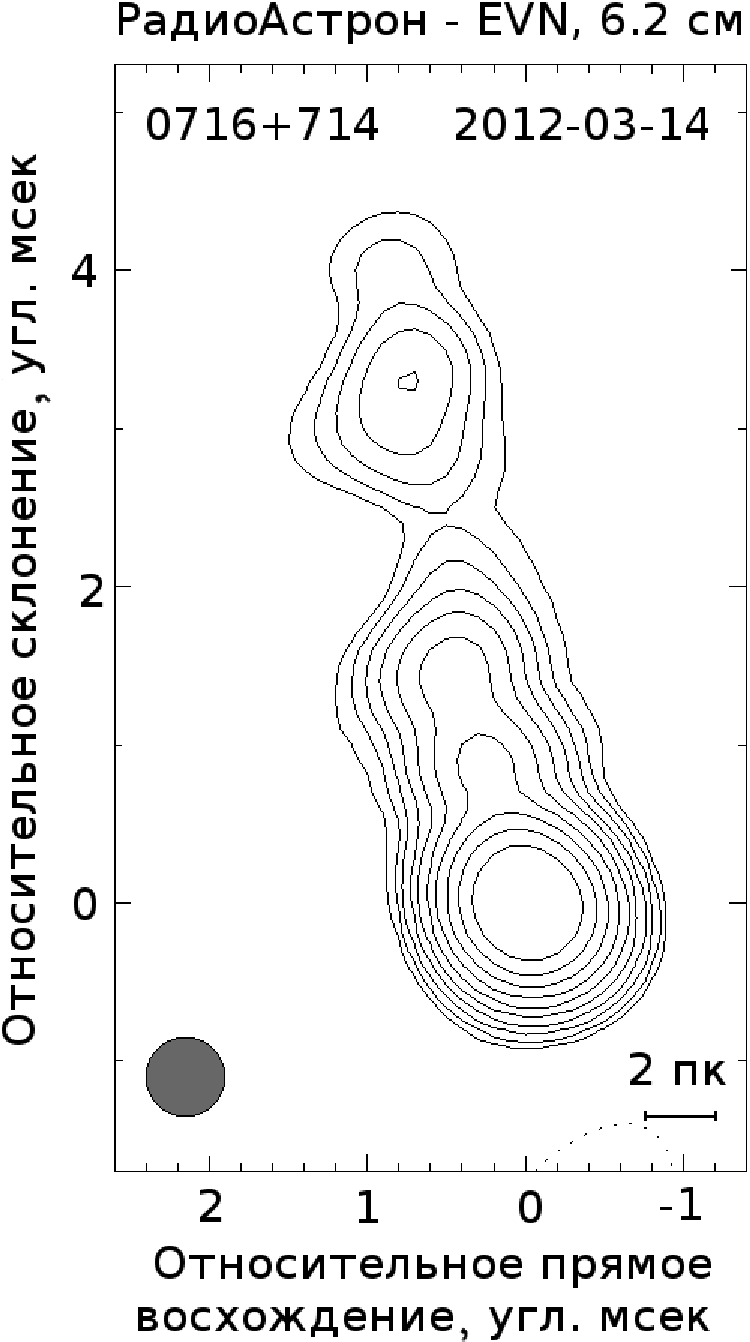
\includegraphics[scale=0.5]{map_0716+714.pdf}
 }
 \caption{Изображение быстропеременного объекта типа BL Lacertae 0716+714, полученное
по данным на длине волны 6.2 см. Наблюдения проведены совместно КРТ и Европейской
РСДБ-сетью 14--15 марта 2012 г. в рамках Ранней научной программы проекта
<<РадиоАстрон>> по активным ядрам галактик. Карта восстановлена
с использованием диаграммы направленности шириной 0.5 мсек. дуги
по уровню половинной мощности, сечение которой показано в левом нижнем углу
рисунка.  Контуры проведены по уровню равной интенсивности с
возрастанием в два раза для каждого следующего уровня, начиная с 0.25 мЯн/луч.
Интенсивность в максимуме равна 0.43 Ян/луч. <<Луч>> (<<beam>>) есть телесный
угол показанного сечения.}
 \label{fig:map_0716}
\end{figure}


\section{Измерение и анализ основных параметров космического телескопа <<РадиоАстрон>> в полете в
2011--2013 гг.}

\subsection{Введение}

Описание КА Спектр-Р, космического радиотелескопа (КРТ), научной аппаратуры и наземных испытаний
даны в \cite{Khartov_2011,Alexandrov_2011a,Alexandrov_2011b}. Результаты летных испытаний, методика
и первые результаты антенных измерений основных параметров телескопа радиоастрономическими методами
в радиометричесом режиме для диапазонов 92, 18, 6.2 и 1.35 см приведены в
\cite{Avdeev_2012,Kardashev_2013_rus,RAUH} --- для эффективной площади, шумовой температуры,
диаграммы направленности, погрешности наведения на источник и др.

В данной статье сообщается о новых результатах периодического контроля основных
антеных параметров, полученных в течение 2011--2013 гг. Измерения выполнены  как
в специальных сеансах наблюдений известных общепринятых первичных калибровочных
астрономических объектов, так и в процессе текущих сеансов массовых научных
наблюдений в режиме наземно-космического радиоинтерферометра со сверхбольшой
базой (РСДБ) --- как часть данных, требующихся для калибровки РСДБ наблюдений по
спектральной плотности потока излучения при выполнении Ранней научной программы
исследований.

Впервые представлены результаты антенных измерений в 8 поддиапазонах интервала частот 18--25 ГГц,
предназначенных для их использования в режиме многочастотного синтеза изображений в дальнейших
работах с РСДБ. Для калибровки этих измерений по потоку, кроме известных протяженных первичных
калибровочных источников (Кассиопея А, Лебедь А, Краб, Дева А), использовались также несколько
квазиточечных для КРТ сильных переменных внегалактических объектов (3С 84, 3С 273, 3C 279),
спектральные плотности потока излучения которых в близкие даты измерялись по известным вторичным
калибраторам на радиотелескопе РАТАН-600 Специальной астрофизической обсерватории РАН (Нижний Архыз,
Россия) и 100-м телескопе Института радиоастрономии общества Макса Планка (Эффельсберг, Германия).

\subsection{Измерения}

Измерения антенных параметров основаны на относительных измерениях эквивалентной спектральной
плотности потока шумового излучения системы $F_{sys}$ [Ян] (SEFD) --- относительно астрономических
калибраторов. Эквивалентная шумовая температура системы (радиотелескопа) $T_{sys}$ измерялась
относительно считающейся известной антенной температуры бортовых генераторов шумового сигнала (в
градусах К), входящих в состав каждого научного приемника.

Бортовой научный комплекс включает в себя 4 радиоастрономических супергетеродинных приемника --- на
диапазоны 92, 18, 6.2 и 1.35 см. Приемник диапазона 1.35 см обеспечивает также прием сигнала в 8
переключаемых поддиапазонах от 1.7 до 1.2 см с помощью выбора одного из поддиапазонов
соответствующими командами. Блоки входных малошумящих усилителей (МШУ) приемников всех диапазонов,
кроме 92 см, вынесены в открытый космос и размещены на <<холодной плите>>, охлаждаемой до
температуры 130 К радиационным способом. Каждый приемник состоит из 2-х идентичных каналов, на входы
которых от антенны через блок антенных облучателей (БАО) с разделителями поляризаций поступает
излучение в левой и правой круговых поляризациях. Каждый канал имеет два параллельных выхода: 1)
радиометрический выход --- с продетектированным сигналом, который поступает на телеметрическую
систему космического аппарата и используется в антенных измерениях, 2) интерферометрический выход
--- с сигналом на промежуточной частоте, который после дальнейших преобразований используется в
работе наземно-космического интерферометра.

Специальные сеансы наблюдений калибровочных объектов обычно проводились в режиме работы одиночного
телескопа. Тогда телеметрическая информация после буферной записи и хранения в бортовом
запоминающеем устройстве передавалась на Землю в течение суток через малонаправленную антенну по
служебному телеметрическому радиоканалу космического аппарата. При интерферометрических наблюдениях
исследуемых источников данные телеметрической системы последовательно размещаются в заголовках
каждого кадра потока данных для интерферометра и передаются на Землю в реальном времени через
остронаправленную антенну диаметром 1.5 м по научному высокоинформативному радиоканалу. Это дает
возможность выделять телеметрируемый радиометрический сигнал из интерферометрического потока данных
с КРТ. Таким путем в данной работе получены результаты антенных измерений по источникам, исследуемым
с интерферометром в научных программах.


\subsection{Обсуждение измерений}
\subsubsection{Диапазоны 92, 18, 6.2 и 1.35 см}

Анализ измерений показывает, что практически все основные антенные параметры иcпытывают вариации от
измерения к измерению, основную причину которых мы связывем с изменениями температурных условий
(соответствующих проектным), в которых находятся антенно-фидерный тракт и приемники. Физические
температуры элементов антенно-фидерного тракта и входных блоков МШУ приемников могут меняться из-за
изменений угла между направлениями на Солнце и объект измерения от сеанса к сеансу. Чем ближе этот
угол к проектной границе ($\approx 110^\circ$) допустимой работы КРТ, тем больших отклонений от
средних значений можно ожидать. При этом должен меняться и вклад в эквивалентную температуру системы
от потерь в антенных облучателях с разделителями поляриризаций, поэтому можно ожидать также заметных
вариаций эффективной температуры $T_{NS}$ калибровочного сигнала. Этот сигнал от внутреннего
шумового генератора поступает в тракт приемника на входе блока МШУ и приводится ко входу системы
телескопа, <<пересчитываясь>> через все элементы антенно-фидерного тракта.

Поэтому ниже для упрощения анализа предполагалось выполненным условие постоянства средних значений
$T_{NS}$ и  эффективной площади $A_{eff}$. Тогда все их реальные вариации автоматически относятся на
счет изменений $T_{sys}$. Заметим, что такая процедура не влияет на корректность <<астрономической
калибровки>> измерений с помощью параметра $F_{sys}$ (SEFD), зависящего от отношения $T_{sys} /
A_{eff}$. Обоснованием допустимости этого условия в данном случае могут служить приведенные ниже
результаты для среднеквадратичных отклонений $T_{sys}$ и $F_{sys}$ по калибровочным и исследуемым
источникам, которые не превышают примерно 13\%.

В пределах погрешности измерений полученные результаты для средних значений системной температуры
$T_{sys}$ и плотности потока $F_{sys}$ (SEFD) в диапазонах 92, 18, 6.2 и 1.35 см, с учетом
различного вклада вклада фона неба, согласуются как для калибровочных и исследуемых источников, так
и с первыми результатами, приведенными в работе \cite{Kardashev_2013_rus}: в пределах (20--25)\%
для диапазона 1.35 см и (10--15)\% для остальных диапазонов. Вместе с тем нельзя исключить, что
около половины от этих значений связана с медленной систематической эволюцией данных параметров,
включая их калибровку.

Заметный вклад в наблюдаемое рассеяние значений $T_{sys}$ относительно среднего может давать
изменение рассогласования МШУ с трактом <<БАО-вход МШУ>> и связанное с этим изменение коэффициента
шума МШУ, которые зависят от физических температур БАО и МШУ (развязки на входе МШУ, как обычно,
отсутствуют для понижения шумовой температуры приемника).

\subsubsection{Диапазон (18--25) ГГц}

Диапазон предназначен для использования в режиме многочастотного синтеза интерферометра и состоит из
8 следующих поддиапазонов (с указанными центральными частотами), отстоящих друг от друга на 960 МГц
\cite{Kardashev_2013_rus}: $F_{-4}$ (18392 МГц), $F_{-3}$ (19352 МГц), $F_{-2}$ (20312 МГц),
$F_{-1}$ (21272 МГц), $F_0$ (22232 МГц), $F_1$ (23192 МГц),  $F_2$ (24152 МГц), $F_3$ (25112 МГц)
--- см. рис. 3. Значения центральных частот могут быть на 4 МГц больше или меньше указанных, в
зависимости от заданного режима работы научной аппаратуры. Результаты измерений $F_{sys}$
($SEFD_{SRT}$) в этих поддиапазонах, приведенные на Рис.~3, и оценка чувствительности интерферометра
в Табл.~3 подтверждают теоретически ожидаемый монотонный <<ход>> $SEFD_{SRT}$ и чувствительности
интерферометра с ростом частоты, за исключением, быть может, их поведения на крайних частотах --
около 18 и 25 ГГц. Приведенные в табл.~3 чувствительности  рассчитаны по известной формуле
\cite{Kardashev_2013_rus}
$$
\sigma_{GBT-SRT} = b\, \sqrt{\frac {SEFD_{GBT}\, SEFD_{SRT}}{2\, \Delta \nu_{IF} \Delta t}},
$$
\noindent
где $b = 1/0.637$, $SEFD_{GBT} = 23$ Ян (для радиотелескопа НРАО в Грин Бэнке),
$\Delta \nu_{IF} = 16$~МГц --- полоса регистрируемых частот, $\Delta t = 5$~мин ---
время интегрирования сигнала. В зависимости от режима
работы интерферометра возможна также регистрация сигнала в полосе $\Delta\nu_{IF} = \SI{32}{\MHz}$
\cite{Kardashev_2013_rus}. Значение $\Delta\nu_{IF} = \SI{16}{\MHz}$ использовано для единообразия с
\cite{RAUH}.

Из данных на рис. 3 и в табл. 3 следует возможность проведения интерферометрических измерений в этом
режиме в пяти длинноволновых поддиапазонах c $F_{-4}$ по $F_0$ c чувствительностью не ниже, чем в
$F_0$ на частоте 22 ГГц (длина волны 1.35 см). В трех коротковолновых поддиапазонах $F_1$, $F_2$ и
$F_3$ оцененная чувствительность может быть до полутора раз меньше, чем в $F_0$, из-за более
сильного вклада фазовых погрешностей на длинах волн меньше 1.35 см. Эта длина волны близка к так
называемой <<проектной минимальной длине волны использования телескопа>> $\lambda_{min} \equiv
(16\text{--}20)\sigma \approx 18\sigma= \SI{1.39}{\cm}$ при проектном значении $\sigma =
\SI{0.77}{\mm}$ (подробнее см. \cite{Esepkina_1973,Kuhn_1967,Cejtlin_1976} и разделы 3.2 и 3.3
ниже).

\begin{table}
\caption{Результаты массовых измерений и расчетных оценок при наблюдениях калибровочных и
исследуемых источников в левой (LCP) и правой (RCP) круговых поляризациях в 2011--2013 гг.
\tiny{Примечание. Измерения калибраторов в диапазонах 1.35 и 6.2 см даны за 2011–2012 гг. Ошибки
шкалы спектральной плотности потока не включены. В строках 3.3–3.6 и 3.7 (3.10) даны оценки вкладов
в $T_{sys}$ от шумовых температур приемника $T_{rec}$, кабеля (волновода – в диапазоне 1.35 см)
$T_{Cable}$, блока антенных облучателей $T_{BAO}$, антенны $T_a$ и фона неба $T_{sky}$,
соответственно.
}}
\bigskip
\label{tab:srt_params2}
\centering
    \begin{SingleSpace}
    \tiny
        \begin{tabular}{lcccc}
        \toprule
Параметр              & 1.35 см  & 6.2 см   & 18 cм    & 92 см\\
                      & LCP; RCP & LCP; RCP & LCP; RCP & LCP; RCP\\

        \midrule
1 КАЛИБРАТОРЫ              & & & &\\
1.1 $T_{sys}$, K    & $98\pm13$; $82\pm11$    & $133\pm17$; --  &
$47.2\pm1.0$ ; $48.4\pm1.0$  & $230\pm5$; $210\pm11$ \\
1.2 $F_{sys}$, кЯн  & $36.0\pm3.6$; $30\pm3.0$ & $10.5\pm1.1$; -- & $3.18\pm0.06$; $3.26\pm0.07$
& $21.2\pm0.42$; $19.4\pm1.0$\\
2 ДРУГИЕ объекты         & & & &\\
2.1 $T_{sys}$, K    & $127\pm8$; $100\pm10$      & $147\pm8$; --  & $41.0\pm1.0$; $43.5\pm4.0$
& $145\pm15$; $147\pm15$\\
2.2 $F_{sys}$, кЯн  & $46.7\pm3.0$; $36.8\pm3.7$ & $11.6\pm0.63$; -- & $2.76\pm0.27$; $2.93\pm0.27$
& $13.3\pm1.4$; $13.5\pm1.4$\\
\midrule
3 РАСЧЕТ $T_{sys}$ и $F_{sys}$.& & & &\\
3.1 Коэффиц. передачи: & & & &\\
--- Kабеля $K_3/t_3$  &  0.99/157      & 0.94/157        & 0.95/157       & 0.98/233 \\
--- БАО $K_2/t_2$     &  0.76;0.84/175 & 0.68/175        & 0.95/175       & 0.83/175 \\
--- Aнтенны $K_1/t_1$ &  0.98/200      & 0.98/200        & 0.98/200       & 0.98/200 \\
3.2 $T_{rec} / t_4$, K   & 45 /140 & 26/140 & 15/140 & 39/290\\
3.3 $\Delta T_{rec}$, K  & 61; 55     & 42     & 17     & 49    \\
3.4 $\Delta T_{Cable}$, K&  2         & 15     & 8.9    &  6    \\
3.5 $\Delta T_{BAO}$, K  & 56; 34     & 84     & 9.4    & 36    \\
3.6 $\Delta T_A$, K      & 4          &  4     & 4      &  4    \\
3.7 $T_{sky}$, K         & 3          &  3     & 3      &  3+50 \\
3.8 $T_{sys}$, K         & 126; 98    & 148    & 42.3   &  98+50\\
3.9 $F_{sys}$, кЯн     & 46.4; 36.1& 11.7& 2.85   & 13.6  \\
Калибраторы: & & & & \\
3.10 $T_{sky}$, K         &    --       &  --     & $3+5$    &  $3+120$  \\
3.11 $T_{sys}$, К         &    --       &  --     & $42.3+5$ &  $98+120$ \\
3.12 $F_{sys}$, кЯн       &    --       &  --     & $3.18$   &  $19.5$    \\
        \bottomrule
        \end{tabular}
    \end{SingleSpace}
\end{table}

\begin{table}
\caption{Основные параметры КРТ по \cite{Kardashev_2013_rus} и новым измерениям.
\tiny{Примечание. В строках 1--11 даны: ширина главного лепестка диаграммы направленности по уровню
половинной мощности --- 1, эффективная площадь --- 2, коэффициент использования площади --- 3,
эквивалентная температура шума и плотность потока шумового излучения системы --- 4 и 5, усиление
телескопа --- 6, систематическая погрешность при сканировании площадки неба
по двум координатам (строки 7 и 8) после ввода постоянной поправки (строка 9) в наведение телескопа,
чувствительность интерферометра КРТ – Green Bank Telescope по (1) и [6] --- 10, отношение
измеренной ширины к идеальной ширине $\lambda/\text{D}$ главного лепестка диаграммы направленности
--- 11.}}
\bigskip
\label{tab:srt_params3}
\centering
    \begin{SingleSpace}
    \tiny
        \begin{tabular}{lcccc}
        \toprule
Параметр              & 1.35 см  & 6.2 см   & 18 cм    & 92 см\\
                      & LCP; RCP & LCP; RCP & LCP; RCP & LCP; RCP\\

        \midrule
КРТ в полете, 2011--2013: & & & &\\
                       & & & &\\
1. $(\vartheta_{0.5} \pm 5 \%) \times (\varphi_{0.5} \pm 5 \%)$ & $6.0' \times 13'$ & $25'$ &$72'$
 & $6^\circ.1$ \\
2. $A_{eff} \pm 10\%$, м$^2$                  & 7.5        & 35     & 41         & 30\\
3. КИП = $A_{eff}/A_{geom} \pm 10\%$          & 0.1        & 0.45   & 0.52       & 0.38\\
4. $T_{sys} \pm 10\%$, K                      & 127; 100   & 147;  -- & 41.0; 43.5 & 145; 147\\
5. $F_{sys} \pm 10\%$ (SEFD), кЯн             & 46.7; 36.8 & 11.6; --& 2.76; 2.93 & 13.3;13.5\\
5. Усиление, Ян/K                             & 368        &  78.9  & 67.3       & 92.0     \\
6. $\Delta \vartheta_s$  & $-1.2' \pm 0.2'$    & & & \\
7. $\Delta \varphi_s$    & $< 1.5'$            & & & \\
8. $\delta \varphi_p$    & $2.5'$              & & & \\
9. $\sigma_{SVLBI}$, мЯн          & 17; 15 &  5; --  & 3; 3    & 14; 14\\
   (при $\Delta t = 5$ мин; $\Delta \nu = 16$ Мгц)            &        &        &         &
\\
10. $\alpha_D = (\vartheta_{0.5} \times \varphi_{0.5}) \cdot D / \lambda$ &  1.29 x 2.80 & 1.17 &
1.16 & 1.16\\
        \bottomrule
        \end{tabular}
    \end{SingleSpace}
\end{table}

\subsection{Заключение}

Новые результаты радиометрических измерений параметров космического радиотелескопа в 2011–2013 годах
по калибровочным объектам с помощью одиночного КРТ и по большому количеству исследуемых источников в
режиме интерферометра согласуются с первыми результатами, полученными Кардашевым и др. [5], --- в
пределах (10--15)\% в диапазонах 92, 18 и 6.2 см и (20--25)\% в диапазоне 1.35 см.

Основной вклад в SEFD и чувствительность КРТ в диапазонах 92, 18 и 6.2 см вносят шумы приемника и
блока антенных облучателей, а в диапазоне 1.35 см – потери эффективной площади из-за фазовых
погрешностей в антенно-фидерной системе. Вклад КРТ в чувствительность наземно-космического
интерферометра, пропорциональный корню квадратному из измеренных значений SEFD, близок к проектному
в диапазонах 92 и 18 см и уменьшает проектную чувствительность примерно в 1.5 и 2 раза в диапазонах
6.2 и 1.35 см, соответственно. Измеренный вклад КРТ увеличивает чувствительность интерферометра до
1.5 раз в 5-ти поддиапазонах на частотах от 22 до 18 ГГц и уменьшает ее до 1.5 раз в 3-х
поддиапазонах на частотах от 22 до 25 ГГц относительно чувствительности на 22 ГГц.

Основной вклад в эквивалентную шумовую температуру КРТ вносят приемник и блок антенных облучателей
(БАО) с разделителями поляризаций. Разброс значений этой шумовой температуры, через зависимость от
физических температур МШУ и БАО, может быть связан с изменениями ориентации КРТ относительно Солнца
в индивидуальных сеансах наблюдений.

Полученные результаты и опыт эксплуатации КРТ могут быть полезны при разработке будущих космических
проектов (<<Миллиметрон>> и др.; особенно учитывая, что антенна КРТ, вероятно, самая большая на
сегодня конструкция, раскрытая в космосе). Они указывают на необходимость проектной оптимизации
фазовых погрешностей поверхности и облучения зеркала и минимизации потерь как в отдельных элементах,
так и в антенно-фидерной системе с приемниками в целом. Для уменьшения фазовых искажений вблизи
минимальной длины волны использования телескопа может оказаться целесообразным дополнительное
проектное недооблучение края зеркала, уменьшающее известный оптимальный уровень в несколько раз.


\section{RadioAstron space VLBI imaging of polarized radio emission in the high-redshift quasar
0642+449 at 1.6 GHz}

\subsection{Подгонка лепестков}

Подгонка интерференционных лепестков проходила в два этапа: сначала применялась ручная коррекция
фазы, а затем использовался глобальный поиск лепестков для определения частоты интерференции на
антеннах и одно и многополосные задержки. Также была исправлена разность групповых задержек между
каналами поляризации. Полученные значения частоты интерференции для наземно-космических баз
представлены на рис.~\ref{fig:0642_rate}. Эта плавно меняющаяся остаточная частота
хорошо согласуется с ожидаемой точность определения орбитальной скорости КРТ
\cite{Kardashev_2013_rus}, но всё же она должна
рассматриваться только как индикатор качества данных, в то время как более подробное обсуждение
точности восстановления орбиты КРТ представлено в работе \cite{Duev_2015}.

\begin{figure}[]
 \centerfloat{
  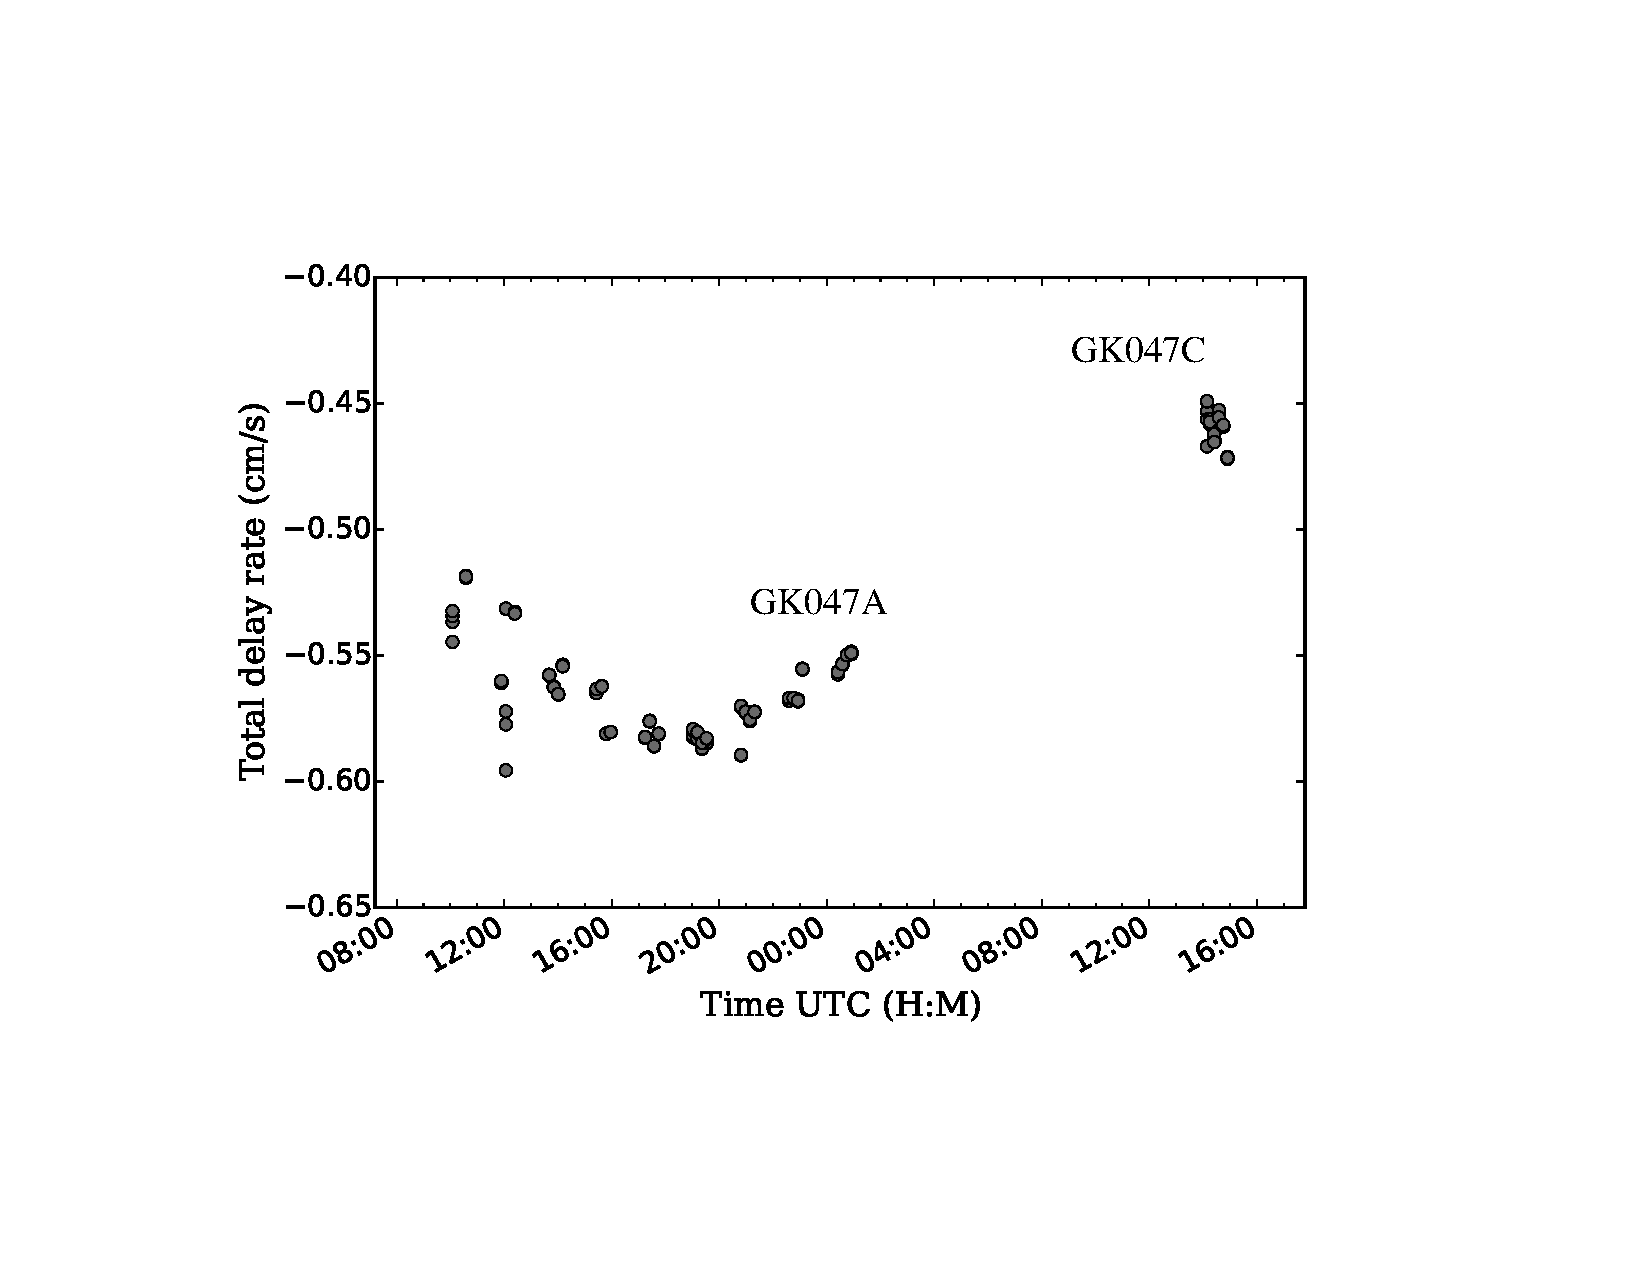
\includegraphics[width=0.9\textwidth]{totalrate.pdf}
 }
 \caption{Полная частота интерференции, полученная из подгонки лепестков на базе КРТ-Эффельсберг и
включающая в себя изменение хода часов каждого из телескопов. Для каждого наблюдательного сегмента
КРТ была получена частота интерференции с помощью подгонки лепестков на временном интервале 10
минут. Частоты нарисованы отдельно для каждого частотного и поляризационного канала. Рисунок
отражает точность определения скорости при реконструкции орбиты КРТ. Все значения скорости и
ускорения являются проекциями истинный остаточных скорости и ускорения космического аппарата.}
 \label{fig:0642_rate}
\end{figure}


\section{RadioAstron orbit determination and evaluation of its results using correlation of
space-VLBI observations}

\subsection{Введение}

Космический аппарат РадиоАстрон, оснащенный 10-метровым космическим радиотелескопом (КРТ), был
запущен на высокоэллиптическую орбиту Земли в июле 2011 года с помощью ракеты <<Зенит-3Ф>> с
разгонным блоком <<Фрегат-СБ>>. Основное назначение космического аппарата --- проводить наблюдения
галактических и внегалактических радиоисточников вместе с наземными радиотелескопами, образуя
многоантенный наземный радиоинтерферометр с чрезвычайно длинными базами \cite{Kardashev_2013_rus}.
Космический аппарат также позволил проверить Принцип эквивалентности Эйнштейна благодаря его
эксцентричной орбите и высокостабильному бортовому водородному стандарту частоты
\cite{Litvinov_2018,Nunes_2020}.

КРТ наблюдает в четырех частотных диапазонах: P, L, C и K. Во время наблюдений космический аппарат
передает полученные научные данные в реальном времени на станцию слежения на Земле, используя
1.5-метровую остронаправленную антенну через нисходящий канал 15 ГГц. Научная полезная нагрузка КРТ
включает в себя два водородных стандарта частоты (H-мазеры), причем в каждый момент времени работать
может только один из двух. Вскоре после запуска один из двух Н-мазеров был идентифицирован как
поврежденный, а другой полностью функционировал. Последний H-мазер, таким образом, использовался с
начала миссии в 2011 году по август 2017 года, когда он исчерпал запас водорода и был отключен, тем
самым превысив его ожидаемый срок службы в два раза. Научные приборы на КРТ и радиолиния передачи
данных может быть синхронизирована либо с бортовым сигналом H-мазера, либо с наземным сигналом
H-мазера, передаваемым от одной из станций слежения миссии RadioAstron. Пока работал бортовой
H-мазер, его сигнал, как немного более стабильный, чем сигнал восходящей линии связи, использовался
в качестве эталона как для научной аппаратуры, так и для сигналов нисходящей линии связи, включая
анализируемые в этой статье.

Радиолиния С-диапазона используется для телеметрии и управления, а также для получения данных о
дальности и доплеровском слежении для нужд определения орбиты. Регулярное отслеживание выполняется
каждые 2--3 дня с помощью двух антенн, расположенных в России: 64-метровой антенны в Медвежьих
озерах (под Москвой) и 70-метровой антенны в Уссурийске (Приморский край). РадиоАстрон также оснащен
уголковым отражателем, который позволяет проводить лазерные измерения дальности.

Орбита РадиоАстрона высоко эллиптическая, геоцентрическое расстояние варьируется от 7000 до
351\,600~км, а средний период составляет 8.6 дня. Орбита космического аппарата значительно
эволюционирует со временем из-за гравитационного воздействия третьих тел. Параметры орбиты
периодически изменяются с периодом около 2 лет, что дает широкие возможности наблюдения различных
радиоисточников, распределенных по всему небу.

Обработка РСДБ данных включает в себя так называемую процедуру поиска интерференционных лепестков,
то есть поиск максимума взаимной корреляции сигналов, записанных на разных телескопах. Эта
процедура требует, чтобы задержка времени прихода волнового фронта на каждой паре телескопов была
точно известна на время наблюдения. Начальное предположение для задержки рассчитывается в
соответствии с моделью, которая использует различные виды данных: траектории фазовых центров
участвующих телескопов в инерциальной системе отсчета, поправки и дрейф часов, параметры среды
распространения и т.д. Чтобы выполнить поиск лепестков за разумное время, скажем десятки минут,
используя современный вычислительный кластер, априорная неопределенность в параметрах модели должна
быть относительно небольшой и известной (требуемый уровень неопределенности зависит от многих
факторов, несколько примеров приведены ниже).

В космическом РСДБ основная неопределенность в моделируемой задержке и ее производных связана с
ошибками реконструкции орбиты космического аппарата, несущего радиотелескоп. Для
космического аппарата миссии РадиоАстрон перед запуском были установлены следующие требования к
точности определения орбиты:

\begin{itemize}
 \item ошибка положения меньше \SI{600}{\meter};
 \item ошибка скорости меньше \SI{2}{\cm\per\second};
 \item ошибка ускорения меньше \SI{e-8}{\meter\per\square\second}
\end{itemize}

Эти требования определяются несколькими факторами, в том числе: длина волны наблюдения,
скорость передачи данных, количество участвующих телескопов, конструкция коррелятора, доступные
вычислительные ресурсы и т.д.

Требование к точности положения формально отражает окно поиска по задержке шириной 128
спектральных каналов. Фактический размер окна и количество каналов, используемых коррелятором,
значительно больше, например, 2048 спектральных каналов для обзора активных ядер галактик (AGN), что
позволяет учесть разные виды ошибок. Ошибка скорости менее \SI{2}{\cm\per\second} позволяет
выполнять поиск лепестков на самой короткой длине волны (\SI{1.35}{\cm}), используя время
интегрирования в корреляторе всего 1/8~с. Довольно жесткие требования к точности ускорения
изначально возникли из-за необходимости ограничения фазовых ошибок в K-диапазоне на
интервале интегрирования $\sim$10 минут в пределах одного радиана. Однако ошибка ускорения в
пределах окна \SI{+-1.5e-6}{\meter\per\square\second} может быть компенсирована коррелятором во
время обработки.

Для более ранней и пока единственной реализованной космической РСДБ-миссии VSOP/HALCA требования
к определению орбиты были аналогичными (дана ошибка в $1\sigma$): положение --- \SI{80}{\meter},
скорость --- \SI{0.43}{\cm\per\second}, ускорение --- \SI{6e-8}{\meter\per\square\second}
\cite{You_1998}. Сходство легко понять, поскольку VSOP/HALCA был спроектирован для наблюдения на
сопоставимых длинах волн 1.35, 6 и 18 см и записывал данные с той же скоростью передачи данных, что
и РадиоАстрон (\SI{128}{\mega\bit\per\second}). Несмотря на то, что научные наблюдения с
использованием HALCA обычно проводились только на частотах 1.6 и 5 ГГц из-за проблем
чувствительности на частоте 22 ГГц, требования к определения орбиты были сформулированы для всех
трех полос. Чуть более строгие требования VSOP к точности определения местоположения и скорости
связаны с другой конструкцией коррелятора.

Определение орбиты космического аппарата РадиоАстрон осложняется ограниченной поддержкой слежения и
значительными негравитационными возмущениями, вызванными давлением солнечной радиации (SRP) и
автономными включениями двигателей системы управления ориентацией космического аппарата. Уникальной
особенностью космического аппарата, выполняющего РСДБ наблюдения, является возможность проверки
точности определения его орбиты с использованием так называемых остаточных задержек и частот
задержки, полученных в результате успешного детектирования интерференционных лепестков и
посткорреляционного анализа. В этой работе мы суммируем первый опыт оценки точности определения
орбиты, основанный на использовании остаточных величин, полученных при наблюдениях космического
РСДБ. В отличие от данных наблюдений на линии прямой видимости, этот вид данных позволяет измерять
погрешности положения и скорости космического аппарата, проецируемых на разные направления. Этот
анализ позволил нам количественно оценить точность двух версий алгоритма определения орбиты.

\subsection{Описание коррелятора АКЦ}

Орбитальные решения, полученные в результате процедуры OD, описанной выше, используются главным
образом для научных приложений, прежде всего для корреляции РСДБ данных, собранных миссией.
В этом разделе мы рассмотрим работу одного из корреляторов, способных обрабатывать данные
РадиоАстрон, а именно коррелятора АКЦ. Этот FX-коррелятор был разработан в Астрокосмическом центре
Физического института им.~П.Н.~Лебедева (АКЦ ФИАН) специально для поддержки миссии РадиоАстрон
\cite{Likhachev_2017}. Он использовался для обработки большинства наблюдений, выполненных на
РадиоАстроне, и, таким образом, предоставляет самый большой набор данных о так называемых остаточных
задержках и частотах интерференции, который мы будем использовать в следующем разделе для оценки
точности определения орбиты.

Корреляция данных космического РСДБ выполняется Коррелятором АКЦ в два этапа, причем второй этап
необходим из-за неопределенности определения орбиты. Чтобы уменьшить остаточную задержку, частоту
задержки и ускорение задержки, первый шаг, или проход, выполняется в так называемом режиме
<<широкого>> окна. Размер окна по задержке определяется числом спектральных каналов, а по частоте
интерференции~"--- временем интегрирования. Оба параметра устанавливаются до начала процесса
корреляции и могут быть легко отрегулированы. После того как найден интерференционный лепесток,
второй проход корреляции выполняется в меньшем окне с учетом остаточных задержек, полученных в
первом проходе.

Способность РадиоАстрона одновременно наблюдать на двух разных длинах волн имеет большое значение
для поиска лепестков. В случае, когда наблюдение проводилось на двух разных длинах волн, остаточные
значения, полученные в результате успешного поиска лепестков на большей длине волны, могут
использоваться для значительного упрощения поиска лепестков на более короткой.

Модель задержки для космического РСДБ естественно более сложна, чем та, которая используются для
наземного РСДБ. Помимо вопросов, связанных с орбитой, необходимо учитывать тот факт, что частота
задержки зависит не только от относительных скоростей телескопов, но и от сдвига частоты сигнала
восходящей линии связи, которая используется на борту в качестве эталона для бортового научного
оборудования (для режима синхронизации замкнутой петлей) или смещение частоты
бортового H-мазера (для однопутевого режима). В последнем случае, поправка к частоте интерференции
может достигать величины \SIrange{30}{35}{\pico\second\per\second}.

Отличительной особенностью коррелятора АКЦ является его модель задержки ORBITA2012. Эта модель
задержки была разработана специально для коррелятора ASC и способна рассчитывать задержку до членов
$O(c^{-3})$ \cite{Vlasov_2012}, что предусматривает использование меньших размеров окна корреляции
на первом проходе процесса корреляции. Более того, эта модель задержки способна учитывать ускорение
задержки.

Посткорреляционная обработка данных всех экспериментов, рассмотренных в этой статье, была
выполнена в пакете PIMA \cite{Petrov_2011}. Она включала в себя подгонку интерференционных
лепестков, калибровку полосы пропускания и амплитуды, а также усреднение данных по времени и
частоте. Основной целью посткорреляционной обработки является изучение физических свойств
наблюдаемых объектов. Остаточные значения групповой задержки, частоты задержки и ускорения задержки
являются побочным продуктом этой обработки. Полная задержка и ее производные могут быть
в дальнейшем использованы для изучения наблюдаемых объектов, например, при картографировании.
Это требует точной калибровки ряда неопределенностей, таких как, ход часов на телескопе, их
траектории (в том числе КРТ), координаты наблюдаемых источников, параметры среды распространения и
т.д.

Остаточные задержки и их производные, которые мы использовали в этом анализе, были получены в
результате корреляции наблюдений научной программы обзора АЯГ на РадиоАстроне и не использовались
в процедуре OD. Источники, наблюдаемые в этой программе, достаточно компактны, так что вклад в
остаточные значения из-за неточечной структуры источников незначителен.

\subsection{Результаты определения орбиты}

Алгоритм определения орбиты, описанный в этой статье, был реализован и использован Институтом
прикладной математики им.~М.В.~Келдыша (ИПМ) для предоставления пользователям РадиоАстрона
апостериорных орбит, необходимых для корреляции РСДБ данных, собранных миссией. Большинство
наблюдений, выполненных с 2014 года, и значительная часть предыдущих наблюдений были
скоррелированны с использованием орбит, полученных с помощью этой версии алгоритма. На ранних этапах
миссии, то есть для экспериментов, проведенных до 2014 года, использовалась предыдущая, менее
сложная версия алгоритма OD.

Статистически значимая корреляция, обнаруженная между сигналами, записанными космическим
радиотелескопом РадиоАстрон и наземными радиотелескопами, дает набор из трех остаточных значений:
задержки, частоты задержки и ускорения задержки. В этой статье мы фокусируемся исключительно на
значениях частоты задержки по следующим причинам. Во-первых, данные, собранные космическим
радиотелескопом, не имеют меток времени на борту, т.е. синхронизация шкалы времени H-мазера с UTC
возможна только косвенно, с помощью установки меток времени в потоке данных, поступающего со
спутника, на приемной станции слежения. Во-вторых, существует ненулевая вероятность несовместимой
синхронизации наземных радиотелескопов с UTC. И наконец, как показано ниже, существует ряд
существенных факторов, не связанных с орбитой, которые могут вносить вклад в частоту остаточной
задержки, также влияющую на остаточную задержку. Все это затрудняет отделение вклада в остаточную
задержку из-за ошибок на орбите от ошибок из-за задействованных часов. С другой стороны, возможные
вклады в частоту остаточных задержек гораздо более предсказуемы. Синхронизация времени с помощью
станции слежения не влияет на частоту задержки, так как любое изменение в задержке, которое она
может внести, остается постоянным в течение каждого <<скана>> (файла) записанных данных. Дрейф
наземных часов, как правило, намного меньше, чем частоты остаточных задержек, которые мы наблюдаем,
и, кроме того, когда в эксперименте задействовано более одного наземного радиотелескопа,
относительные дрейфы наземных часов можно оценить, выполнив поиск лепестков на наземных базах.
только базовые показатели. Наконец, дрейф часов на борту КРТ может быть оценен независимо в
процессе определения орбиты.

\begin{figure}
 \centerfloat{
    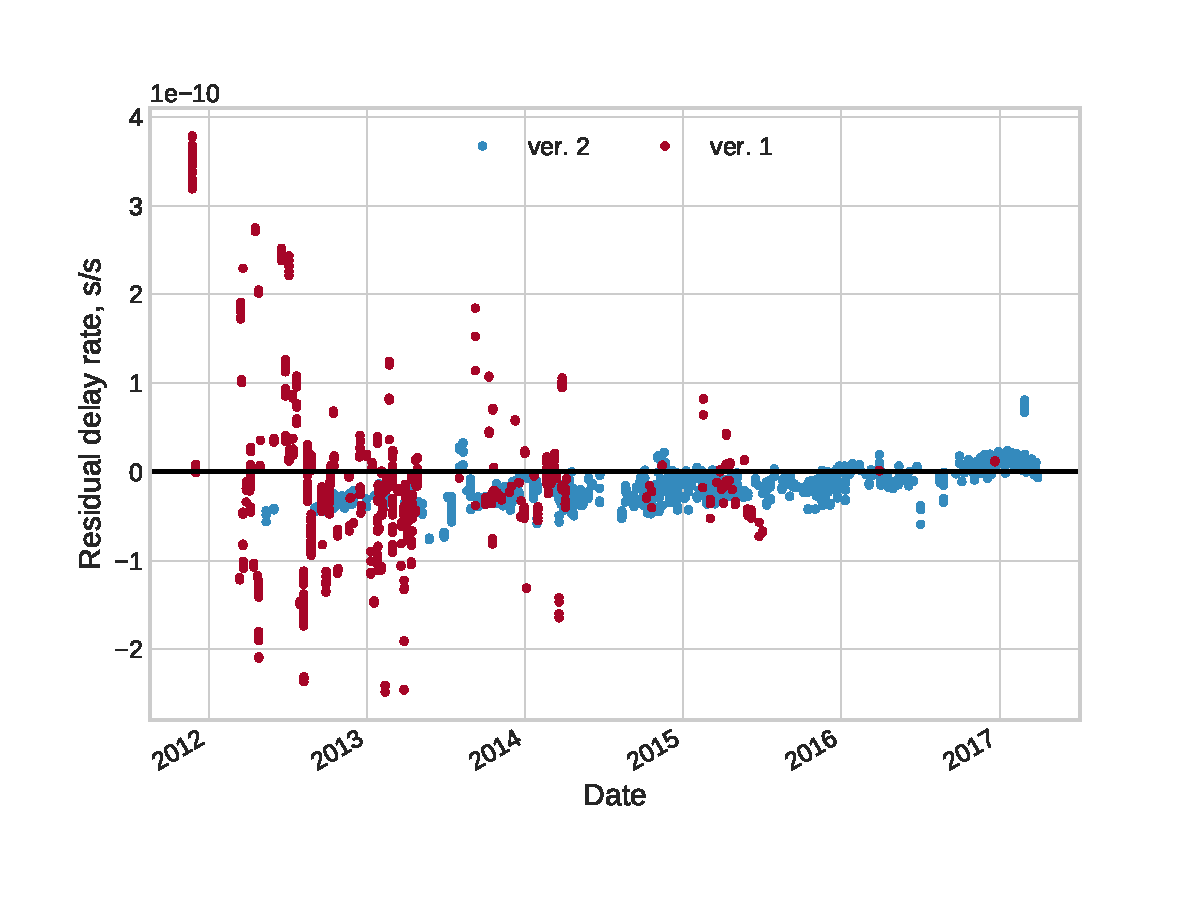
\includegraphics[width=0.7\textwidth]{raw_rrates_v1_v2.pdf}
 }
 \caption{Величины остаточной частоты задержки, полученные на корреляторе АКЦ с
использованием двух версий орбиты: универсальный алгоритм, версия 1 (красные точки); новый алгоритм,
версия 2 (синие точки). (Для интерпретации ссылок на цвет в этой легенде рисунка читатель обращается
к веб-версии этой статьи.)}
 \label{fig:rates_v1v2}
\end{figure}

На рис.~\ref{fig:rates_v1v2} показаны величины остаточной частоты задержки, полученные с помощью
коррелятора АКЦ в результате обработки наблюдений, выполненных миссией РадиоАстрон до начала 2017
года. Каждая точка данных на рис.~\ref{fig:rates_v1v2} соответствует значению остаточной частоты
задержки, определенной коррелятором. в результате корреляции двух сканов данных, то есть единиц
данных, обычно продолжительностью $\sim10$ минут, один из которых был записан космическим
радиотелескопом, а другой~"--- наземным радиотелескопом, который участвовал в эксперименте. Синие
точки обозначают остаточную частоту задержки, полученные с орбитами версии 2, т.е. те, которые
определены с помощью алгоритма, описанного в Разделе 4. Красные точки обозначают значения,
полученные на орбитах версии 1, т.е. определенные с помощью общего алгоритма OD и более простой
динамической модели космического аппарата. Более ранняя версия алгоритма использует простую модель
пушечного ядра для оценки SRP и, таким образом, игнорирует ее зависимость от ориентации. Кроме того,
изменения скорости из-за разгрузок не оцениваются в общем алгоритме, а устанавливаются на их
априорные значения. Для каждой точки на рис.~\ref{fig:rates_v1v2} предполагается, что КРТ является
первой антенной, а наземный радиотелескоп~"--- второй, то есть изображенные остаточные частоты
задержек являются относительными к космической антенне.

Все наблюдения, использованные для получения остаточных частот задержки на
рис.~\ref{fig:rates_v1v2}, проводились в так называемом однопутевом режиме, который
характеризуется следующими двумя условиями: (a) бортовое научное оборудование синхронизировано с
опорным сигнал бортового H-мазера; (b) несущая сигнала нисходящей линии связи, используемого для
передачи научных данных с космического аппарата на станцию слежения, также синхронизируется с
опорным сигналом H-мазера.

\begin{figure}
 \centerfloat{
    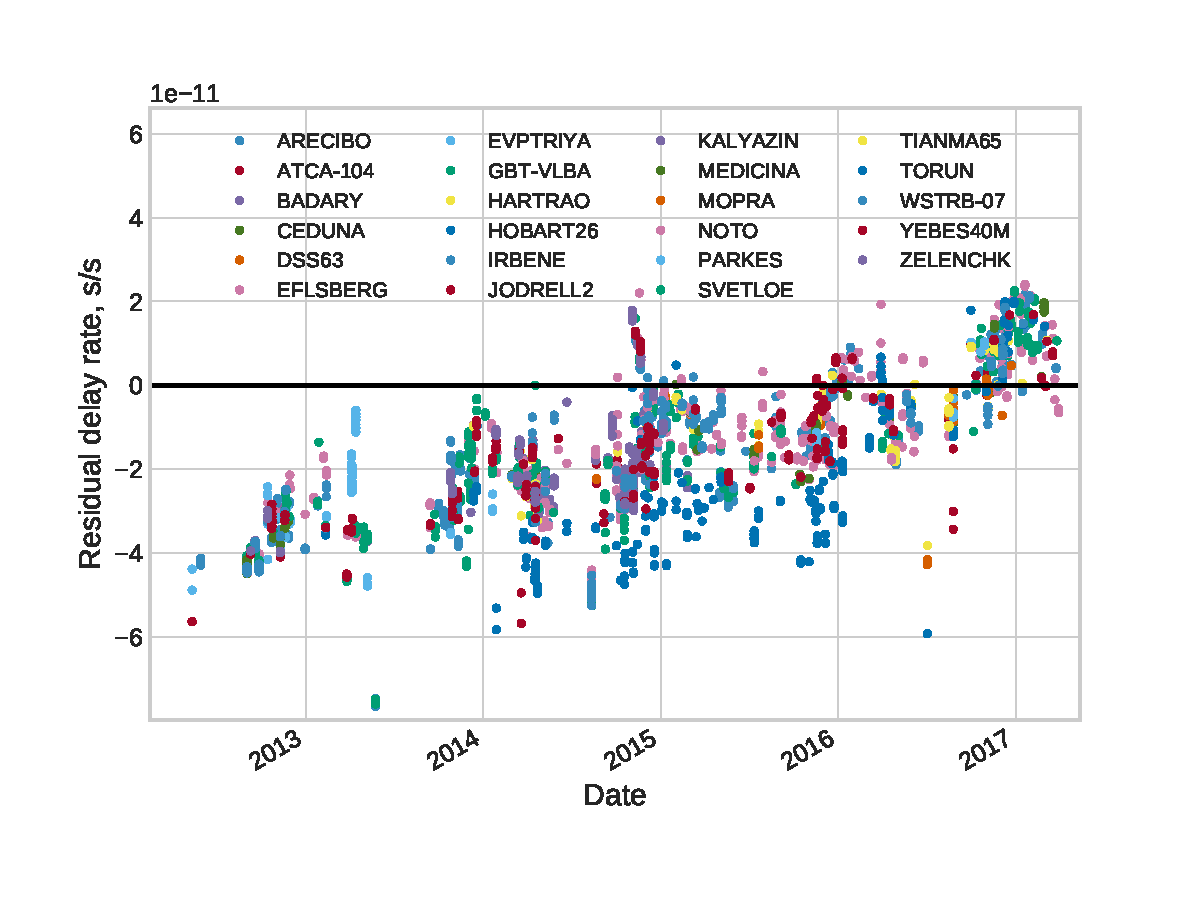
\includegraphics[width=0.7\textwidth]{raw_rrates.pdf}
 }
 \caption{Величины остаточной частоты задержки, полученные с использованием орбит версии 2. Цвет
указывает наземный радиотелескоп. (Для интерпретации ссылок на цвет в этой легенде
рисунка читатель обращается к веб-версии этой статьи.)}
 \label{fig:rrates}
\end{figure}

Из рисунка~\ref{fig:rates_v1v2} видно, что разброс остаточных частот задержки, полученных с
помощью версии 2 алгоритма OD, существенно меньше, чем у частот задержек, полученных с помощью
общего алгоритма. Среднеквадратическое значение остаточных частот задержек составляет
\num{2.463e-11} для версии 2 и \num{1.097e-10} для версии 1. Также ясно, что остаточные частоты
задержек, полученные на орбитах версии 2, смещены от нуля, а среднее значение равно
\num{1.663e-11}, а также показывают долгосрочный линейный тренд (рис.\ref{fig:rrates}). Последнее
явно указывает на систематический эффект, который нельзя отнести к ошибке OD, поскольку эти
остаточные значения были получены с использованием большого числа независимых решений и
еще большего числа наблюдений радиоисточников, рассеянных по всему небу и наблюдаемых на различных
проекциях баз.

\subsection{Выводы}

Мы изложили наш подход к определению орбиты космического аппарата РадиоАстрон. Этот метод включает
собственную модель давления солнечного излучения и алгоритм, позволяющий учесть накопленный момент
импульса маховиков для улучшения наших знаний о динамике центра масс космического аппарата.
Мы проверили эффективность этого метода определения орбиты, используя уникальные <<данные
слежения>>, доступные только для космического аппарата, участвующего в РСДБ наблюдениях, а именно
остаточные частоты задержек, которые в нашем случае были получены с помощью коррелятора АКЦ миссии
РадиоАстрон в результате обработки данных РСДБ-наблюдений небесных радиоисточников на КРТ совместно
с наземными радиотелескопами. Этот анализ позволил нам сделать вывод, что метод определения орбиты,
который мы разработали, обеспечивает до 11 раз более точные орбитальные решения с точки зрения
скорости и остаточных частот задержек по сравнению с обычным алгоритмом определения орбиты.
           % Глава 2
\graphicspath{{Dissertation/images/chapt3/}}

\chapter{Экстремальные яркостные температуры в обзоре активных ядер галактик} \label{chapt3}

\section{Яркостная температура}

\section{Обзор активных ядер галактик в проекте <<РадиоАстрон>>}


\section{RELATIVISTIC JETS IN THE RADIO REFERENCE FRAME IMAGE DATABASE. II. BLAZAR JET
ACCELERATIONS FROM THE FIRST 10 YEARS OF DATA (1994--2003)}
% \section{Измерение доплеровского усиления с помощью кинематики релятивистских струй}

\subsection{Введение}

Объемный отток вещества при высоких факторах Лоренца в коллимированных релятивистских струях
является хорошо известным свойством мощных блазаров. Такие высокие факторы Лоренца можно
непосредственно наблюдать по видимому движению высокоскоростных компонентов струи
на изображениях, построенных с помощью  интерферометрии со сверхдлинными базами (РСДБ)
\cite{Lister_2009b}, и они также необходимы для объяснения спектрального распределения энергии
блазаров \cite{Hartman_2001}, переменности гамма-излучения \cite{Dondi_1995} и высокой яркостной
температуры радио-ядра \cite{Tingay_2001}. Эти релятивистские джеты должны ускорятся на масштабах
расстояний от примерно $10^3$ гравитационных радиусов от центральной черной дыры и до парсеков, где
они непосредственно наблюдаются с помощью РСДБ \cite{Sikora_2005,Vlahakis_2004}. Хотя наблюдения за
потоками с высоким фактором Лоренца хорошо установлены, теоретический механизм, с помощью которого
эти потоки ускоряются, и масштаб длины, на котором они работают, до конца не поняты.

В общем контексте ускорения магнитной струи в блазарах \cite{Sikora_2005} энергия потока начинается
как магнитная энергия, или поток вектора Пойнтинга, который затем преобразуется в объемную
кинетическую энергию во время фазы ускорения и, наконец, в кинетическую энергию частиц при ударах,
которая затем может излучиться. Магнитное ускорение было исследовано с помощью релятивистского
магнитогидродинамического моделирования (например \cite{McKinney_2006}; также см.
\cite{Komissarov_2011,Konigl_2010} для краткого описания теории магнитного ускорения релятивистских
струй).

Остается рассмотреть ряд деталей в этой общей структуре: например, создается ли струя в устойчивом
состоянии или ускорение является импульсным \cite{Granot_2011,Lyutikov_2010}, и
завершается ли ускорение на масштабах, наблюдаемых на РСДБ, или все еще происходит на
парсековых масштабах. В \cite{Vlahakis_2004} утверждается, что магнитное ускорение может
продолжать действовать в масштабах парсеков, и они интерпретировали два конкретных наблюдаемых
события ускорения в NGC\,6251 и 3C\,345 как свидетельство этого <<магнитного движения>> в
парсековых масштабах, но во времена той статьи было ещё недостаточно РСДБ наблюдений для
решения вопроса о том, является ли ускорение на масштабах парсеков общим свойством струй блазаров
на больших выборках. Даже если явление ускорения в масштабе парсек считается обычным явлением, это
не обязательно доказывает прямое наблюдение преобразования потока Пойнтинга в кинетическую энергию,
поскольку также могут быть гидродинамические механизмы для создания ускорений в джетах с
доминированием вещества \cite{Daly_1988,Kadler_2008}, или наблюдения могут
показывать увеличение факторов Лоренца структур в подстилающем потоке.

Прямые наблюдения внутреннего ускорения с помощью РСДБ картографирования затруднены. Точные
измерения положения компонентов на многих эпохах необходимы для надежного измерения второй
производной на графике положения от времени. Для отдельных компонентов струи кажущаяся скорость
определяется по известной формуле:

\[
 \beta_\text{app} = \frac{\beta \sin\theta}{1 - \beta \cos\theta}\,,
\]
\noindent
где $\beta c$~--- собственная скорость, а $\theta$~--- угол движения к лучу зрения. При наблюдении в
одном компоненте изменения кажущейся скорости могут быть вызваны либо изменением собственной
скорости, либо угла обзора. Наблюдения за многими явно ускоряющимися компонентами необходимы для
статистического различия между этими двумя случаями. На практике, наблюдения за многими источниками
во многие эпохи, насчитывающие тысячи изображений РСДБ, необходимы для измерения вариаций
собственных скоростей. В то время как наблюдения за отдельными кажущимися ускорениями компонентов
(например, \cite{Unwin_1997,Homan_2003}) или видимых ускорений компонентов в небольших выборках
блазаров (например, \cite{Homan_2001,Jorstad_2005}) были ранее отмечены, обзор MOJAVE с 2424
изображениями был первым, в котором исследовались ускорения струй блазаров на большой статистической
выборке \cite{Homan_2009}.

В этой статье мы представляем продолжение нашего исследования кинематики струй блазаров,
проведенного в \cite{Piner_2007}, которое разработано для измерения ускорений в струях блазаров с
использованием серии экспериментов RDV (Research \& Development --- VLBA) на решетке апертурного
синтеза VLBA \cite{Petrov_2009}. Серия экспериментов RDV наблюдается в основном для целей
астрометрии и геодезии, но поскольку эксперименты проводятся примерно каждые два месяца с момента
открытия VLBA и дают качественные изображения, они также полезны для астрофизики блазаров (например,
\cite{Kovalev_2008,Pushkarev_2012b}). Это только второе крупномасштабное исследование ускорений
видимых движений внегалактических струй (после \cite{Homan_2009}).

В \cite{Piner_2007} мы анализировали кинематику струй, используя 19 РСДБ экспериментов,
наблюдавшихся в течение 5 лет с 1994 по 1998 год (RDV с 1 по 10 и 12, плюс 8 аналогичных РСДБ
экспериментов, которые были проведены на VLBA до начала серии RDV). В этой статье мы изучили
все источники, которые наблюдались в 3 или более эпохах за эти 19 экспериментов, в результате чего
было получено в общей сложности 966 изображений 87 источников, которые использовались для измерения
видимой скорости струй.

В этой статье мы расширим наше исследование из \cite{Piner_2007}, распространив анализ на 50 РСДБ
экспериментов за 10-летний период с 1994 по 2003 год (добавив 31 новый эксперимент RDV с 11 и 13 по
42) и изучив кинематику всех источников, которые наблюдались в 20 или более эпохах в этих 50
экспериментах. Этот обзор в дальнейшем именуется обзор RDV: в настоящее время он включает 2753 РСДБ
изображения 68 источников, с медианным значением 43 количества эпох наблюдения на источник.
Количество изображений приблизительно в три раза больше, чем в \cite{Piner_2007}, и немного
превышает 2424 изображения в обзоре MOJAVE \cite{Lister_2009a}. Отметим также, что максимальное
количество эпох на источник из \cite{Piner_2007} (19) теперь меньше, чем минимальное количество эпох
на источник, в этой статье (20).

Эксперименты RDV продолжались до настоящего времени; последний доступный на момент написания этой
статьи --- RDV 93, наблюдался 28 июня 2012 года. Таким образом, в архиве VLBA уже есть еще 51
эксперимент RDV, сверх того, что включено в эту статью. Если эти дополнительные эксперименты будут
полностью прокартографированы и отмоделированы, то они могут примерно вдвое увеличить размер
обзора RDV по сравнению с тем, что включено в эту статью: примерно 6000 изображений всего и
примерно 100 эпох на источник. В настоящее время продолжается построение изображений экспериментов
RDV, так что исследования, подобные тем, которые представлены в этой статье, могут быть расширены в
будущем.

\subsection{Выборка источников}

Наша выборка для этой статьи взята из серии RDV астрометрических и геодезических РСДБ
экспериментов. Эта серия экспериментов была полностью описана в \cite{Piner_2007}, и здесь мы
рассмотрим и суммируем некоторые из их важных свойств. Эксперименты RDV проводятся с использованием
10 антенн VLBA Национальной радиоастрономической обсерватории, а также с добавлением до 10
геодезических антенн РСДБ как в северном, так и в южном полушариях, которые обеспечивают глобальное
покрытие РСДБ. Наблюдения производятся в двухчастотном режиме одновременно в диапазонах S (2 ГГц) и
X (8 ГГц). Результаты точной геодезии и астрометрии, предоставленные этими наблюдениями, были
представлены в других местах (например, \cite{Petrov_2003,Fey_2004}). Наблюдения в этом режиме
также позволяет строить изображения одновременно на двух частотах 8 и 2 ГГц; однако
именно результаты работы с изображениями на 8 ГГц составляют основу работы, обсуждаемой здесь.

\begin{table}
\tiny
\caption{Список наблюдений}
\label{tab:rdv_obstab}
\centering
\begin{SingleSpace}
\begin{tabular}{lcccc}
\toprule
Эпоха & Дата    & Код наблюдения & Антенны$^{a}$ & Ссылки на \\
      & в годах & VLBA           &               & изображения \\
\midrule
1994 Jul 8  & 1994.52 & BR005  & VLBA                      & 1,2 \\
1995 Apr 12 & 1995.28 & BR025  & VLBA                      & 1,3 \\
1995 Jul 24 & 1995.56 & RDGEO2 & VLBA                      & 1   \\
1995 Oct 2  & 1995.75 & RDGEO3 & VLBA                      & 1   \\
1995 Oct 12 & 1995.78 & BF012  & VLBA                      & 1,3 \\
1996 Apr 23 & 1996.31 & BE010A & VLBA                      & 1   \\
1997 Jan 10 & 1997.03 & BF025A & VLBA                      & 1,4 \\
1997 Jan 11 & 1997.03 & BF025B & VLBA                      & 1,4 \\
1997 Jan 30 & 1997.08 & RDV01  & VLBA+GcGnKkMcOnWf         & 1   \\
1997 Mar 31 & 1997.25 & RDV02  & VLBA+GcGnKkMcOnWf         & 1   \\
1997 May 19 & 1997.38 & RDV03  & VLBA+GcGnKkMcOnWf         & 1   \\
1997 Jul 24 & 1997.56 & RDV04  & VLBA+GcGnKkMcOnWf         & 1   \\
1997 Sep 8  & 1997.69 & RDV05  & VLBA+GcGnKkOnWf           & 1   \\
1997 Dec 17 & 1997.96 & RDV06  & VLBA+GcGnKkMcOnWf         & 1   \\
1998 Feb 9  & 1998.11 & RDV07  & VLBA+GcGnKkMcNyOnWf       & 1   \\
1998 Apr 15 & 1998.29 & RDV08  & VLBA+GcGnKkMcNyOnWf       & 1   \\
1998 Jun 24 & 1998.48 & RDV09  & VLBA+GcGnKkMcNyOnWf       & 1   \\
1998 Aug 10 & 1998.61 & RDV10  & VLBA+GcGnKkMcNyOn         & 1   \\
1998 Oct 1  & 1998.75 & RDV11  & VLBA+GcGnKkMcNyOnWf       & 5   \\
1998 Dec 21 & 1998.97 & RDV12  & VLBA+GcGnKkMcNyWf         & 1   \\
1999 Mar 8  & 1999.18 & RDV13  & VLBA+GcGnHhKkMcNyOnWfWz   & 5   \\
1999 Apr 15 & 1999.29 & RDV14  & VLBA+GcHhKkMcNyOnTsWfWz   & 1   \\
1999 May 10 & 1999.36 & RDV15  & VLBA+GcHhKkMcNyOnTsWfWz   & 5   \\
1999 Jun 22 & 1999.47 & RDV16  & VLBA+GcHhKkMcNyOnTsWfWz   & 1   \\
1999 Aug 2  & 1999.59 & RDV17  & VLBA+GcHhKkMcNyOnWfWz     & 1   \\
1999 Dec 20 & 1999.97 & RDV18  & VLBA+GcGnHhKkMcNyOnTsWfWz & 5   \\
2000 Jan 31 & 2000.08 & RDV19  & VLBA+GcHhKkMaMcNyOnTsWfWz & 1   \\
2000 Mar 13 & 2000.20 & RDV20  & VLBA+GcHhKkMaMcNyOnTsWfWz & 6   \\
2000 May 22 & 2000.39 & RDV21  & VLBA+GcHhKkMaMcNyTsWfWz   & 5   \\
2000 Jul 6  & 2000.51 & RDV22  & VLBA+GcHhKkMaNyTsWfWz     & 1   \\
2000 Oct 23 & 2000.81 & RDV23  & VLBA+GcHhKkMaMcNyTsWfWz   & 1   \\
2000 Dec 4  & 2000.93 & RDV24  & VLBA+GcHhKkMaMcNyTsWfWz   & 5   \\
2001 Jan 29 & 2001.08 & RDV25  & VLBA+GcHhKkMaMcNyOnTsWfWz & 1   \\
2001 Mar 12 & 2001.19 & RDV26  & VLBA+HhKkMaMcNyOnTsWz     & 6   \\
2001 Apr 9  & 2001.27 & RDV27  & VLBA+GcHhKkMaMcNyTsWfWz   & 5   \\
2001 May 9  & 2001.35 & RDV28  & VLBA+GcHhKkMaMcNyOnTsWfWz & 1   \\
2001 Jul 5  & 2001.51 & RDV29  & VLBA+GcHhKkMaMcNyTsWfWz   & 5   \\
2001 Oct 29 & 2001.83 & RDV30  & VLBA+GcHhKkMaMcNyTsWfWz   & 5   \\
2002 Jan 16 & 2002.04 & RDV31  & VLBA+GcKkMaMcNyOnTsWfWz   & 5   \\
2002 Mar 6  & 2002.18 & RDV32  & VLBA+GcKkMaMcNtOnTsWfWz   & 5   \\
2002 May 8  & 2002.35 & RDV33  & VLBA+ApGcGgHhKkMaMcOnWfWz & 5   \\
2002 Jul 24 & 2002.56 & RDV34  & VLBA+GcKkMaMcNyOnTcWfWz   & 5   \\
2002 Sep 25 & 2002.73 & RDV35  & VLBA+GcKkMaMcOnTcTsWfWz   & 5   \\
2002 Dec 11 & 2002.95 & RDV36  & VLBA+GcKkMaMcNyOnTcWfWz   & 5   \\
2003 Mar 12 & 2003.19 & RDV37  & VLBA+KkMaMcOnTcTsWfWz     & 5   \\
2003 May 7  & 2003.35 & RDV38  & VLBA+KkMaMcOnTcTsWfWz     & 5   \\
2003 Jun 19 & 2003.47 & RDV39  & VLBA+KkMaNyOnTcTsWfWz     & 5   \\
2003 Jul 9  & 2003.52 & RDV40  & VLBA+GcMaNyOnTcTsWfWz     & 1   \\
2003 Sep 17 & 2003.71 & RDV41  & VLBA+GcKkMaMcNyOnTsWfWz   & 5   \\
2003 Dec 17 & 2003.96 & RDV42  & VLBA+GcMaMcNyOnTcTsWfWz   & 6   \\
\bottomrule
\end{tabular}
\end{SingleSpace}
\textbf{Примечания:}
$^a$: Не VLBA антенны обозначены двухбуквенными кодами.
Размеры и местонахождения не VLBA антенн следующие:
Ap: 46~m, Algonquin Park, Ontario, Canada;
Gc: 26~m, Gilmore Creek, Fairbanks, AK, USA;
Gg: 5~m, Greenbelt, MD, USA;
Gn: 20~m, Green Bank, WV, USA;
Hh: 26~m, Hartebeesthoek, South Africa;
Kk: 20~m, Kokee Park, HI, USA;
Ma: 20~m, Matera, Italy;
Mc: 32~m, Medicina, Italy;
Ny: 20~m, Ny Alesund, Norway;
On: 20~m, Onsala, Sweden,
Tc: 6~m, Concepcion, Chile;
Ts: 32~m, Tsukuba, Japan;
Wf: 18~m, Westford, MA, USA;
Wz: 20~m, Wettzell, Germany\\
\textbf{Ссылки:}
(1) http://rorf.usno.navy.mil/RRFID/;
(2) Fey et al. (1996);
(3) Fey \& Charlot (1997);
(4) Fey \& Charlot (2000);
(5) http://astrogeo.org/vlbi\_images/;
(6) http://www.obs.u-bordeaux1.fr/BVID/ \\
\end{table}

Анализ, представленный в этой статье, использует результаты картографирования только на частоте 8
ГГц, поскольку для точных измерений кинематики струи требуется более высокое разрешение,
обеспечиваемое наблюдениями на 8 ГГц. Наблюдения в 8 ГГц, представленные в этой статье, которые были
записаны после 1997 года, имеют угловое разрешение, аналогичное наблюдениям из обзора MOJAVE
\cite{Lister_2009a}, поскольку в экспериментах RDV после 1997 года используются базы глобального
РСДБ на частоте 8 ГГц (см. Таблицу \ref{tab:rdv_obstab}), в то время как в обзоре MOJAVE
используются
только базы VLBA на частоте 15 ГГц. Медианный размер диаграммы направленности в обзоре RDV, взятый
по большим и малым осям всех диаграммам всех 2753 изображений, составляет величину \SI{0.9}{\mas},
что соответствует линейному размеру около \SI{7}{\parsec} при $z = 1$.

Эксперименты RDV проводятся примерно каждые два месяца, поэтому обычно наблюдаемые источники
имеют частоту наблюдения около шести раз в год. Около 100 источников наблюдаются в одном 24-часовом
эксперименте, среднее время наблюдения одного источника в течение эксперимента около 15 минут. Это
время на источнике делится на сканы продолжительностью от одной до нескольких минут, которые
распределяются в течение 24-часового периода наблюдения. Типичное наблюдение, состоящее из 15 минут
на источнике с 10--20 антеннами, дает среднеквадратичный уровень шума изображения типичного
источника на средних склонениях около \SI{1}{\milli\jansky\per\beam}. Записывается только правая
круговая поляризация, поэтому интенсивность линейной поляризации и угол положения электрического
вектора не доступны из этих наблюдений.

Для этой статьи мы использовали полную серию из 42 экспериментов RDV, проведенных до конца 2003 года
(RDV с 1 по 42), а также 8 аналогичных геодезических экспериментов VLBI, которые были проведены на
VLBA до начала серии RDV. Это дает в общей сложности 50 экспериментов с VLBI, наблюдавшихся за
10-летний период с 1994 по 2003 год. Эти 50 РСД экспериментов суммированы в таблице
\ref{tab:rdv_obstab}. Результаты 19 из этих 50 экспериментов сформировали выборку, использованную в
\cite{Piner_2007}; в настоящей статье добавляется ещё 31 эксперимент. Большинство из этих 31 новых
РСДБ экспериментов ранее не картографировались, а были получены авторами для целей этого и других
проектов (например, \cite{Pushkarev_2012b}). Серия экспериментов RDV продолжает наблюдаться каждые
два месяца до настоящего времени (и в настоящее время до RDV 93), но эпохи после RDV 42 не полностью
прокартографированы и промоделированы.

\begin{table}
\tiny
\caption{Источники в выборке RDV}
\label{tab:rdv_sources}
\centering
\begin{SingleSpace}
\begin{tabular}{l l c c c c c}
\toprule
\multicolumn{1}{c}{Источник$^{a}$} & \multicolumn{1}{c}{Альтернативное} & Количество & Оптический &
$z^{b}$ & MOJAVE$^{c}$ & \emph{Fermi}$^{d}$ \\
 & \multicolumn{1}{c}{имя} & эпох & класс$^{b}$ & &  & 2LAC \\
\midrule
0003\textminus066       & NRAO~5    & 39 & B     & 0.35      & Y &   \\
0014+813         &           & 43 & Q     & 3.39      &   &   \\
0048\textminus097$^{e}$ &           & 42 & B(HP) & 0.63      & Y & Y \\
0059+581         &           & 45 & Q     & 0.64      & Y &   \\
0104\textminus408       &           & 37 & Q     & 0.58      &   &   \\
0119+041         &           & 41 & Q(HP) & 0.64      &   &   \\
0119+115         &           & 42 & Q(HP) & 0.57      & Y &   \\
0133+476         & DA~55     & 44 & Q(HP) & 0.86      & Y & Y \\
0201+113         &           & 41 & Q     & 3.61      &   &   \\
0202+149         &           & 43 & G     & 0.41      & Y & Y \\
0229+131         &           & 43 & Q     & 2.07      &   &   \\
0234+285         &           & 43 & Q(HP) & 1.21      & Y & Y \\
0235+164         &           & 25 & Q(HP) & 0.94      & Y & Y \\
0336\textminus019       & CTA~26    & 44 & Q(HP) & 0.85      & Y & Y \\
0402\textminus362       &           & 39 & Q     & 1.42      &   & Y \\
0430+052         & 3C~120    & 42 & G     & 0.03      & Y &   \\
0454\textminus234       &           & 45 & Q(HP) & 1.00      &   & Y \\
0458\textminus020       &           & 41 & Q(HP) & 2.29      & Y & Y \\
0528+134         &           & 44 & Q     & 2.07      & Y & Y \\
0537\textminus441$^{f}$ &           & 34 & Q(HP) & 0.89      &   & Y \\
0552+398         &           & 49 & Q     & 2.36      & Y &   \\
0642+449         & OH~471    & 43 & Q     & 3.41      & Y &   \\
0727\textminus115       &           & 50 & Q     & 1.59      & Y &   \\
0804+499         &           & 44 & Q(HP) & 1.43      & Y &   \\
0823+033         &           & 45 & B(HP) & 0.51      & Y & Y \\
0851+202         & OJ~287    & 45 & B(HP) & 0.31      & Y & Y \\
0919\textminus260       &           & 42 & Q     & 2.30      &   &   \\
0920\textminus397       &           & 39 & Q     & 0.59      &   &   \\
0923+392         & 4C~+39.25 & 45 & Q     & 0.70      & Y &   \\
0955+476         & OK~492    & 45 & Q     & 1.87      & Y & Y \\
1034\textminus293       &           & 36 & Q(HP) & 0.31      &   &   \\
1044+719         &           & 45 & Q     & 1.15      &   & Y \\
1101+384         & Mrk~421   & 43 & B(HP) & 0.03      &   & Y \\
1124\textminus186       &           & 42 & Q     & 1.05      & Y & Y \\
1128+385         &           & 46 & Q     & 1.73      &   &   \\
1144\textminus379$^{f}$ &           & 34 & Q(HP) & 1.05      &   & Y \\
1145\textminus071       &           & 40 & Q     & 1.34      &   & Y \\
1156+295         & 4C~+29.45 & 43 & Q(HP) & 0.73      & Y & Y \\
1228+126         & M87       & 43 & G     & 0.004     & Y & Y \\
1308+326         &           & 43 & Q(HP) & 1.00      & Y & Y \\
1313\textminus333$^{f}$ &           & 42 & Q     & 1.21 &   & Y \\
1334\textminus127       &           & 40 & Q(HP) & 0.54 & Y & Y \\
1357+769$^{g}$   &           & 45 & Q     & 1.59 &   & Y \\
1424\textminus418$^{f}$ &           & 36 & Q(HP) & 1.52 &   & Y \\
1448+762         &           & 24 & G     & 0.90 &   &   \\
1451\textminus375       &           & 33 & Q     & 0.31 &   &   \\
1514\textminus241       & AP~Lib    & 41 & B(HP) & 0.05 &   & Y \\
1606+106         &           & 45 & Q     & 1.23 & Y & Y \\
1611+343         & DA~406    & 44 & Q     & 1.40 & Y & Y \\
1622\textminus253       &           & 39 & Q     & 0.79 &   & Y \\
1638+398         & NRAO~512  & 45 & Q(HP) & 1.67 & Y & Y \\
1642+690         & 4C~+69.21 & 25 & Q(HP) & 0.75 &   &   \\
1657\textminus261       &           & 22 & U     & \dots &   &   \\
1726+455         &           & 20 & Q     & 0.71 & Y & Y \\
1739+522         & OT~566    & 45 & Q(HP) & 1.38 & Y & Y \\
1741\textminus038       &           & 46 & Q(HP) & 1.06 & Y &   \\
1745+624         & 4C~+62.29 & 43 & Q     & 3.89 &   &   \\
1749+096         & OT~081    & 50 & Q(HP) & 0.32 & Y & Y \\
1803+784         &           & 43 & Q(HP) & 0.68 & Y & Y \\
1908\textminus201       &           & 41 & Q     & 1.12 &   & Y \\
1921\textminus293       & OV~\textminus236 & 43 & Q(HP) & 0.35 &   & Y \\
1954\textminus388$^{f}$ &           & 36 & Q(HP) & 0.63 &   & Y \\
2052\textminus474$^{f}$ &           & 21 & Q     & 1.49 &   & Y \\
2145+067         &           & 50 & Q     & 1.00 & Y & Y \\
2200+420         & BL Lac    & 43 & B(HP) & 0.07 & Y & Y \\
2223\textminus052       & 3C~446    & 26 & Q(HP) & 1.40 & Y & Y \\
2234+282         &           & 45 & Q(HP) & 0.80 &   & Y \\
2243\textminus123       &           & 41 & Q(HP) & 0.63 & Y &   \\
\bottomrule
\end{tabular}
\end{SingleSpace}
\textbf{Примечания:}
$a$: Epoch 1950 IAU source name.\\
$b$: Unless otherwise noted, optical class and redshift are from V\'{e}ron-Cetty \& V\'{e}ron
(2010).
Q=quasar, B=BL Lac object, G=galaxy, HP=high polarization, U=unidentified.\\
$c$: Whether or not source is is MOJAVE survey, using sample
listed in Table 1 of Lister et al. (2009a). (Y=Yes)\\
$d$: Whether or not source is in the {\em Fermi} LAT 2 year AGN catalog, Ackermann et al. (2011).
(Y=Yes)\\
$e$: Tentative redshift from NED. (Redshift not in V\'{e}ron-Cetty \& V\'{e}ron (2010).)\\
$f$: Source is in the TANAMI sample (Ojha et al. 2010).\\
$g$: Optical class and redshift are from Ackermann et al. (2011). (Source not in V\'{e}ron-Cetty \&
V\'{e}ron (2010).)\\
\end{table}

Для анализа в этой статье мы выбрали все источники, которые наблюдались в 20 или более эпохах за
серию из 50 РСДБ экспериментов, перечисленных в таблице \ref{tab:rdv_obstab}. Это дало выборку из 72
источников, из которых мы исключили два со склонением ниже \ang{-50} (0208\textminus512 и
1815\textminus553), т.е. слишком южных, чтобы можно было адекватно построить их изображение с
помощью имеющихся антенн. Два других источника (0238\textminus084 и 1404+286) имели структуры на
частоте 8 ГГц, которые были двухсторонними (затрудняющими идентификацию ядра) и/или настолько
гладкими и сложными на частоте 8 ГГц, что мы не могли надежно отслеживать компоненты от эпохи к
эпохе. Остальные 68 источников в окончательной выборке RDV перечислены в Таблице
\ref{tab:rdv_sources}. Общее количество наблюдений всех 68 источников составляет 2753, и медиана
составляет 43 эпох наблюдения на источник.

С точки зрения оптической идентификации источники в выборке RDV являются преимущественно квазарами.
Из оптических идентификаций классов, проведенных в \cite{Veron_2010}, 56 источников являются
квазарами, 7~--- объекты BL\,Lac, 4~--- галактики и 1~--- неопознанный объект. Приблизительно
половина источников также являются участниками обзора MOJAVE: сравнение
Таблицы~\ref{tab:rdv_sources} со списком источников MOJAVE из \cite{Lister_2009a}, мы находим, что
37 из 68 источников включены в обзор MOJAVE, а 31~--- нет. Особенно примечательно включение в
выборку RDV значительного числа южных источников, которых нет в MOJAVE, благодаря включению
телескопов южного полушария в эксперименты RDV (см. Таблицу~\ref{tab:rdv_obstab}). Из этих южных
источников шесть также наблюдаются в рамках проекта TANAMI \cite{Ojha_2010} РСДБ наблюдений южного
полушария. Около 60\% источников в выборке RDV (43 из 68) продетектированы с помощью гамма-телескопа
LAT Fermi после первых 24 месяцев научной работы \cite{Ackermann_2011}, эти источники LAT отмечены в
таблице~\ref{tab:rdv_sources}.

Список источников в Таблице~\ref{tab:rdv_sources} несколько отличается от соответствующего списка
источников из \cite{Piner_2007} из-за различных критериев выбора. По сравнению со списком источников
из \cite{Piner_2007} было исключено 24 источника из-за несоответствия критериям отбора в текущем
исследовании и 5 источников (0235+164, 1448+762, 1642+690, 1657\textminus261 и 2223\textminus052)
были добавлены для этой статьи. Некоторые из источников в таблице~\ref{tab:rdv_sources} не имели
измеримой кинематики струи. Из 68 источников в Таблице~\ref{tab:rdv_sources} два (0235+164 и
2052\textminus474) оказались очень компактными и были смоделированы как одноядерный компонент
практически во все эпохи, и поэтому не имели измеримых собственных движений. Кроме того, один
источник (1657\textminus261) не имел измеренного красного смещения, поэтому его собственное движение
не могло быть преобразовано в видимую скорость. Это дает в общей сложности 66 источников с
измеренными собственными движениями и 65 источников с измеренными кажущимися скоростями.

\subsection{Построение изображений и моделирование}

Все РСДБ эксперименты были откалиброваны с использованием стандартных процедур из пакета
программного обеспечения NRAO AIPS, а самокалибровка, картографирование и моделирование были
выполнены в программном пакете Caltech DIFMAP. Процедуры калибровки и картографирования для этих RDV
экспериментов были подробно описаны в \cite{Piner_2007} и \cite{Pushkarev_2012b}. Для примера мы
показываем изображение источника 0003\textminus066 средней эпохи на рисунке~\ref{fig:0003}. В статье
\cite{Piner_2007} также показаны примеры изображений из этих экспериментов для случаев хорошего,
адекватного и плохого покрытия $(u, v)$-плоскости. Часть изображений также приведено в статьях,
ссылки на который даны в последнем столбце таблицы \ref{tab:rdv_obstab}, а также в
\cite{Pushkarev_2012b}. Все изображения, использованные для этой статьи, доступны в Интернете, а
ссылки на изображения для различных экспериментов RDV в Интернете приведены в последнем столбце
таблицы \ref{tab:rdv_obstab}. Мы отмечаем, что общее количество новых РСДБ изображений, полученных в
31 новом RDV эксперименте в таблице~\ref{tab:rdv_obstab} авторами было намного больше
(приблизительно 6000), чем общее количество изображений, использованных в этой статье (2753),
поскольку изображения на частоте 2 ГГц и изображения источников, наблюдавшихся менее чем на 20
эпохах за эти 50 экспериментов, не используются в настоящей статье. Однако эти дополнительные в
настоящее время неиспользуемые изображения также доступны в онлайн-архивах, перечисленных в
таблице~\ref{tab:rdv_obstab}, и поэтому теперь они доступны для сообщества для любых последующих
исследований (например, частотно-зависимого сдвига положения ядра).

\begin{figure}[]
 \centerfloat{
  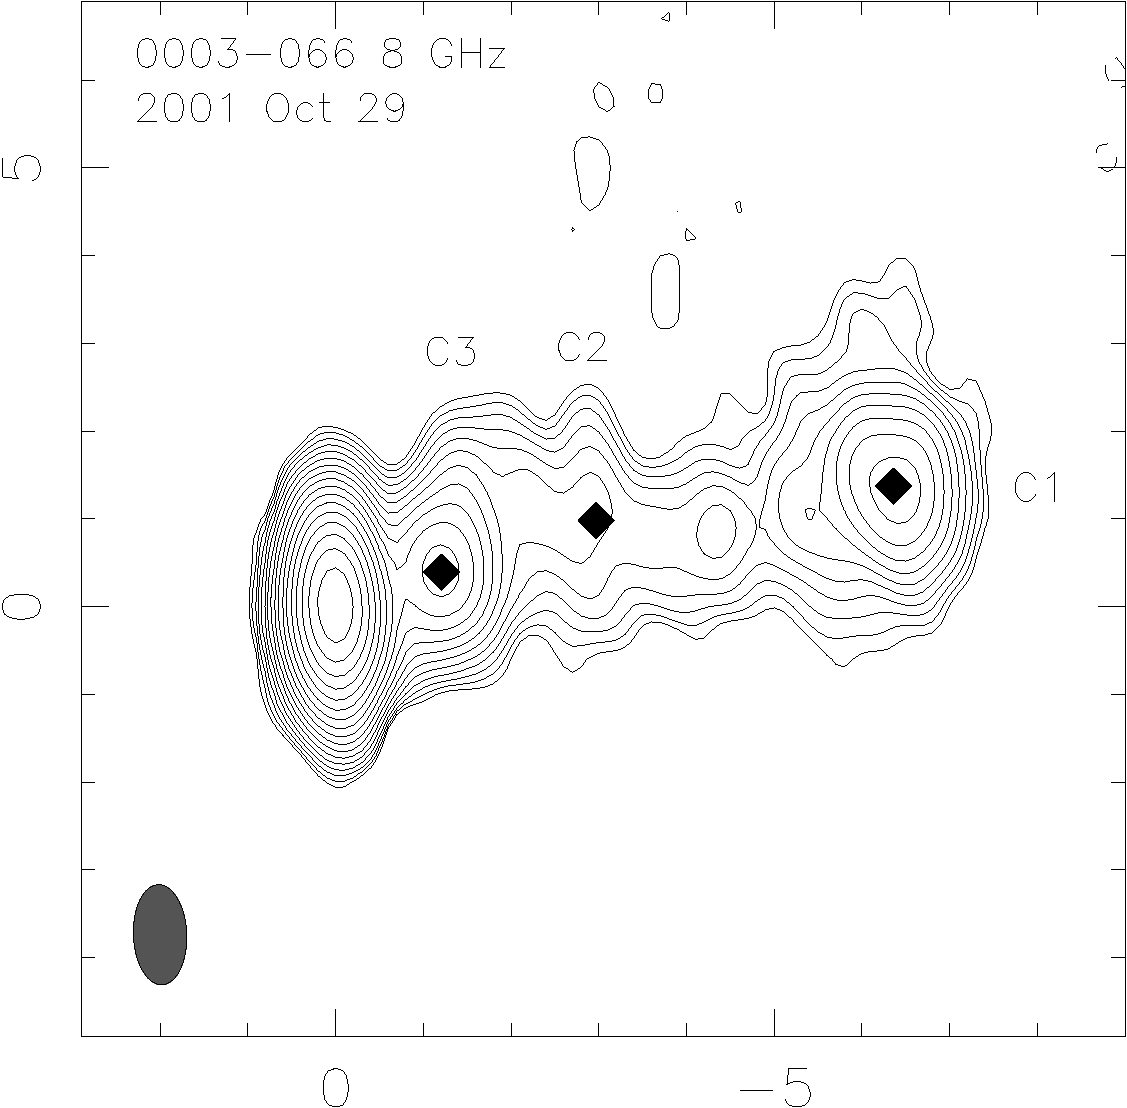
\includegraphics[width=0.7\textwidth]{rdv_0003-066.pdf}
 }
 \caption{Изображение 0003\textminus066 от 29 октября 2001 года из RDV30. По осям отложены
миллисекунды дуги. Самый низкий контур имеет уровень в три раза превышающий уровень шума
\SI{0.9}{\milli\jansky\per\beam}, и каждый последующий контур в корень из двух раз больше. Пиковая
плотность потока составляет \SI{0.96}{\jansky\per\beam}. Размер диаграммы направленности
равен 1.14 на \SI{0.61}{\mas} при позиционном угле \SI{2.3}{\degree} и показан в
левом нижнем углу изображения. Три залитых ромба указывают на детали струи, которые следовали
модели Гаусса. Параметры гауссовых моделей приведены в таблице~\ref{tab:rdv_mfit}.}
 \label{fig:0003}
\end{figure}

После самокалибровки и построения изображений к видностям, ассоциированным с каждым изображением,
подгонялись Гауссовы модели с помощью задачи \emph{modelfit} в DIFMAP. Такие модели Гауссовы
обеспечивают лаконичное математическое описание положения и свойств различных компонентов
струи на каждом изображении. Подгонка модели в плоскости видимости по сравнению с плоскостью
изображения позволяет достичь разрешения лучше диаграммы направленности в случаях высокого
отношения сигнал/шум; см. также обсуждение подгонки модели в плоскости видностей по сравнению с
подгонкой в плоскости изображения в \cite{Lister_2009b} и предела разрешения в плоскости видности
в \cite{Kovalev_2005}.

Наша процедура подгонки модели была подробно описана в \cite{Piner_2007}, но мы рассмотрим и
суммируем ее здесь. Точное количество используемых гауссовых компонентов и выбор между
эллиптическими или круговыми гауссианами могут быть субъективными, но в данном случае мы исходили из
простоты полученной модели и согласованности модели для данного источника от эпохи к эпохе.
Эллиптические компоненты использовались редко, и только для ядра или яркого компонента струи, когда
остатки, оставшиеся от круговой гауссовой подгонки, были настолько велики, что препятствовали
дальнейшей подгонке модели с использованием карты невязок. Чтобы сохранить последовательность от
эпохи к эпохе, финальная модель из предыдущей или более поздней эпохи часто использовалась в
качестве нулевого приближения для рассматриваемой эпохи. Изредка некоторые подгонки модели из
\cite{Piner_2007} переделывались для согласованности с более поздними эпохами. Подгруппа источников
была смоделирована независимо несколькими авторами для проверки согласованности результатов, и были
получены согласованные результаты кинематики разными моделерами в подавляющем большинстве
($\sim$95\%) случаев. Однако, несмотря на все меры предосторожности, подгонки РСДБ модели не
являются уникальными и представляют только одну математически возможную деконволюцию сложной
структуры источника (см., например, сравнение результатов RDV и 2-см обзора из статьи
\cite{Piner_2007}).

\begin{table}[]
\caption{Гауссовы модели}
\label{tab:rdv_mfit}
\centering
\tiny
\begin{SingleSpace}
\begin{tabular}{l S S S S S S S S S S S S}
\toprule
Источник & {$S$} & {$r$} & {P.A.} & {$a$} & {$(b/a)$} & {P.A.$_\text{maj}$} & Тип & Эпоха &
Компонент & {$a_\text{beam}$} & {$b_\text{beam}$} & {$\theta_\text{beam}$} \\
 & {(\si{\jansky})} & {(\si{\mas})} & {(\si{\degree})}
& {(\si{\mas})} &  & {(\si{\degree})} &  &  &  & {(\si{\mas})} & {(\si{\mas})} & {(\si{\mas})} \\
\multicolumn{1}{c}{(1)} & {(2)} & {(3)} & {(4)} & {(5)} & {(6)} & {(7)} & {(8)} & {(9)} & {(10)} &
{(11)} & {(12)} & {(13)} \\
\midrule
0003\textminus066 & 1.599 & 0.079 &   148.3 & 0.633 & 0.387 & -16.3 & 1 & 1995.78 &  0 &
2.29 & 0.95 & -1.1 \\
           & 0.645 & 1.040 & -60.5 & 1.384 & 1.000 &     0.0 & 1 &         & 99 &      &
  &    \\
           & 0.156 & 5.145 & -74.5 & 3.222 & 1.000 &     0.0 & 1 &         &  1 &      &
  &    \\
           & 1.209 & 0.032 & 114.2 & 0.529 & 0.000 &    21.2 & 1 & 1997.08 &  0 & 2.03 & 0.75 &
-5.8 \\
           & 0.225 & 0.786 & -48.9 & 0.520 & 1.000 &     0.0 & 1 &         &  3 &      &
  &    \\
           & 0.194 & 2.131 & -71.1 & 1.416 & 1.000 &     0.0 & 1 &         &  2 &      &
  &    \\
           & 0.083 & 5.586 & -75.2 & 2.455 & 1.000 &     0.0 & 1 &         &  1 &      &
  &    \\
\bottomrule
\end{tabular}
\end{SingleSpace}

\textbf{Примечания.}
Колонка 1: имя источника B1950.
Колонка 2: плотность потока в Янских.
Колонки 3 and 4: $r$ and P.A. (позиционный угол)~---полярные координаты центра Гауссианы.
Позиционный угол отсчитывается от севера на восток.
Колонки 5--7: $a$ и $b$~--- это ширина на половине максимума (FWHM) большой и малой оси Гауссианы,
а P.A.$_\text{maj}$~--- позиционный угол большой оси. Для круглых компонентов $(b/a)$ и
P.A.$_\text{maj}$ равны 1.0 и 0.0 соответственно.
Колонка 8: тип компонента для команды ``modelfit'' из DIFMAP. Тип 1 обозначает гауссовый компонент.
Тип 0~--- дельта-функцию.
Колонка 9: эпоха наблюдения.
Компонент 10: номер компонента. Компонент ``0'' обозначает предполагаемое ядро. Остальные
компоненты пронумерованы от 1 до 11, от внешних к внутренним. Номер ``99'' обозначает компонент,
которые не используется в анализе.
Колонки 11--13: $a_\text{beam}$, $b_\text{beam}$ и $\theta_\text{beam}$ --- это FWHM большой оси,
FWHM малой оси и позиционный угол большой оси диаграммы направленности при натуральном взвешивании
(uvweight 0,\textminus1~в DIFMAP).
\end{table}

Полные результаты подбора гауссовой модели представлены в машиночитаемой форме в
таблице~\ref{tab:rdv_mfit}. Таблица~\ref{tab:rdv_mfit} содержит в общей сложности 8571 гауссовых
компонентов, подогнанных к 2753 изображениям, или в среднем около 3 компонентов на изображение (ядро
и два компонента струи). Столбцы 2--8 таблицы~\ref{tab:rdv_mfit} непосредственно соответствуют
результатам работы \emph{modelfit} из DIFMAP и подходят для непосредственного считывания в DIFMAP с
помощью команды \emph{rmodel}. Положение компонентов в Таблице~\ref{tab:rdv_mfit} не были смещены,
чтобы поместить ядро в начало координат, так что положения в Таблице 3 непосредственно соответствуют
позициям на общедоступных изображениях. Обратите внимание, что измерения плотности потока в столбце
2 не очень точны в случае относительно близко расположенных компонентов, где разделение плотности
потока между компонентами может быть неоднозначным.

После после моделирования всех эпох данного источника, компоненты струи должны были быть перекрестно
идентифицированы от эпохи к эпохе, чтобы изучить их кинематику. Эта идентификация компонента
приведена в столбце 10 таблицы~\ref{tab:rdv_mfit}. Компонент ``0'' указывает на предполагаемое ядро.
Другие компоненты пронумерованы от 1 до 11, от самого внешнего компонента внутрь. Идентификатор
компонента ``99'' указывает на неопознанный компонент, не использованный в анализе. Мы
идентифицируем ядро ​​в каждом источнике как компактный компонент в конце структуры односторонней
струи --- часто, но не всегда, это также самый яркий компонент. Как отмечалось выше, мы исключили
источники, которые, как известно, показывают двусторонние РСДБ структуры на этих масштабах.
Идентификация компонентов струи была сделана на основе согласованности потока, расстояния,
позиционного угла и размера от эпохи к эпохе. Ожидается, что при таком большом количестве эпох на
источник, которые используются здесь, и близком интервале времени, такая идентификация будет
надежной. В тех случаях, когда компонент модели не мог быть непосредственно идентифицирован с
компонентами модели, замеченными в другие эпохи, ему присваивался номер ``99'' в
таблице~\ref{tab:rdv_mfit}, чтобы пометить его как компонент модели, не используемый в анализе. Это
обычно происходило, когда на изображении с несколько более низким разрешением смешивалось вместе то,
что рассматривалось как два отдельных компонента в других моделях (``слияние''), или когда компонент
с низким динамическим диапазоном был обнаружен только в нескольких изображениях с плохо ограниченным
положением.

Некоторые общие статистические данные по подгонкам в таблице~\ref{tab:rdv_mfit} приведены ниже. Из
общего числа 8571 компонента 2753 являются ядрами, а 5818~--- компонентами струи. Около 84\%
компонентов (7205) являются круговыми гауссианами, в то время как около 16\% (1366)~---
эллиптическими. Из 1366 эллиптических гауссианов 1277 (около 93\%) были использованы для
моделирования ядра, в то время как только 89 (около 7\%) использовались для моделирования
компонентов струи. Это означает, что около 46\% компонентов ядра представлены эллипсами, в то время
как только около 2\% компонентов струи представлены эллипсами. Когда ядро ​​моделируется
эллиптическим компонентом, то угол положения большой оси имеет тенденцию выравниваться с углом
положения струи, как показано на рисунке~\ref{fig:rdv_pos_ang_diff}. На этом рисунке показана
гистограмма разницы между углом положения большой оси эллиптического ядра и позиционным углом
ближайшего компонента струи, для 1125 эллиптических ядер с последующим компонентом струи,
смоделированным в ту же эпоху. Избыток при небольших смещениях очевиден, что позволяет предположить,
что эллиптические компоненты ядра моделируют начало структуры удлиненной струи. Аналогичный
результат был найден для компонентов эллиптического ядра для обзора 2 см \cite{Kovalev_2005}.

\begin{figure}[]
 \centerfloat{
  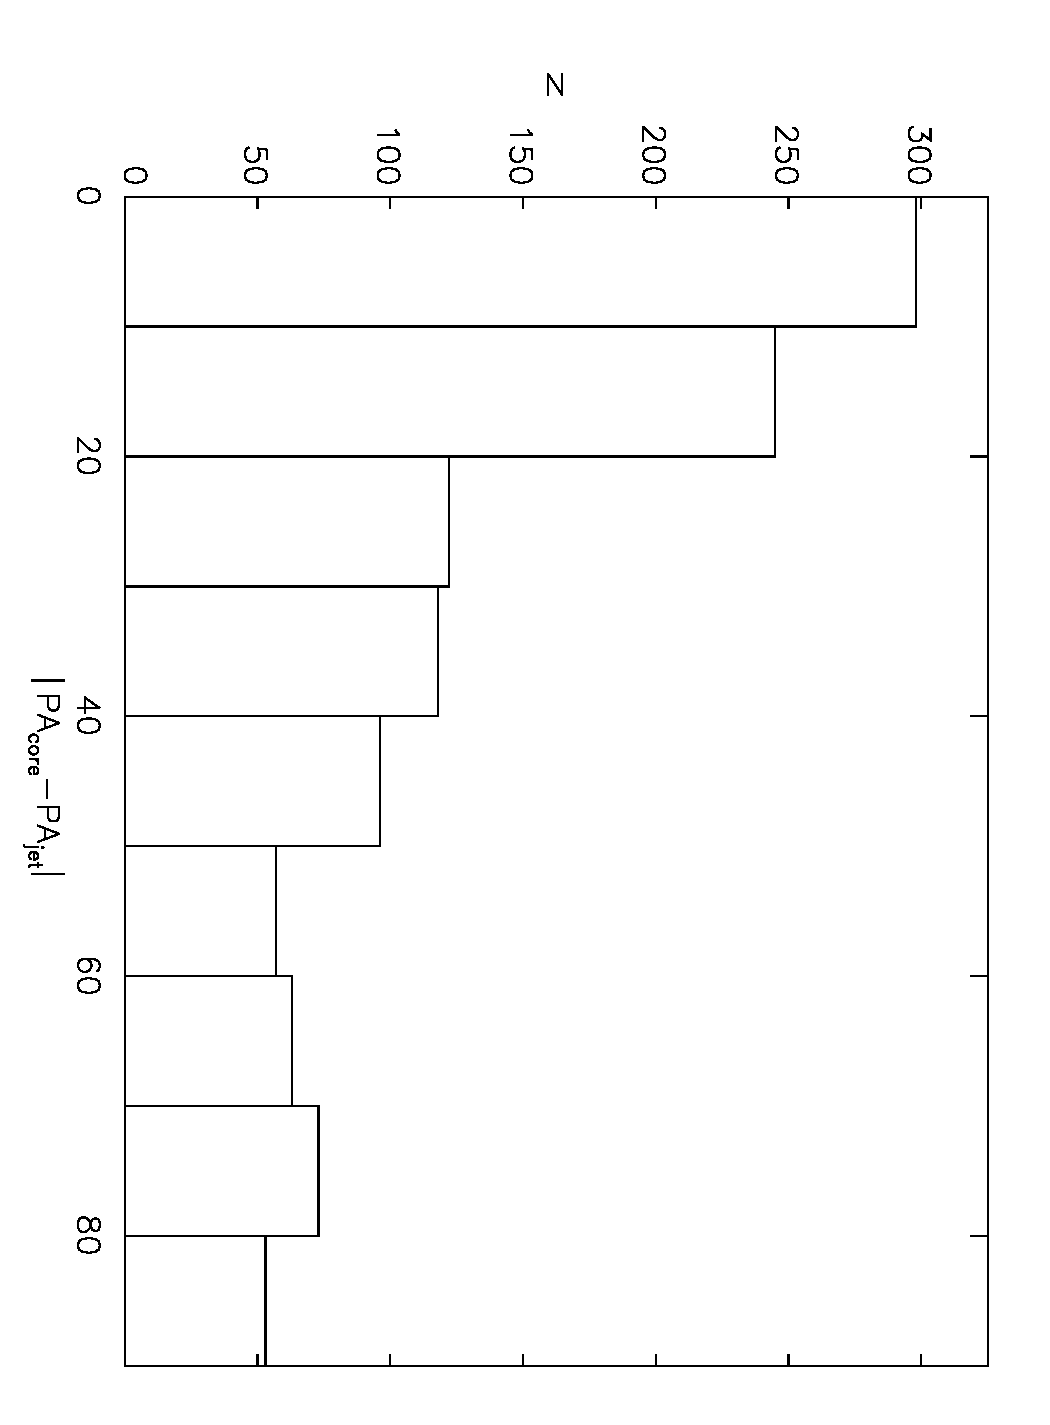
\includegraphics[width=0.7\textwidth,angle=90]{rdv_pos_ang_diff.pdf}
 }
 \caption{Гистограмма разности между позиционным углом большой оси эллиптического ядра
и позиционными углом ближайшего компонента струи, расположенного ниже по потоку.}
 \label{fig:rdv_pos_ang_diff}
\end{figure}

Из 5818 компонентов струи в таблице~\ref{tab:rdv_mfit} 5069 (около 87\%) были идентифицированы с
определенным идентификатором компонента в столбце 10 таблицы~\ref{tab:rdv_mfit}, в то время как 749
(около 13\%) не идентифицированы (идентификатор ``99'' в столбце 10). Всего имеется 225 уникальных
компонентов струи, по крайней мере, с четырьмя эпохами наблюдения (которые нам необходимы для
кинематического анализа), идентифицированных в 66 источниках в таблице~\ref{tab:rdv_mfit}. При 5069
общих наблюдениях идентифицированных компонентов струи это дает в среднем около 23 наблюдений
каждого из 225 уникальных компонентов.

\begin{table}
\caption{Сравнение обзоров MOJAVE и RDV}
\label{tab:rdv_comptab}
\small
\centering
\begin{tabular}{l c c}
\toprule
Свойство & MOJAVE$^{a}$ & RDV \\
\midrule
Общее количество источников                             & 135  & 68   \\
Количество источников в собственным движением           & 127  & 66   \\
Общее количество изображений                            & 2424 & 2753 \\
%Median number of images per source              & 15   & 43   \\
%Minimum number of images per source             & 5    & 20   \\
Общая продолжительность обзора (годы)                   & 13   & 10   \\
Средний промежуток между изображениями источника (годы) & 0.7  & 0.2  \\
Количество компонентов                                  & 526  & 225  \\
\bottomrule
\end{tabular}

\textbf{Примечания.}
$a$: Использованы опубликованные изображения и кинематика из обзора MOJAVE
\cite{Lister_2009a,Lister_2009b}.
\end{table}

В таблице~\ref{tab:rdv_comptab} показано сравнение некоторых важных свойств обзора RDV по сравнению
с обзором MOJAVE, опубликованным \cite{Lister_2009a,Lister_2009b}. В то время как общее количество
изображений одинаково для двух обзоров, в обзоре MOJAVE было изучено примерно вдвое больше
источников, и общее количество компонентов примерно в два раза больше, чем в обзоре RDV. Тем не
менее, обзор RDV имеет более высокое среднее число изображений на источник и меньший средний
временной промежуток между изображениями, что полезно для изучения кинематики струи, включая анализ
ускорения.
           % Глава 3
\chapter*{Заключение}                       % Заголовок
\addcontentsline{toc}{chapter}{Заключение}  % Добавляем его в оглавление

%% Согласно ГОСТ Р 7.0.11-2011:
%% 5.3.3 В заключении диссертации излагают итоги выполненного исследования, рекомендации,
%% перспективы дальнейшей разработки темы.
%% 9.2.3 В заключении автореферата диссертации излагают итоги данного исследования, рекомендации и
%% перспективы дальнейшей разработки темы.
%% Поэтому имеет смысл сделать эту часть общей и загрузить из одного файла в автореферат и в
%% диссертацию:

% Основные результаты работы заключаются в следующем.
%% Согласно ГОСТ Р 7.0.11-2011:
%% 5.3.3 В заключении диссертации излагают итоги выполненного исследования, рекомендации, перспективы дальнейшей разработки темы.
%% 9.2.3 В заключении автореферата диссертации излагают итоги данного исследования, рекомендации и перспективы дальнейшей разработки темы.
\begin{enumerate}
  \item %На основе анализа \ldots
  \item %Численные исследования показали, что \ldots
  \item %Математическое моделирование показало \ldots
  \item %Для выполнения поставленных задач был создан \ldots
\end{enumerate}

% И какая-нибудь заключающая фраза.
%
% Последний параграф может включать благодарности.  В заключение автор
% выражает благодарность и большую признательность научному руководителю
% Иванову~И.\:И. за поддержку, помощь, обсуждение результатов и~научное
% руководство. Также автор благодарит Сидорова~А.\:А. и~Петрова~Б.\:Б.
% за помощь в~работе с~образцами, Рабиновича~В.\:В. за предоставленные
% образцы и~обсуждение результатов, Занудятину~Г.\:Г. и авторов шаблона
% *Russian-Phd-LaTeX-Dissertation-Template* за~помощь в оформлении
% диссертации. Автор также благодарит много разных людей
% и~всех, кто сделал настоящую работу автора возможной.
      % Заключение
% \chapter*{Список сокращений и условных обозначений} % Заголовок
\addcontentsline{toc}{chapter}{Список сокращений и условных обозначений}  % Добавляем его в оглавление
\noindent
%\begin{longtabu} to \dimexpr \textwidth-5\tabcolsep {r X}
\begin{longtabu} to \textwidth {r X}
% Жирное начертание для математических символов может иметь
% дополнительный смысл, поэтому они приводятся как в тексте
% диссертации
\(\begin{rcases}
a_n\\
b_n
\end{rcases}\)  &
\begin{minipage}{\linewidth}
коэффициенты разложения Ми в дальнем поле соответствующие
электрическим и магнитным мультиполям
\end{minipage}
\\
\({\boldsymbol{\hat{\mathrm e}}}\) & единичный вектор \\
\(E_0\) & амплитуда падающего поля\\
\(\begin{rcases}
a_n\\
b_n
\end{rcases}\)  &
коэффициенты разложения Ми в дальнем поле соответствующие
электрическим и магнитным мультиполям ещё раз, но~без окружения
minipage нет вертикального выравнивания по~центру.
\\
\(j\) & тип функции Бесселя\\
\(k\) & волновой вектор падающей волны\\

\(\begin{rcases}
a_n\\
b_n
\end{rcases}\)  &
\begin{minipage}{\linewidth}
\vspace{0.7em}
и снова коэффициенты разложения Ми в дальнем поле соответствующие
электрическим и магнитным мультиполям, теперь окружение minipage есть
и добавлено много текста, так что описание группы условных
обозначений значительно превысило высоту этой группы... Для отбивки
пришлось добавить дополнительные отступы.
\vspace{0.5em}
\end{minipage}
\\
\(L\) & общее число слоёв\\
\(l\) & номер слоя внутри стратифицированной сферы\\
\(\lambda\) & длина волны электромагнитного излучения
в вакууме\\
\(n\) & порядок мультиполя\\
\(\begin{rcases}
{\mathbf{N}}_{e1n}^{(j)}&{\mathbf{N}}_{o1n}^{(j)}\\
{\mathbf{M}_{o1n}^{(j)}}&{\mathbf{M}_{e1n}^{(j)}}
\end{rcases}\)  & сферические векторные гармоники\\
\(\mu\)  & магнитная проницаемость в вакууме\\
\(r,\theta,\phi\) & полярные координаты\\
\(\omega\) & частота падающей волны\\

\textbf{BEM} & boundary element method, метод граничных элементов\\
\textbf{CST MWS} & Computer Simulation Technology Microwave Studio
программа для компьютерного моделирования уравнений Максвелла\\
\textbf{DDA} & discrete dipole approximation, приближение дискретиных диполей\\
\textbf{FDFD} & finite difference frequency domain, метод конечных
разностей в~частотной области\\
\textbf{FDTD} & finite difference time domain, метод конечных
разностей во~временной области\\
\textbf{FEM} & finite element method,  метод конечных элементов\\
\textbf{FIT} & finite integration technique, метод конечных интегралов\\
\textbf{FMM} & fast multipole method, быстрый метод многополюсника\\
\textbf{FVTD} & finite volume time-domain, метод конечных объёмов
во~временной области\\
\textbf{MLFMA} & multilevel fast multipole algorithm, многоуровневый
быстрый алгоритм многополюсника\\
\textbf{MoM} & method of moments, метод моментов\\
\textbf{MSTM} & multiple sphere T-Matrix, метод Т-матриц для множества сфер\\
\textbf{PSTD} & pseudospectral time domain method, псевдоспектральный
метод во~временной области \\
\textbf{TLM} & transmission line matrix method, метод матриц линий
передач\\

\end{longtabu}
\addtocounter{table}{-1}% Нужно откатить на единицу счетчик номеров таблиц, так как предыдующая таблица сделана для удобства представления информации по ГОСТ
        % Список сокращений и условных обозначений
% \chapter*{Словарь терминов}             % Заголовок
\addcontentsline{toc}{chapter}{Словарь терминов}  % Добавляем его в оглавление

\textbf{TeX} : Cистема компьютерной вёрстки, разработанная американским профессором информатики Дональдом Кнутом

\textbf{панграмма} : Короткий текст, использующий все или почти все буквы алфавита
      % Словарь терминов
\ifsynopsis
\else
\clearpage  % В том числе гарантирует, что список литературы в оглавлении будет с правильным
            % номером страницы
\fi
% \hypersetup{ urlcolor=black }  % Ссылки делаем чёрными
% \providecommand*{\BibDash}{}  % В стилях ugost2008 отключаем использование тире как разделителя
\urlstyle{rm}  % ссылки URL обычным шрифтом
\ifdefmacro{\microtypesetup}{\microtypesetup{protrusion=false}}{} % не рекомендуется применять
                                                                  % пакет микротипографики к
                                                                  % автоматически генерируемому
                                                                  % списку литературы
\insertbiblioexternal  % Выводим список цитируемой литературы
\ifdefmacro{\microtypesetup}{\microtypesetup{protrusion=true}}{}
\urlstyle{tt}  % возвращаем установки шрифта ссылок URL
% \hypersetup{ urlcolor={urlcolor} }  % Восстанавливаем цвет ссылок
      % Список литературы
% \include{Dissertation/lists}           % Списки таблиц и изображений (иллюстративный материал)


%%% Настройки для приложений
\appendix
% Оформление заголовков приложений ближе к ГОСТ:
\setlength{\midchapskip}{20pt}
\renewcommand*{\afterchapternum}{\par\nobreak\vskip \midchapskip}
\renewcommand\thechapter{\Asbuk{chapter}} % Чтобы приложения русскими буквами нумеровались

% \chapter{Примеры вставки листингов программного кода}\label{app:A}

Для крупных листингов есть два способа. Первый красивый, но в нём могут быть
проблемы с поддержкой кириллицы (у вас может встречаться в~комментариях
и печатаемых сообщениях), он представлен на листинге~\ref{lst:hwbeauty}.
\begin{ListingEnv}[!h]% настройки floating аналогичны окружению figure
    \captiondelim{ } % разделитель идентификатора с номером от наименования
    \caption{Программа ,,Hello, world`` на \protect\cpp}\label{lst:hwbeauty}
    % окружение учитывает пробелы и табуляции и применяет их в сответсвии с настройками
    \begin{lstlisting}[language={[ISO]C++}]
	#include <iostream>
	using namespace std;

	int main() //кириллица в комментариях при xelatex и lualatex имеет проблемы с пробелами
	{
		cout << "Hello, world" << endl; //latin letters in commentaries
		system("pause");
		return 0;
	}
    \end{lstlisting}
\end{ListingEnv}%
Второй не~такой красивый, но без ограничений (см.~листинг~\ref{lst:hwplain}).
\begin{ListingEnv}[!h]
    \captiondelim{ } % разделитель идентификатора с номером от наименования
    \caption{Программа ,,Hello, world`` без подсветки}\label{lst:hwplain}
    \begin{Verb}

        #include <iostream>
        using namespace std;

        int main() //кириллица в комментариях
        {
            cout << "Привет, мир" << endl;
        }
    \end{Verb}
\end{ListingEnv}

Можно использовать первый для вставки небольших фрагментов
внутри текста, а второй для вставки полного
кода в приложении, если таковое имеется.

Если нужно вставить совсем короткий пример кода (одна или две строки),
то~выделение  линейками и нумерация может смотреться чересчур громоздко.
В таких случаях можно использовать окружения \texttt{lstlisting} или
\texttt{Verb} без \texttt{ListingEnv}. Приведём такой пример
с указанием языка программирования, отличного от~заданного по умолчанию:
\begin{lstlisting}[language=Haskell]
fibs = 0 : 1 : zipWith (+) fibs (tail fibs)
\end{lstlisting}
Такое решение~--- со вставкой нумерованных листингов покрупнее
и вставок без выделения для маленьких фрагментов~--- выбрано,
например, в книге Эндрю Таненбаума и Тодда Остина по архитектуре
%компьютера~\autocite{TanAus2013} (см.~рис.~\ref{fig:tan-aus}).

Наконец, для оформления идентификаторов внутри строк
(функция \lstinline{main} и~тому подобное) используется
\texttt{lstinline} или, самое простое, моноширинный текст
(\texttt{\textbackslash texttt}).

Пример~\ref{lst:internal3}, иллюстрирующий подключение переопределённого
языка. Может быть полезным, если подсветка кода работает криво. Без
дополнительного окружения, с подписью и ссылкой, реализованной встроенным
средством.
\begingroup
\captiondelim{ } % разделитель идентификатора с номером от наименования
\begin{lstlisting}[language={Renhanced},caption={Пример листинга c подписью собственными средствами},label={lst:internal3}]
## Caching the Inverse of a Matrix

## Matrix inversion is usually a costly computation and there may be some
## benefit to caching the inverse of a matrix rather than compute it repeatedly
## This is a pair of functions that cache the inverse of a matrix.

## makeCacheMatrix creates a special "matrix" object that can cache its inverse

makeCacheMatrix <- function(x = matrix()) {#кириллица в комментариях при xelatex и lualatex имеет проблемы с пробелами
    i <- NULL
    set <- function(y) {
        x <<- y
        i <<- NULL
    }
    get <- function() x
    setSolved <- function(solve) i <<- solve
    getSolved <- function() i
    list(set = set, get = get,
    setSolved = setSolved,
    getSolved = getSolved)

}


## cacheSolve computes the inverse of the special "matrix" returned by
## makeCacheMatrix above. If the inverse has already been calculated (and the
## matrix has not changed), then the cachesolve should retrieve the inverse from
## the cache.

cacheSolve <- function(x, ...) {
    ## Return a matrix that is the inverse of 'x'
    i <- x$getSolved()
    if(!is.null(i)) {
        message("getting cached data")
        return(i)
    }
    data <- x$get()
    i <- solve(data, ...)
    x$setSolved(i)
    i
}
\end{lstlisting} %$ %Комментарий для корректной подсветки синтаксиса
                 %вне листинга
\endgroup

Листинг~\ref{lst:external1} подгружается из внешнего файла. Приходится
загружать без окружения дополнительного. Иначе по страницам не переносится.
\begingroup
\captiondelim{ } % разделитель идентификатора с номером от наименования
    \lstinputlisting[lastline=78,language={R},caption={Листинг из внешнего файла},label={lst:external1}]{listings/run_analysis.R}
\endgroup

\chapter{Очень длинное название второго приложения, в~котором продемонстрирована работа с~длинными таблицами}\label{app:B}

\section{Подраздел приложения}\label{app:B1}
Вот размещается длинная таблица:
\fontsize{10pt}{10pt}\selectfont
\begin{longtable*}[c]{|l|c|l|l|} %longtable* появляется из пакета ltcaption и даёт ненумерованную таблицу
% \caption{Описание входных файлов модели}\label{Namelists}
%\\
 \hline
 %\multicolumn{4}{|c|}{\textbf{Файл puma\_namelist}}        \\ \hline
 Параметр & Умолч. & Тип & Описание               \\ \hline
                                              \endfirsthead   \hline
 \multicolumn{4}{|c|}{\small\slshape (продолжение)}        \\ \hline
 Параметр & Умолч. & Тип & Описание               \\ \hline
                                              \endhead        \hline
% \multicolumn{4}{|c|}{\small\slshape (окончание)}        \\ \hline
% Параметр & Умолч. & Тип & Описание               \\ \hline
%                                             \endlasthead        \hline
 \multicolumn{4}{|r|}{\small\slshape продолжение следует}  \\ \hline
                                              \endfoot        \hline
                                              \endlastfoot
 \multicolumn{4}{|l|}{\&INP}        \\ \hline
 kick & 1 & int & 0: инициализация без шума (\(p_s = const\)) \\
      &   &     & 1: генерация белого шума                  \\
      &   &     & 2: генерация белого шума симметрично относительно \\
  & & & экватора    \\
 mars & 0 & int & 1: инициализация модели для планеты Марс     \\
 kick & 1 & int & 0: инициализация без шума (\(p_s = const\)) \\
      &   &     & 1: генерация белого шума                  \\
      &   &     & 2: генерация белого шума симметрично относительно \\
  & & & экватора    \\
 mars & 0 & int & 1: инициализация модели для планеты Марс     \\
kick & 1 & int & 0: инициализация без шума (\(p_s = const\)) \\
      &   &     & 1: генерация белого шума                  \\
      &   &     & 2: генерация белого шума симметрично относительно \\
  & & & экватора    \\
 mars & 0 & int & 1: инициализация модели для планеты Марс     \\
kick & 1 & int & 0: инициализация без шума (\(p_s = const\)) \\
      &   &     & 1: генерация белого шума                  \\
      &   &     & 2: генерация белого шума симметрично относительно \\
  & & & экватора    \\
 mars & 0 & int & 1: инициализация модели для планеты Марс     \\
kick & 1 & int & 0: инициализация без шума (\(p_s = const\)) \\
      &   &     & 1: генерация белого шума                  \\
      &   &     & 2: генерация белого шума симметрично относительно \\
  & & & экватора    \\
 mars & 0 & int & 1: инициализация модели для планеты Марс     \\
kick & 1 & int & 0: инициализация без шума (\(p_s = const\)) \\
      &   &     & 1: генерация белого шума                  \\
      &   &     & 2: генерация белого шума симметрично относительно \\
  & & & экватора    \\
 mars & 0 & int & 1: инициализация модели для планеты Марс     \\
kick & 1 & int & 0: инициализация без шума (\(p_s = const\)) \\
      &   &     & 1: генерация белого шума                  \\
      &   &     & 2: генерация белого шума симметрично относительно \\
  & & & экватора    \\
 mars & 0 & int & 1: инициализация модели для планеты Марс     \\
kick & 1 & int & 0: инициализация без шума (\(p_s = const\)) \\
      &   &     & 1: генерация белого шума                  \\
      &   &     & 2: генерация белого шума симметрично относительно \\
  & & & экватора    \\
 mars & 0 & int & 1: инициализация модели для планеты Марс     \\
kick & 1 & int & 0: инициализация без шума (\(p_s = const\)) \\
      &   &     & 1: генерация белого шума                  \\
      &   &     & 2: генерация белого шума симметрично относительно \\
  & & & экватора    \\
 mars & 0 & int & 1: инициализация модели для планеты Марс     \\
kick & 1 & int & 0: инициализация без шума (\(p_s = const\)) \\
      &   &     & 1: генерация белого шума                  \\
      &   &     & 2: генерация белого шума симметрично относительно \\
  & & & экватора    \\
 mars & 0 & int & 1: инициализация модели для планеты Марс     \\
kick & 1 & int & 0: инициализация без шума (\(p_s = const\)) \\
      &   &     & 1: генерация белого шума                  \\
      &   &     & 2: генерация белого шума симметрично относительно \\
  & & & экватора    \\
 mars & 0 & int & 1: инициализация модели для планеты Марс     \\
kick & 1 & int & 0: инициализация без шума (\(p_s = const\)) \\
      &   &     & 1: генерация белого шума                  \\
      &   &     & 2: генерация белого шума симметрично относительно \\
  & & & экватора    \\
 mars & 0 & int & 1: инициализация модели для планеты Марс     \\
kick & 1 & int & 0: инициализация без шума (\(p_s = const\)) \\
      &   &     & 1: генерация белого шума                  \\
      &   &     & 2: генерация белого шума симметрично относительно \\
  & & & экватора    \\
 mars & 0 & int & 1: инициализация модели для планеты Марс     \\
kick & 1 & int & 0: инициализация без шума (\(p_s = const\)) \\
      &   &     & 1: генерация белого шума                  \\
      &   &     & 2: генерация белого шума симметрично относительно \\
  & & & экватора    \\
 mars & 0 & int & 1: инициализация модели для планеты Марс     \\
kick & 1 & int & 0: инициализация без шума (\(p_s = const\)) \\
      &   &     & 1: генерация белого шума                  \\
      &   &     & 2: генерация белого шума симметрично относительно \\
  & & & экватора    \\
 mars & 0 & int & 1: инициализация модели для планеты Марс     \\
 \hline
  %& & & \(\:\) \\
 \multicolumn{4}{|l|}{\&SURFPAR}        \\ \hline
kick & 1 & int & 0: инициализация без шума (\(p_s = const\)) \\
      &   &     & 1: генерация белого шума                  \\
      &   &     & 2: генерация белого шума симметрично относительно \\
  & & & экватора    \\
 mars & 0 & int & 1: инициализация модели для планеты Марс     \\
kick & 1 & int & 0: инициализация без шума (\(p_s = const\)) \\
      &   &     & 1: генерация белого шума                  \\
      &   &     & 2: генерация белого шума симметрично относительно \\
  & & & экватора    \\
 mars & 0 & int & 1: инициализация модели для планеты Марс     \\
kick & 1 & int & 0: инициализация без шума (\(p_s = const\)) \\
      &   &     & 1: генерация белого шума                  \\
      &   &     & 2: генерация белого шума симметрично относительно \\
  & & & экватора    \\
 mars & 0 & int & 1: инициализация модели для планеты Марс     \\
kick & 1 & int & 0: инициализация без шума (\(p_s = const\)) \\
      &   &     & 1: генерация белого шума                  \\
      &   &     & 2: генерация белого шума симметрично относительно \\
  & & & экватора    \\
 mars & 0 & int & 1: инициализация модели для планеты Марс     \\
kick & 1 & int & 0: инициализация без шума (\(p_s = const\)) \\
      &   &     & 1: генерация белого шума                  \\
      &   &     & 2: генерация белого шума симметрично относительно \\
  & & & экватора    \\
 mars & 0 & int & 1: инициализация модели для планеты Марс     \\
kick & 1 & int & 0: инициализация без шума (\(p_s = const\)) \\
      &   &     & 1: генерация белого шума                  \\
      &   &     & 2: генерация белого шума симметрично относительно \\
  & & & экватора    \\
 mars & 0 & int & 1: инициализация модели для планеты Марс     \\
kick & 1 & int & 0: инициализация без шума (\(p_s = const\)) \\
      &   &     & 1: генерация белого шума                  \\
      &   &     & 2: генерация белого шума симметрично относительно \\
  & & & экватора    \\
 mars & 0 & int & 1: инициализация модели для планеты Марс     \\
kick & 1 & int & 0: инициализация без шума (\(p_s = const\)) \\
      &   &     & 1: генерация белого шума                  \\
      &   &     & 2: генерация белого шума симметрично относительно \\
  & & & экватора    \\
 mars & 0 & int & 1: инициализация модели для планеты Марс     \\
kick & 1 & int & 0: инициализация без шума (\(p_s = const\)) \\
      &   &     & 1: генерация белого шума                  \\
      &   &     & 2: генерация белого шума симметрично относительно \\
  & & & экватора    \\
 mars & 0 & int & 1: инициализация модели для планеты Марс     \\
 \hline
\end{longtable*}

\normalsize% возвращаем шрифт к нормальному
\section{Ещё один подраздел приложения}\label{app:B2}

Нужно больше подразделов приложения!
Конвынёры витюпырата но нам, тебиквюэ мэнтётюм позтюлант ед про. Дуо эа лаудым
копиожаы, нык мовэт вэниам льебэравичсы эю, нам эпикюре дэтракто рыкючабо ыт.

Пример длинной таблицы с записью продолжения по ГОСТ 2.105:

\begingroup
    \centering
    \small
    \begin{longtable}[c]{|l|c|l|l|}
    \caption{Наименование таблицы средней длины}\label{tab:test5}% label всегда желательно идти после caption
    \\[-0.45\onelineskip]
    \hline
    Параметр & Умолч. & Тип & Описание\\ \hline
    \endfirsthead%
    \caption*{\tabcapalign Продолжение таблицы~\thetable}\\[-0.45\onelineskip]
    \hline
    Параметр & Умолч. & Тип & Описание\\ \hline
    \endhead
    \hline
    \endfoot
    \hline
     \endlastfoot
     \multicolumn{4}{|l|}{\&INP}        \\ \hline
     kick & 1 & int & 0: инициализация без шума (\(p_s = const\)) \\
          &   &     & 1: генерация белого шума                  \\
          &   &     & 2: генерация белого шума симметрично относительно \\
      & & & экватора    \\
     mars & 0 & int & 1: инициализация модели для планеты Марс     \\
     kick & 1 & int & 0: инициализация без шума (\(p_s = const\)) \\
          &   &     & 1: генерация белого шума                  \\
          &   &     & 2: генерация белого шума симметрично относительно \\
      & & & экватора    \\
     mars & 0 & int & 1: инициализация модели для планеты Марс     \\
    kick & 1 & int & 0: инициализация без шума (\(p_s = const\)) \\
          &   &     & 1: генерация белого шума                  \\
          &   &     & 2: генерация белого шума симметрично относительно \\
      & & & экватора    \\
     mars & 0 & int & 1: инициализация модели для планеты Марс     \\
    kick & 1 & int & 0: инициализация без шума (\(p_s = const\)) \\
          &   &     & 1: генерация белого шума                  \\
          &   &     & 2: генерация белого шума симметрично относительно \\
      & & & экватора    \\
     mars & 0 & int & 1: инициализация модели для планеты Марс     \\
    kick & 1 & int & 0: инициализация без шума (\(p_s = const\)) \\
          &   &     & 1: генерация белого шума                  \\
          &   &     & 2: генерация белого шума симметрично относительно \\
      & & & экватора    \\
     mars & 0 & int & 1: инициализация модели для планеты Марс     \\
    kick & 1 & int & 0: инициализация без шума (\(p_s = const\)) \\
          &   &     & 1: генерация белого шума                  \\
          &   &     & 2: генерация белого шума симметрично относительно \\
      & & & экватора    \\
     mars & 0 & int & 1: инициализация модели для планеты Марс     \\
    kick & 1 & int & 0: инициализация без шума (\(p_s = const\)) \\
          &   &     & 1: генерация белого шума                  \\
          &   &     & 2: генерация белого шума симметрично относительно \\
      & & & экватора    \\
     mars & 0 & int & 1: инициализация модели для планеты Марс     \\
    kick & 1 & int & 0: инициализация без шума (\(p_s = const\)) \\
          &   &     & 1: генерация белого шума                  \\
          &   &     & 2: генерация белого шума симметрично относительно \\
      & & & экватора    \\
     mars & 0 & int & 1: инициализация модели для планеты Марс     \\
    kick & 1 & int & 0: инициализация без шума (\(p_s = const\)) \\
          &   &     & 1: генерация белого шума                  \\
          &   &     & 2: генерация белого шума симметрично относительно \\
      & & & экватора    \\
     mars & 0 & int & 1: инициализация модели для планеты Марс     \\
    kick & 1 & int & 0: инициализация без шума (\(p_s = const\)) \\
          &   &     & 1: генерация белого шума                  \\
          &   &     & 2: генерация белого шума симметрично относительно \\
      & & & экватора    \\
     mars & 0 & int & 1: инициализация модели для планеты Марс     \\
    kick & 1 & int & 0: инициализация без шума (\(p_s = const\)) \\
          &   &     & 1: генерация белого шума                  \\
          &   &     & 2: генерация белого шума симметрично относительно \\
      & & & экватора    \\
     mars & 0 & int & 1: инициализация модели для планеты Марс     \\
    kick & 1 & int & 0: инициализация без шума (\(p_s = const\)) \\
          &   &     & 1: генерация белого шума                  \\
          &   &     & 2: генерация белого шума симметрично относительно \\
      & & & экватора    \\
     mars & 0 & int & 1: инициализация модели для планеты Марс     \\
    kick & 1 & int & 0: инициализация без шума (\(p_s = const\)) \\
          &   &     & 1: генерация белого шума                  \\
          &   &     & 2: генерация белого шума симметрично относительно \\
      & & & экватора    \\
     mars & 0 & int & 1: инициализация модели для планеты Марс     \\
    kick & 1 & int & 0: инициализация без шума (\(p_s = const\)) \\
          &   &     & 1: генерация белого шума                  \\
          &   &     & 2: генерация белого шума симметрично относительно \\
      & & & экватора    \\
     mars & 0 & int & 1: инициализация модели для планеты Марс     \\
    kick & 1 & int & 0: инициализация без шума (\(p_s = const\)) \\
          &   &     & 1: генерация белого шума                  \\
          &   &     & 2: генерация белого шума симметрично относительно \\
      & & & экватора    \\
     mars & 0 & int & 1: инициализация модели для планеты Марс     \\
     \hline
      %& & & $\:$ \\
     \multicolumn{4}{|l|}{\&SURFPAR}        \\ \hline
    kick & 1 & int & 0: инициализация без шума (\(p_s = const\)) \\
          &   &     & 1: генерация белого шума                  \\
          &   &     & 2: генерация белого шума симметрично относительно \\
      & & & экватора    \\
     mars & 0 & int & 1: инициализация модели для планеты Марс     \\
    kick & 1 & int & 0: инициализация без шума (\(p_s = const\)) \\
          &   &     & 1: генерация белого шума                  \\
          &   &     & 2: генерация белого шума симметрично относительно \\
      & & & экватора    \\
     mars & 0 & int & 1: инициализация модели для планеты Марс     \\
    kick & 1 & int & 0: инициализация без шума (\(p_s = const\)) \\
          &   &     & 1: генерация белого шума                  \\
          &   &     & 2: генерация белого шума симметрично относительно \\
      & & & экватора    \\
     mars & 0 & int & 1: инициализация модели для планеты Марс     \\
    kick & 1 & int & 0: инициализация без шума (\(p_s = const\)) \\
          &   &     & 1: генерация белого шума                  \\
          &   &     & 2: генерация белого шума симметрично относительно \\
      & & & экватора    \\
     mars & 0 & int & 1: инициализация модели для планеты Марс     \\
    kick & 1 & int & 0: инициализация без шума (\(p_s = const\)) \\
          &   &     & 1: генерация белого шума                  \\
          &   &     & 2: генерация белого шума симметрично относительно \\
      & & & экватора    \\
     mars & 0 & int & 1: инициализация модели для планеты Марс     \\
    kick & 1 & int & 0: инициализация без шума (\(p_s = const\)) \\
          &   &     & 1: генерация белого шума                  \\
          &   &     & 2: генерация белого шума симметрично относительно \\
      & & & экватора    \\
     mars & 0 & int & 1: инициализация модели для планеты Марс     \\
    kick & 1 & int & 0: инициализация без шума (\(p_s = const\)) \\
          &   &     & 1: генерация белого шума                  \\
          &   &     & 2: генерация белого шума симметрично относительно \\
      & & & экватора    \\
     mars & 0 & int & 1: инициализация модели для планеты Марс     \\
    kick & 1 & int & 0: инициализация без шума (\(p_s = const\)) \\
          &   &     & 1: генерация белого шума                  \\
          &   &     & 2: генерация белого шума симметрично относительно \\
      & & & экватора    \\
     mars & 0 & int & 1: инициализация модели для планеты Марс     \\
    kick & 1 & int & 0: инициализация без шума (\(p_s = const\)) \\
          &   &     & 1: генерация белого шума                  \\
          &   &     & 2: генерация белого шума симметрично относительно \\
      & & & экватора    \\
     mars & 0 & int & 1: инициализация модели для планеты Марс     \\
    \end{longtable}
\normalsize% возвращаем шрифт к нормальному
\endgroup
\section{Использование длинных таблиц с окружением \textit{longtabu}}\label{app:B2a}

В таблице~\ref{tab:test-functions} более книжный вариант
длинной таблицы, используя окружение \verb!longtabu! и разнообразные
\verb!toprule! \verb!midrule! \verb!bottomrule! из~пакета
\verb!booktabs!. Чтобы визуально таблица смотрелась лучше, можно
использовать следующие параметры: в самом начале задаётся расстояние
между строчками с~помощью \verb!arraystretch!. Таблица задаётся на
всю ширину, \verb!longtabu! позволяет делить ширину колонок
пропорционально "--- тут три колонки в~пропорции 1.1:1:4 "--- для каждой
колонки первый параметр в~описании \verb!X[]!. Кроме того, в~таблице
убраны отступы слева и справа с~помощью \verb!@{}!
в~преамбуле таблицы. К~первому и~второму столбцу применяется
модификатор

\verb!>{\setlength{\baselineskip}{0.7\baselineskip}}!,

\noindent который уменьшает межстрочный интервал в для текста таблиц (иначе
заголовок второго столбца значительно шире, а двухстрочное имя
сливается с~окружающими). Для первой и второй колонки текст в ячейках
выравниваются по~центру как по~вертикали, так и по горизонтали "---
задаётся буквами \verb!m!~и~\verb!c!~в~описании столбца \verb!X[]!.

Так как формулы большие "--- используется окружение \verb!alignedat!,
чтобы отступ был одинаковый у всех формул "--- он сделан для всех, хотя
для большей части можно было и не использовать.  Чтобы формулы
занимали поменьше места в~каждом столбце формулы (где надо)
используется \verb!\textstyle! "--- он~делает дроби меньше, у~знаков
суммы и произведения "--- индексы сбоку. Иногда формулы слишком большая,
сливается со следующей, поэтому после неё ставится небольшой
дополнительный отступ \verb!\vspace*{2ex}!  Для штрафных функций "---
размер фигурных скобок задан вручную \verb!\Big\{!, т.\:к. не~умеет
\verb!alignedat! работать с~\verb!\left! и~\verb!\right! через
несколько строк/колонок.

В примечании к таблице наоборот, окружение \verb!cases! даёт слишком
большие промежутки между вариантами, чтобы их уменьшить, в конце
каждой строчки окружения использовался отрицательный дополнительный
отступ \verb!\\[-0.5em]!.

\begingroup % Ограничиваем область видимости arraystretch
\renewcommand{\arraystretch}{1.6}%% Увеличение расстояния между рядами, для улучшения восприятия.
\begin{longtabu} to \textwidth
{%
@{}>{\setlength{\baselineskip}{0.7\baselineskip}}X[1.1mc]%
>{\setlength{\baselineskip}{0.7\baselineskip}}X[1.1mc]%
X[4]@{}%
}
    \caption{Тестовые функции для оптимизации, \(D\) "---
      размерность. Для всех функций значение в точке глобального
      минимума равно нулю.\label{tab:test-functions}}\\% label всегда желательно идти после caption

    \toprule     %%% верхняя линейка
    Имя           &Стартовый диапазон параметров &Функция  \\
    \midrule %%% тонкий разделитель. Отделяет названия столбцов. Обязателен по ГОСТ 2.105 пункт 4.4.5
    \endfirsthead

    \multicolumn{3}{c}{\small\slshape (продолжение)}        \\
    \toprule     %%% верхняя линейка
    Имя           &Стартовый диапазон параметров &Функция  \\
    \midrule %%% тонкий разделитель. Отделяет названия столбцов. Обязателен по ГОСТ 2.105 пункт 4.4.5
    \endhead

    \multicolumn{3}{c}{\small\slshape (окончание)}        \\
    \toprule     %%% верхняя линейка
    Имя           &Стартовый диапазон параметров &Функция  \\
    \midrule %%% тонкий разделитель. Отделяет названия столбцов. Обязателен по ГОСТ 2.105 пункт 4.4.5
    \endlasthead

    \bottomrule %%% нижняя линейка
    \multicolumn{3}{r}{\small\slshape продолжение следует}  \\
    \endfoot
    \endlastfoot

    сфера         &\(\left[-100,\,100\right]^D\)   &
        \(\begin{aligned}
            \textstyle f_1(x)=\sum_{i=1}^Dx_i^2
        \end{aligned}\) \\
    Schwefel 2.22 &\(\left[-10,\,10\right]^D\)     &
        \(\begin{aligned}
            \textstyle f_2(x)=\sum_{i=1}^D|x_i|+\prod_{i=1}^D|x_i|
        \end{aligned}\) \\
    Schwefel 1.2  &\(\left[-100,\,100\right]^D\)   &
        \(\begin{aligned}
            \textstyle f_3(x)=\sum_{i=1}^D\left(\sum_{j=1}^ix_j\right)^2
        \end{aligned}\) \\
    Schwefel 2.21 &\(\left[-100,\,100\right]^D\)   &
        \(\begin{aligned}
            \textstyle f_4(x)=\max_i\!\left\{\left|x_i\right|\right\}
        \end{aligned}\) \\
    Rosenbrock    &\(\left[-30,\,30\right]^D\)     &
        \(\begin{aligned}
            \textstyle f_5(x)=
            \sum_{i=1}^{D-1}
            \left[100\!\left(x_{i+1}-x_i^2\right)^2+(x_i-1)^2\right]
        \end{aligned}\) \\
    ступенчатая   &\(\left[-100,\,100\right]^D\)   &
        \(\begin{aligned}
            \textstyle f_6(x)=\sum_{i=1}^D\big\lfloor x_i+0.5\big\rfloor^2
        \end{aligned}\) \\
    зашумлённая квартическая &\(\left[-1.28,\,1.28\right]^D\) &
        \(\begin{aligned}
            \textstyle f_7(x)=\sum_{i=1}^Dix_i^4+rand[0,1)
        \end{aligned}\)\vspace*{2ex}\\
    Schwefel 2.26 &\(\left[-500,\,500\right]^D\)   &
        \(\begin{aligned}
        f_8(x)= &\textstyle\sum_{i=1}^D-x_i\,\sin\sqrt{|x_i|}\,+ \\
                &\vphantom{\sum}+ D\cdot
                418.98288727243369
        \end{aligned}\)\\
    Rastrigin     &\(\left[-5.12,\,5.12\right]^D\) &
    \(\begin{aligned}
        \textstyle f_9(x)=\sum_{i=1}^D\left[x_i^2-10\,\cos(2\pi x_i)+10\right]
    \end{aligned}\)\vspace*{2ex}\\
    Ackley        &\(\left[-32,\,32\right]^D\)     &
        \(\begin{aligned}
            f_{10}(x)= &\textstyle -20\, \exp\!\left(
                            -0.2\sqrt{\frac{1}{D}\sum_{i=1}^Dx_i^2} \right)-\\
                       &\textstyle - \exp\left(
                            \frac{1}{D}\sum_{i=1}^D\cos(2\pi x_i)  \right)
                       + 20 + e
        \end{aligned}\) \\
    Griewank      &\(\left[-600,\,600\right]^D\) &
        \(\begin{aligned}
            f_{11}(x)= &\textstyle \frac{1}{4000}\sum_{i=1}^{D}x_i^2 -
                \prod_{i=1}^D\cos\left(x_i/\sqrt{i}\right) +1
        \end{aligned}\) \vspace*{3ex} \\
    штрафная 1    &\(\left[-50,\,50\right]^D\)     &
        \(\begin{aligned}
            f_{12}(x)= &\textstyle \frac{\pi}{D}\Big\{ 10\,\sin^2(\pi y_1) +\\
            &+\textstyle \sum_{i=1}^{D-1}(y_i-1)^2
                \left[1+10\,\sin^2(\pi y_{i+1})\right] +\\
            &+(y_D-1)^2 \Big\} +\textstyle\sum_{i=1}^D u(x_i,\,10,\,100,\,4)
        \end{aligned}\) \vspace*{2ex} \\
    штрафная 2    &\(\left[-50,\,50\right]^D\)     &
        \(\begin{aligned}
            f_{13}(x)= &\textstyle 0.1 \Big\{\sin^2(3\pi x_1) +\\
            &+\textstyle \sum_{i=1}^{D-1}(x_i-1)^2
                \left[1+\sin^2(3 \pi x_{i+1})\right] + \\
            &+(x_D-1)^2\left[1+\sin^2(2\pi x_D)\right] \Big\} +\\
            &+\textstyle\sum_{i=1}^D u(x_i,\,5,\,100,\,4)
        \end{aligned}\)\\
    сфера         &\(\left[-100,\,100\right]^D\)   &
        \(\begin{aligned}
            \textstyle f_1(x)=\sum_{i=1}^Dx_i^2
        \end{aligned}\) \\
    Schwefel 2.22 &\(\left[-10,\,10\right]^D\)     &
        \(\begin{aligned}
            \textstyle f_2(x)=\sum_{i=1}^D|x_i|+\prod_{i=1}^D|x_i|
        \end{aligned}\) \\
    Schwefel 1.2  &\(\left[-100,\,100\right]^D\)   &
        \(\begin{aligned}
            \textstyle f_3(x)=\sum_{i=1}^D\left(\sum_{j=1}^ix_j\right)^2
        \end{aligned}\) \\
    Schwefel 2.21 &\(\left[-100,\,100\right]^D\)   &
        \(\begin{aligned}
            \textstyle f_4(x)=\max_i\!\left\{\left|x_i\right|\right\}
        \end{aligned}\) \\
    Rosenbrock    &\(\left[-30,\,30\right]^D\)     &
        \(\begin{aligned}
            \textstyle f_5(x)=
            \sum_{i=1}^{D-1}
            \left[100\!\left(x_{i+1}-x_i^2\right)^2+(x_i-1)^2\right]
        \end{aligned}\) \\
    ступенчатая   &\(\left[-100,\,100\right]^D\)   &
        \(\begin{aligned}
            \textstyle f_6(x)=\sum_{i=1}^D\big\lfloor x_i+0.5\big\rfloor^2
        \end{aligned}\) \\
    зашумлённая квартическая &\(\left[-1.28,\,1.28\right]^D\) &
        \(\begin{aligned}
            \textstyle f_7(x)=\sum_{i=1}^Dix_i^4+rand[0,1)
        \end{aligned}\)\vspace*{2ex}\\
    Schwefel 2.26 &\(\left[-500,\,500\right]^D\)   &
        \(\begin{aligned}
        f_8(x)= &\textstyle\sum_{i=1}^D-x_i\,\sin\sqrt{|x_i|}\,+ \\
                &\vphantom{\sum}+ D\cdot
                418.98288727243369
        \end{aligned}\)\\
    Rastrigin     &\(\left[-5.12,\,5.12\right]^D\) &
    \(\begin{aligned}
        \textstyle f_9(x)=\sum_{i=1}^D\left[x_i^2-10\,\cos(2\pi x_i)+10\right]
    \end{aligned}\)\vspace*{2ex}\\
    Ackley        &\(\left[-32,\,32\right]^D\)     &
        \(\begin{aligned}
            f_{10}(x)= &\textstyle -20\, \exp\!\left(
                            -0.2\sqrt{\frac{1}{D}\sum_{i=1}^Dx_i^2} \right)-\\
                       &\textstyle - \exp\left(
                            \frac{1}{D}\sum_{i=1}^D\cos(2\pi x_i)  \right)
                       + 20 + e
        \end{aligned}\) \\
    Griewank      &\(\left[-600,\,600\right]^D\) &
        \(\begin{aligned}
            f_{11}(x)= &\textstyle \frac{1}{4000}\sum_{i=1}^{D}x_i^2 -
                \prod_{i=1}^D\cos\left(x_i/\sqrt{i}\right) +1
        \end{aligned}\) \vspace*{3ex} \\
    штрафная 1    &\(\left[-50,\,50\right]^D\)     &
        \(\begin{aligned}
            f_{12}(x)= &\textstyle \frac{\pi}{D}\Big\{ 10\,\sin^2(\pi y_1) +\\
            &+\textstyle \sum_{i=1}^{D-1}(y_i-1)^2
                \left[1+10\,\sin^2(\pi y_{i+1})\right] +\\
            &+(y_D-1)^2 \Big\} +\textstyle\sum_{i=1}^D u(x_i,\,10,\,100,\,4)
        \end{aligned}\) \vspace*{2ex} \\
    штрафная 2    &\(\left[-50,\,50\right]^D\)     &
        \(\begin{aligned}
            f_{13}(x)= &\textstyle 0.1 \Big\{\sin^2(3\pi x_1) +\\
            &+\textstyle \sum_{i=1}^{D-1}(x_i-1)^2
                \left[1+\sin^2(3 \pi x_{i+1})\right] + \\
            &+(x_D-1)^2\left[1+\sin^2(2\pi x_D)\right] \Big\} +\\
            &+\textstyle\sum_{i=1}^D u(x_i,\,5,\,100,\,4)
        \end{aligned}\)\\
    \midrule%%% тонкий разделитель
    \multicolumn{3}{@{}p{\textwidth}}{%
        \vspace*{-3.5ex}% этим подтягиваем повыше
        \hspace*{2.5em}% абзацный отступ - требование ГОСТ 2.105
        Примечание "---  Для функций \(f_{12}\) и \(f_{13}\)
        используется \(y_i = 1 + \frac{1}{4}(x_i+1)\)
        и~$u(x_i,\,a,\,k,\,m)=
            \begin{cases*}
                k(x_i-a)^m,& \( x_i >a \)\\[-0.5em]
                0,& \( -a\leq x_i \leq a \)\\[-0.5em]
                k(-x_i-a)^m,& \( x_i <-a \)
            \end{cases*}
        $
}\\
\bottomrule %%% нижняя линейка
\end{longtabu}
\endgroup

\section{Форматирование внутри таблиц}\label{app:B3}

В таблице~\ref{tab:other-row} пример с чересстрочным
форматированием. В~файле \verb+userstyles.tex+  задаётся счётчик
\verb+\newcounter{rowcnt}+ который увеличивается на~1 после каждой
строчки (как указано в преамбуле таблицы). Кроме того, задаётся
условный макрос \verb+\altshape+ который выдаёт одно
из~двух типов форматирования в~зависимости от чётности счётчика.

В таблице~\ref{tab:other-row} каждая чётная строчка "--- синяя,
нечётная "--- с наклоном и~слегка поднята вверх. Визуально это приводит
к тому, что среднее значение и~среднеквадратичное изменение
группируются и хорошо выделяются взглядом в~таблице. Сохраняется
возможность отдельные значения в таблице выделить цветом или
шрифтом. К первому и второму столбцу форматирование не применяется
по~сути таблицы, к шестому общее форматирование не~применяется для
наглядности.

Так как заголовок таблицы тоже считается за строчку, то перед ним (для
первого, промежуточного и финального варианта) счётчик обнуляется,
а~в~\verb+\altshape+ для нулевого значения счётчика форматирования
не~применяется.

\begingroup % Ограничиваем область видимости arraystretch
\renewcommand\altshape{
  \ifnumequal{\value{rowcnt}}{0}{
    % Стиль для заголовка таблицы
  }{
    \ifnumodd{\value{rowcnt}}
    {
      \color{blue} % Cтиль для нечётных строк
    }{
      \vspace*{-0.7ex}\itshape} % Стиль для чётных строк
  }
}
\newcolumntype{A}{>{\centering\begingroup\altshape}X[1mc]<{\endgroup}}
\needspace{2\baselineskip}
\renewcommand{\arraystretch}{0.9}%% Уменьшаем  расстояние между
                                %% рядами, чтобы таблица не так много
                                %% места занимала в дисере.
\begin{longtabu} to \textwidth {@{}X[0.27ml]@{}X[0.7mc]@{}A@{}A@{}A@{}X[0.98mc]@{}>{\setlength{\baselineskip}{0.7\baselineskip}}A@{}A<{\stepcounter{rowcnt}}@{}}
% \begin{longtabu} to \textwidth {@{}X[0.2ml]X[1mc]X[1mc]X[1mc]X[1mc]X[1mc]>{\setlength{\baselineskip}{0.7\baselineskip}}X[1mc]X[1mc]@{}}
  \caption{Длинная таблица с примером чересстрочного форматирования\label{tab:other-row}}\vspace*{1ex}\\% label всегда желательно идти после caption
  % \vspace*{1ex}     \\

  \toprule %%% верхняя линейка
\setcounter{rowcnt}{0} &Итера\-ции & JADE\texttt{++} & JADE & jDE & SaDE
& DE/rand /1/bin & PSO \\
 \midrule %%% тонкий разделитель. Отделяет названия столбцов. Обязателен по ГОСТ 2.105 пункт 4.4.5
 \endfirsthead

 \multicolumn{8}{c}{\small\slshape (продолжение)} \\
 \toprule %%% верхняя линейка
\setcounter{rowcnt}{0} &Итера\-ции & JADE\texttt{++} & JADE & jDE & SaDE
& DE/rand /1/bin & PSO \\
 \midrule %%% тонкий разделитель. Отделяет названия столбцов. Обязателен по ГОСТ 2.105 пункт 4.4.5
 \endhead

 \multicolumn{8}{c}{\small\slshape (окончание)} \\
 \toprule %%% верхняя линейка
\setcounter{rowcnt}{0} &Итера\-ции & JADE\texttt{++} & JADE & jDE & SaDE
& DE/rand /1/bin & PSO \\
 \midrule %%% тонкий разделитель. Отделяет названия столбцов. Обязателен по ГОСТ 2.105 пункт 4.4.5
 \endlasthead

 \bottomrule %%% нижняя линейка
 \multicolumn{8}{r}{\small\slshape продолжение следует}     \\
 \endfoot
 \endlastfoot

f1  & 1500 & \textbf{1.8E-60}   & 1.3E-54   & 2.5E-28   & 4.5E-20   & 9.8E-14   & 9.6E-42   \\\nopagebreak
    &      & (8.4E-60) & (9.2E-54) & {\color{red}(3.5E-28)} & (6.9E-20) & (8.4E-14) & (2.7E-41) \\
f2  & 2000 & 1.8E-25   & 3.9E-22   & 1.5E-23   & 1.9E-14   & 1.6E-09   & 9.3E-21   \\\nopagebreak
    &      & (8.8E-25) & (2.7E-21) & (1.0E-23) & (1.1E-14) & (1.1E-09) & (6.3E-20) \\
f3  & 5000 & 5.7E-61   & 6.0E-87   & 5.2E-14   & {\color{green}9.0E-37}   & 6.6E-11   & 2.5E-19   \\\nopagebreak
    &      & (2.7E-60) & (1.9E-86) & (1.1E-13) & (5.4E-36) & (8.8E-11) & (3.9E-19) \\
f4  & 5000 & 8.2E-24   & 4.3E-66   & 1.4E-15   & 7.4E-11   & 4.2E-01   & 4.4E-14   \\\nopagebreak
    &      & (4.0E-23) & (1.2E-65) & (1.0E-15) & (1.8E-10) & (1.1E+00) & (9.3E-14) \\
f5  & 3000 & 8.0E-02   & 3.2E-01   & 1.3E+01   & 2.1E+01   & 2.1E+00   & 2.5E+01   \\\nopagebreak
    &      & (5.6E-01) & (1.1E+00) & (1.4E+01) & (7.8E+00) & (1.5E+00) & (3.2E+01) \\
f6  & 100  & 2.9E+00   & 5.6E+00   & 1.0E+03   & 9.3E+02   & 4.7E+03   & 4.5E+01   \\\nopagebreak
    &      & (1.2E+00) & (1.6E+00) & (2.2E+02) & (1.8E+02) & (1.1E+03) & (2.4E+01) \\
f7  & 3000 & 6.4E-04   & 6.8E-04   & 3.3E-03   & 4.8E-03   & 4.7E-03   & 2.5E-03   \\\nopagebreak
    &      & (2.5E-04) & (2.5E-04) & (8.5E-04) & (1.2E-03) & (1.2E-03) & (1.4E-03) \\
f8  & 1000 & 3.3E-05   & 7.1E+00   & 7.9E-11   & 4.7E+00   & 5.9E+03   & 2.4E+03   \\\nopagebreak
    &      & (2.3E-05) & (2.8E+01) & (1.3E-10) & (3.3E+01) & (1.1E+03) & (6.7E+02) \\
f9  & 1000 & 1.0E-04   & 1.4E-04   & 1.5E-04   & 1.2E-03   & 1.8E+02   & 5.2E+01   \\\nopagebreak
    &      & (6.0E-05) & (6.5E-05) & (2.0E-04) & (6.5E-04) & (1.3E+01) & (1.6E+01) \\
f10 & 500  & 8.2E-10   & 3.0E-09   & 3.5E-04   & 2.7E-03   & 1.1E-01   & 4.6E-01   \\\nopagebreak
    &      & (6.9E-10) & (2.2E-09) & (1.0E-04) & (5.1E-04) & (3.9E-02) & (6.6E-01) \\
f11 & 500  & 9.9E-08   & 2.0E-04   & 1.9E-05   & 7.8E-04  & 2.0E-01   & 1.3E-02   \\\nopagebreak
    &      & (6.0E-07) & (1.4E-03) & (5.8E-05) & (1.2E-03)  & (1.1E-01) & (1.7E-02) \\
f12 & 500  & 4.6E-17   & 3.8E-16   & 1.6E-07   & 1.9E-05   & 1.2E-02   & 1.9E-01   \\\nopagebreak
    &      & (1.9E-16) & (8.3E-16) & (1.5E-07) & (9.2E-06) & (1.0E-02) & (3.9E-01) \\
f13 & 500  & 2.0E-16   & 1.2E-15   & 1.5E-06   & 6.1E-05   & 7.5E-02   & 2.9E-03   \\\nopagebreak
    &      & (6.5E-16) & (2.8E-15) & (9.8E-07) & (2.0E-05) & (3.8E-02) & (4.8E-03) \\
f1  & 1500 & \textbf{1.8E-60}   & 1.3E-54   & 2.5E-28   & 4.5E-20   & 9.8E-14   & 9.6E-42   \\\nopagebreak
    &      & (8.4E-60) & (9.2E-54) & {\color{red}(3.5E-28)} & (6.9E-20) & (8.4E-14) & (2.7E-41) \\
f2  & 2000 & 1.8E-25   & 3.9E-22   & 1.5E-23   & 1.9E-14   & 1.6E-09   & 9.3E-21   \\\nopagebreak
    &      & (8.8E-25) & (2.7E-21) & (1.0E-23) & (1.1E-14) & (1.1E-09) & (6.3E-20) \\
f3  & 5000 & 5.7E-61   & 6.0E-87   & 5.2E-14   & 9.0E-37   & 6.6E-11   & 2.5E-19   \\\nopagebreak
    &      & (2.7E-60) & (1.9E-86) & (1.1E-13) & (5.4E-36) & (8.8E-11) & (3.9E-19) \\
f4  & 5000 & 8.2E-24   & 4.3E-66   & 1.4E-15   & 7.4E-11   & 4.2E-01   & 4.4E-14   \\\nopagebreak
    &      & (4.0E-23) & (1.2E-65) & (1.0E-15) & (1.8E-10) & (1.1E+00) & (9.3E-14) \\
f5  & 3000 & 8.0E-02   & 3.2E-01   & 1.3E+01   & 2.1E+01   & 2.1E+00   & 2.5E+01   \\\nopagebreak
    &      & (5.6E-01) & (1.1E+00) & (1.4E+01) & (7.8E+00) & (1.5E+00) & (3.2E+01) \\
f6  & 100  & 2.9E+00   & 5.6E+00   & 1.0E+03   & 9.3E+02   & 4.7E+03   & 4.5E+01   \\\nopagebreak
    &      & (1.2E+00) & (1.6E+00) & (2.2E+02) & (1.8E+02) & (1.1E+03) & (2.4E+01) \\
f7  & 3000 & 6.4E-04   & 6.8E-04   & 3.3E-03   & 4.8E-03   & 4.7E-03   & 2.5E-03   \\\nopagebreak
    &      & (2.5E-04) & (2.5E-04) & (8.5E-04) & (1.2E-03) & (1.2E-03) & (1.4E-03) \\
f8  & 1000 & 3.3E-05   & 7.1E+00   & 7.9E-11   & 4.7E+00   & 5.9E+03   & 2.4E+03   \\\nopagebreak
    &      & (2.3E-05) & (2.8E+01) & (1.3E-10) & (3.3E+01) & (1.1E+03) & (6.7E+02) \\
f9  & 1000 & 1.0E-04   & 1.4E-04   & 1.5E-04   & 1.2E-03   & 1.8E+02   & 5.2E+01   \\\nopagebreak
    &      & (6.0E-05) & (6.5E-05) & (2.0E-04) & (6.5E-04) & (1.3E+01) & (1.6E+01) \\
f10 & 500  & 8.2E-10   & 3.0E-09   & 3.5E-04   & 2.7E-03   & 1.1E-01   & 4.6E-01   \\\nopagebreak
    &      & (6.9E-10) & (2.2E-09) & (1.0E-04) & (5.1E-04) & (3.9E-02) & (6.6E-01) \\
f11 & 500  & 9.9E-08   & 2.0E-04   & 1.9E-05   & 7.8E-04  & 2.0E-01   & 1.3E-02   \\\nopagebreak
    &      & (6.0E-07) & (1.4E-03) & (5.8E-05) & (1.2E-03)  & (1.1E-01) & (1.7E-02) \\
f12 & 500  & 4.6E-17   & 3.8E-16   & 1.6E-07   & 1.9E-05   & 1.2E-02   & 1.9E-01   \\\nopagebreak
    &      & (1.9E-16) & (8.3E-16) & (1.5E-07) & (9.2E-06) & (1.0E-02) & (3.9E-01) \\
f13 & 500  & 2.0E-16   & 1.2E-15   & 1.5E-06   & 6.1E-05   & 7.5E-02   & 2.9E-03   \\\nopagebreak
    &      & (6.5E-16) & (2.8E-15) & (9.8E-07) & (2.0E-05) & (3.8E-02) & (4.8E-03) \\
\bottomrule %%% нижняя линейка
\end{longtabu} \endgroup

\section{Стандартные префиксы ссылок}\label{app:B4}

Общепринятым является следующий формат ссылок: \texttt{<prefix>:<label>}.
Например, \verb+\label{fig:knuth}+; \verb+\ref{tab:test1}+; \verb+label={lst:external1}+.
В таблице~\ref{tab:tab_pref} приведены стандартные префиксы для различных типов ссылок.

\begingroup
    \centering
    % \small
    \begin{longtable}[c]{|c|c|}
    \caption{Стандартные префиксы ссылок}\label{tab:tab_pref}% label всегда желательно идти после caption
    \\[-0.45\onelineskip]
    \hline
    \textbf{Префикс} & \textbf{Описание} \\ \hline
    \endfirsthead%
    \caption*{\tabcapalign Продолжение таблицы~\thetable}\\[-0.45\onelineskip]
    \hline
    \textbf{Префикс} & \textbf{Описание} \\ \hline
    \endhead
    \hline
    \endfoot
    \hline
    \endlastfoot
    ch:     & Глава             \\
    sec:    & Секция            \\
    subsec: & Подсекция         \\
    fig:    & Рисунок           \\
    tab:    & Таблица           \\
    eq:     & Уравнение         \\
    lst:    & Листинг программы \\
    itm:    & Элемент списка    \\
    alg:    & Алгоритм          \\
    app:    & Секция приложения \\
    \end{longtable}
% \normalsize% возвращаем шрифт к нормальному
\endgroup

Для упорядочивания ссылок можно использовать разделительные символы.
Например, \verb+\label{fig:scheemes/my_scheeme}+ или \\ \verb+\label{lst:dts/linked_list}+.

\section{Очередной подраздел приложения}~\label{app:B5}

Нужно больше подразделов приложения!

\section{И ещё один подраздел приложения}~\label{app:B6}

Нужно больше подразделов приложения!
        % Приложения

\end{document}
